% ==========================================
% BAB IV PERANCANGAN
% ==========================================
\iffalse
\cleardoublepage
\chapter{PERANCANGAN}
\label{chap:perancangan}
Ilustrasikan desain konsep solusi dalam bentuk model konseptual dan penjelasan secara ringkas,
beserta perbedaannya dengan sistem saat ini. Ilustrasi harus dapat dibandingkan (\textit{before} and \textit{after}).
Karena masih berupa proposal, bab ini hanya berisi gambar desain konsep solusi tersebut dan
penjelasan perbandingannya dengan gambar sistem yang ada saat ini (yang tergambar di awal Bab \ref{chap:analisis-masalah}).
\fi

\cleardoublepage
\chapter{PERANCANGAN SISTEM REKOMENDASI MODUL \emph{PEOPLE-TO-PROJECT}}
\label{chap:perancangan}

\section{Gambaran Umum Sistem}

Bagian ini memaparkan gambaran umum sistem aplikasi kolaborasi mahasiswa secara menyeluruh, mencakup identifikasi aktor yang terlibat, alur kerja sistem, batasan pengembangan, serta pembagian modul antaranggota tim. Deskripsi \emph{high level} ini disusun sebagai fondasi bersama yang menjadi acuan ketiga modul dalam pengembangan sistem, yaitu modul \emph{People-to-People Recommendation}, modul \emph{People-to-Project Matching}, dan modul \emph{Team Formation}. Dengan demikian, pemodelan pada bagian ini menggambarkan komponen-komponen yang digunakan secara bersama oleh seluruh modul sehingga setiap keputusan perancangan pada modul masing-masing dapat dipastikan tetap konsisten, terintegrasi, dan mendukung tujuan pengembangan sistem sebagai satu kesatuan.

\subsection{Aktor Sistem}

Deskripsi tugas dan hak akses pengguna ke aplikasi kolaborasi mahasiswa terdapat pada Tabel~\ref{tab:aktor-sistem} berikut.

\begin{longtable}{p{2.5cm} p{5cm} >{\raggedright\arraybackslash}p{\dimexpr\linewidth-7.5cm-6\tabcolsep\relax}}
  \caption{Aktor Sistem}
  \label{tab:aktor-sistem} \\
  \toprule
    \textbf{Kategori Pengguna} & \textbf{Deskripsi} & \textbf{Hak Akses ke Aplikasi} \\
  \midrule
  \endfirsthead
  \multicolumn{3}{l}{\small\textit{Tabel~\ref{tab:aktor-sistem} Aktor Sistem (lanjutan)}} \\
  \toprule
    \textbf{Kategori Pengguna} & \textbf{Deskripsi} & \textbf{Hak Akses ke Aplikasi} \\
  \midrule
  \endhead
  \bottomrule
  \multicolumn{3}{r}{\textit{Bersambung ke halaman berikutnya.}} \\
  \endfoot
  \bottomrule
  \endlastfoot
    Mahasiswa & Pengguna utama sistem yang memanfaatkan seluruh fitur kolaborasi pada platform. Mahasiswa dapat mencari rekan kolaborasi, menemukan proyek yang sesuai minat dan kemampuannya, serta membentuk tim untuk kegiatan eksternal. & Akses terhadap pengelolaan profil dan preferensi kolaborasi; melihat \emph{feed} rekomendasi rekan (\emph{People-to-People}); melihat daftar proyek dan mengajukan lamaran maupun membuka proyek baru (\emph{People-to-Project}); membuat tim, bergabung ke tim yang tersedia, serta memperoleh rekomendasi \emph{role} dalam tim (\emph{Team Formation}). \\
    \midrule
    Pengelola Platform & Pihak yang bertanggung jawab atas operasional dan kualitas data pada platform. Pengelola Platform tidak berpartisipasi dalam proses pencocokan sebagai pengguna, tetapi memastikan data atribut yang digunakan sistem tetap valid dan konten yang tampil sesuai standar platform. & Akses terhadap pengelolaan master data atribut kecocokan (seperti daftar kategori minat, \emph{skill}, dan gaya kerja); pemantauan dan moderasi konten profil pengguna; serta pengelolaan data kegiatan atau lomba eksternal yang tersedia di platform. \\
\end{longtable}

\subsection{\emph{Flowchart} Sistem}

\emph{Flowchart} sistem menggambarkan alur proses yang terjadi pada Platform Kolaborasi Mahasiswa, mulai dari interaksi mahasiswa dengan sistem hingga pelaksanaan fungsi-fungsi utama yang tersedia. Diagram ini menunjukkan urutan aktivitas serta hubungan antarproses yang mendukung jalannya sistem secara keseluruhan. \emph{Flowchart} sistem ditunjukkan pada Gambar~\ref{fig:flowchart-sistem} berikut.

\begin{figure}[H]
  \centering
  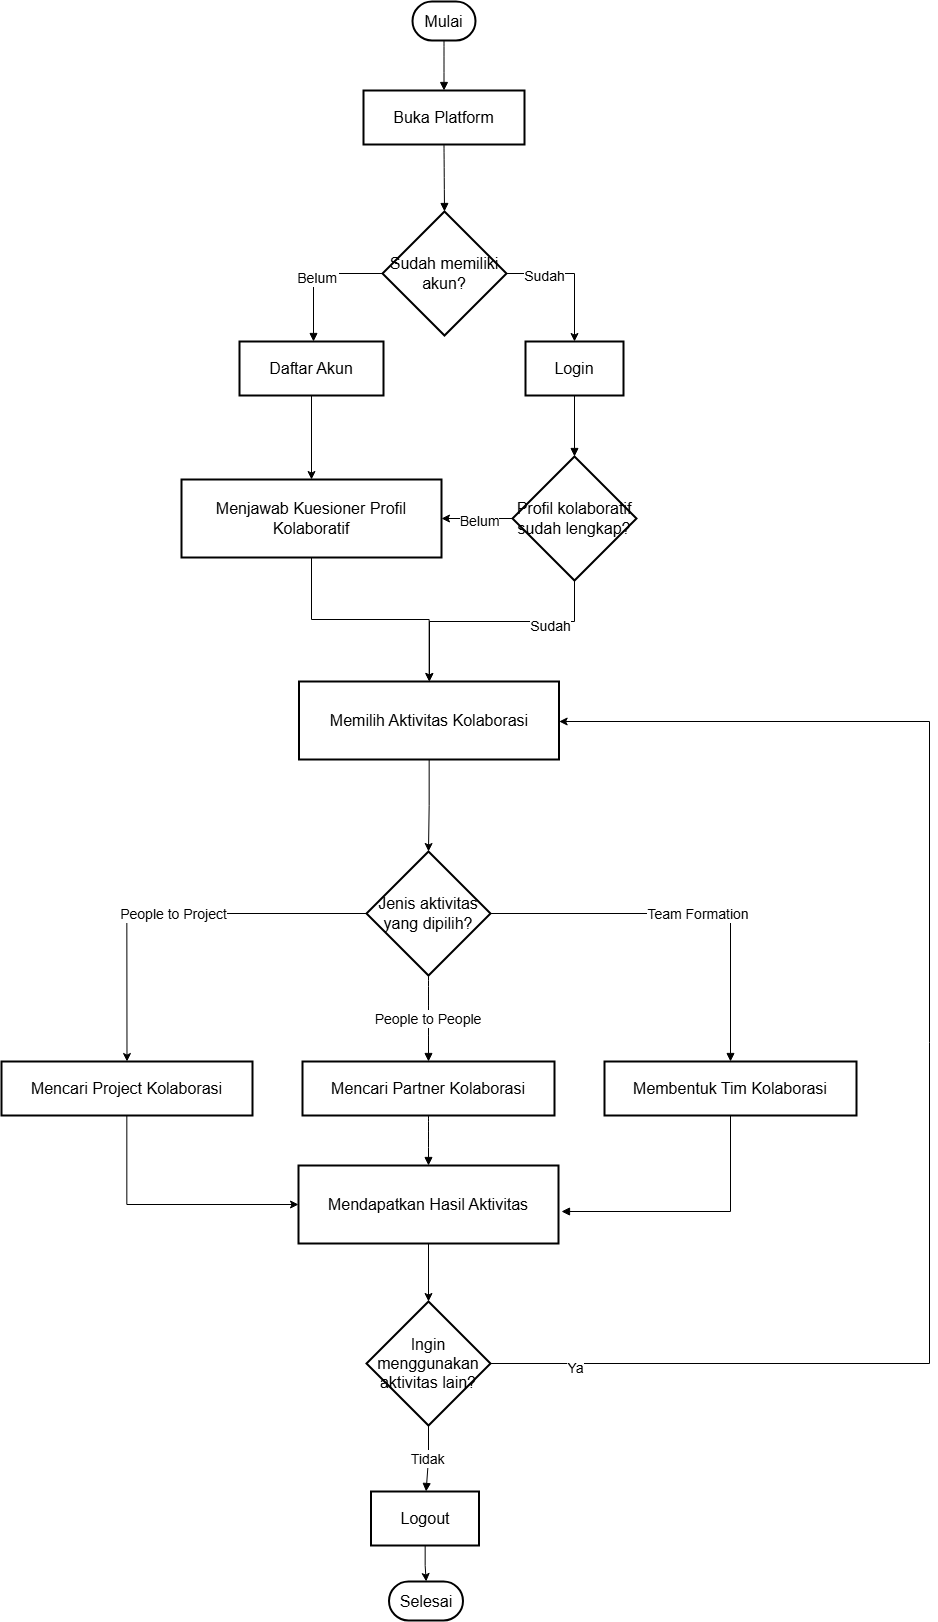
\includegraphics[width=0.75\textwidth]{images/flowchartsistem.png}
  \caption{\emph{Flowchart} Sistem}
  \label{fig:flowchart-sistem}
\end{figure}

\subsection{Batasan Sistem}

Dalam pengembangan perangkat lunak ini, terdapat beberapa batasan yang perlu diperhatikan guna memastikan fungsionalitas dan ketergantungannya terhadap sistem lain. Batasan tersebut antara lain:

\begin{enumerate}
  \item Sistem ditujukan khusus untuk mahasiswa sebagai pengguna utama.
  \item Sistem dikembangkan dalam bentuk aplikasi \emph{mobile} berbasis Android dan tidak mencakup platform lain seperti iOS maupun \emph{web browser}.
  \item Sistem hanya mencakup fungsionalitas yang berkaitan dengan pencarian rekan kolaborasi, pencarian kegiatan dan proyek eksternal, serta pembentukan tim. Fungsionalitas di luar ketiga hal tersebut, tidak termasuk dalam cakupan sistem.
  \item Proses rekomendasi dan pencocokan hanya menggunakan data profil yang diisikan secara mandiri oleh pengguna.
  \item Sistem tidak terintegrasi dengan sistem informasi akademik institusi manapun.
  \item Pengujian sistem dilakukan dalam lingkup terbatas dengan melibatkan responden mahasiswa sebagai sampel.
\end{enumerate}

\subsection{Dekomposisi Sistem}

Pada sistem aplikasi pencarian kolaborasi mahasiswa, dekomposisi dilakukan berdasarkan fungsi utama sistem, yaitu fungsi pencocokan atau \emph{matching}. Sistem ini tidak hanya memiliki satu bentuk pencocokan, melainkan terdiri dari beberapa kebutuhan pencocokan yang berbeda. Pertama, sistem perlu menyediakan fungsi untuk mencocokkan pengguna dengan pengguna lain. Kedua, sistem perlu menyediakan fungsi untuk mencocokkan pengguna dengan proyek atau peluang kolaborasi. Ketiga, sistem perlu menyediakan fungsi untuk membentuk tim dari beberapa pengguna berdasarkan kesesuaian peran, keterampilan, dan preferensi kerja sama.

Berdasarkan pendekatan tersebut, sistem didekomposisi menjadi tiga fungsi utama, yaitu fungsi pencocokan antarindividu, fungsi pencocokan individu dengan proyek, dan fungsi pembentukan tim. Pembagian ini dilakukan agar setiap fungsi memiliki fokus yang jelas, tidak saling bercampur, dan dapat dikembangkan secara lebih terarah.

\begin{longtable}{p{0.6cm} p{4cm} >{\raggedright\arraybackslash}p{\dimexpr\linewidth-4.6cm-6\tabcolsep\relax}}
  \caption{Dekomposisi Fungsi Utama Sistem}
  \label{tab:dekomposisi-fungsi} \\
  \toprule
    \textbf{No.} & \textbf{Fungsi Utama Sistem} & \textbf{Deskripsi} \\
  \midrule
  \endfirsthead
  \multicolumn{3}{l}{\small\textit{Tabel~\ref{tab:dekomposisi-fungsi} Dekomposisi Fungsi Utama Sistem (lanjutan)}} \\
  \toprule
    \textbf{No.} & \textbf{Fungsi Utama Sistem} & \textbf{Deskripsi} \\
  \midrule
  \endhead
  \bottomrule
  \multicolumn{3}{r}{\textit{Bersambung ke halaman berikutnya.}} \\
  \endfoot
  \bottomrule
  \endlastfoot
    1 & Pencocokan antarindividu & Fungsi ini digunakan untuk mencocokkan satu pengguna dengan pengguna lain berdasarkan profil, keterampilan, minat, pengalaman, dan preferensi kolaborasi. \\
    \midrule
    2 & Pencocokan individu dengan proyek & Fungsi ini digunakan untuk mencocokkan pengguna dengan proyek atau peluang kolaborasi berdasarkan kesesuaian antara profil pengguna dan kebutuhan proyek. \\
    \midrule
    3 & Pembentukan tim & Fungsi ini digunakan untuk membentuk komposisi tim dari beberapa pengguna berdasarkan kebutuhan peran, keterampilan, dan kecocokan antaranggota. \\
\end{longtable}

Setelah fungsi utama sistem berhasil diidentifikasi langkah berikutnya adalah melakukan dekomposisi lebih lanjut untuk menggambarkan rincian proses yang berada di dalam fungsi masing-masing. Dekomposisi ini bertujuan untuk menunjukkan bagaimana setiap fungsi utama diimplementasikan melalui serangkaian aktivitas yang saling berkaitan. Hasil dekomposisi fungsi tersebut ditunjukkan pada Gambar~\ref{fig:dekomposisi-sistem} berikut.

\begin{figure}[H]
  \centering
  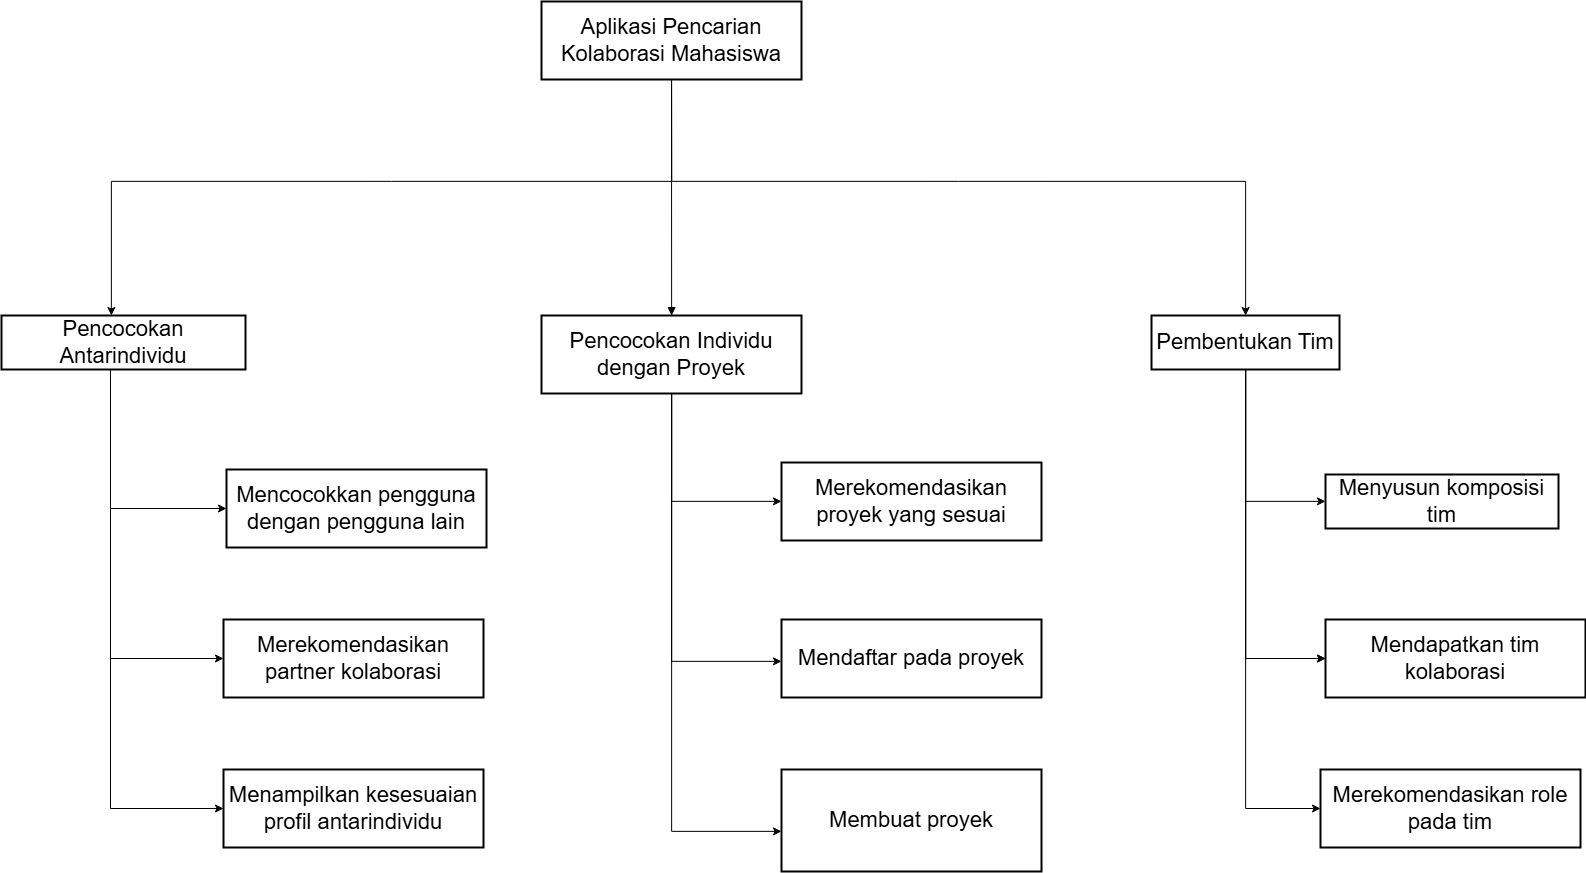
\includegraphics[width=\textwidth]{images/dekomposisisistem.png}
  \caption{Dekomposisi Sistem}
  \label{fig:dekomposisi-sistem}
\end{figure}

\subsection{Pembagian Modul}

Berdasarkan hasil dekomposisi sistem, setiap fungsi utama yang telah diidentifikasi kemudian direpresentasikan ke dalam modul sistem. Pembagian modul ini dilakukan agar setiap fungsi memiliki ruang lingkup pengembangan yang jelas dan tidak bercampur dengan fungsi lainnya. Dengan demikian, setiap modul memiliki tanggung jawab utama yang spesifik sesuai dengan fungsi yang diwakilinya.

Dalam sistem aplikasi pencarian kolaborasi mahasiswa, terdapat tiga fungsi utama yang kemudian dikembangkan menjadi tiga modul. Fungsi pencocokan antarindividu direpresentasikan melalui modul \emph{People-to-People}, fungsi pencocokan individu dengan proyek direpresentasikan melalui modul \emph{People-to-Project}, sedangkan fungsi pembentukan tim direpresentasikan melalui modul \emph{Team Formation}. Setiap detail dari modul dapat dilihat pada Tabel~\ref{tab:pembagian-modul} berikut.

\begin{longtable}{p{2.5cm} p{3.5cm} p{3.5cm} p{\dimexpr\linewidth-9.5cm-8\tabcolsep\relax}}
  \caption{Pembagian Modul Sistem}
  \label{tab:pembagian-modul} \\
  \toprule
  \textbf{Aspek} & \textbf{\emph{People-to-People}} & \textbf{\emph{People-to-Project}} & \textbf{\emph{Team Formation}} \\
  \midrule
  \endfirsthead
  \multicolumn{4}{l}{\small\textit{Tabel~\ref{tab:pembagian-modul} Pembagian Modul Sistem (lanjutan)}} \\
  \toprule
  \textbf{Aspek} & \textbf{\emph{People-to-People}} & \textbf{\emph{People-to-Project}} & \textbf{\emph{Team Formation}} \\
  \midrule
  \endhead
  \bottomrule
  \multicolumn{4}{r}{\textit{Bersambung ke halaman berikutnya.}} \\
  \endfoot
  \bottomrule
  \endlastfoot
  Fungsi utama & Mencocokkan pengguna dengan pengguna lain & Mencocokkan pengguna dengan proyek atau lowongan kolaborasi & Membentuk tim dari beberapa pengguna \\
  \midrule
  Objek pencocokan & Orang dengan orang & Orang dengan proyek & Beberapa orang dalam satu tim \\
  \midrule
  Pola relasi & \emph{Individual-to-individual matching} & \emph{Individual-to-opportunity/project matching} & \emph{Group/team-based matching} \\
  \midrule
  Contoh kebutuhan pengguna & ``Saya ingin mencari mitra yang cocok untuk belajar, riset, lomba, atau \emph{project}.'' & ``Saya ingin mencari proyek yang sesuai dengan \emph{skill} dan minat saya.'' & ``Saya ingin membentuk atau bergabung ke tim yang lengkap dan seimbang untuk mengikuti lomba atau mengerjakan \emph{project}.'' \\
  \midrule
  Aktor utama & Mahasiswa sebagai pencari mitra & Mahasiswa dan pemilik/pengelola proyek & Mahasiswa yang ingin membentuk atau bergabung dengan tim \\
  \midrule
  Input utama & Data Mahasiswa & Data Mahasiswa dan proyek & Data anggota tim \\
  \midrule
  Proses utama & Menghitung kecocokan antara satu pengguna dengan pengguna lain & Menghitung kesesuaian antara profil pengguna dan kebutuhan proyek & Menyusun kombinasi anggota berdasarkan \emph{role}, \emph{skill}, dan kecocokan tim \\
  \midrule
  Output utama & Rekomendasi mitra atau pengguna yang cocok & Rekomendasi proyek untuk pengguna atau kandidat untuk proyek & Rekomendasi komposisi tim dan anggota yang sesuai \\
  \midrule
  Hasil akhir & Pengguna menemukan mitra potensial & Pengguna menemukan proyek atau proyek menemukan kandidat & Pengguna mendapatkan tim dengan \emph{role} yang sesuai dan tim yang efektif \\
\end{longtable}

Setiap modul yang terdapat dalam sistem dikerjakan secara kolaboratif dengan pembagian tanggung jawab yang disesuaikan berdasarkan ruang lingkup dan kompleksitas pekerjaan anggota tim masing-masing. Pembagian ini bertujuan untuk memastikan seluruh kebutuhan pengembangan sistem dapat diselesaikan secara efektif, terstruktur, dan sesuai dengan kompetensi yang dimiliki oleh setiap anggota. Rincian pembagian pengerjaan modul untuk anggota masing-masing dapat dilihat pada Tabel~\ref{tab:pic-modul} berikut.

\begin{longtable}{p{0.6cm} p{4cm} >{\raggedright\arraybackslash}p{\dimexpr\linewidth-4.6cm-6\tabcolsep\relax}}
  \caption{Pembagian Pengerjaan Modul}
  \label{tab:pic-modul} \\
  \toprule
    \textbf{No} & \textbf{Modul} & \textbf{PIC} \\
  \midrule
  \endfirsthead
  \multicolumn{3}{l}{\small\textit{Tabel~\ref{tab:pic-modul} Pembagian Pengerjaan Modul (lanjutan)}} \\
  \toprule
    \textbf{No} & \textbf{Modul} & \textbf{PIC} \\
  \midrule
  \endhead
  \bottomrule
  \multicolumn{3}{r}{\textit{Bersambung ke halaman berikutnya.}} \\
  \endfoot
  \bottomrule
  \endlastfoot
    1 & \emph{People-to-People} & Ahmad Fawwazi (182221) \\
    \midrule
    2 & \emph{People-to-Project} & Muhammad Faishal Putra (182221) \\
    \midrule
    3 & \emph{Team Formation} & Muhammad Faishal Firdaus (18222136) \\
\end{longtable}

\subsection{Modul \emph{People-to-Project}}

Modul \emph{People-to-Project} merupakan bagian dari sistem yang berfokus pada proses pencarian dan pencocokan antara mahasiswa dengan kegiatan kolaboratif atau proyek yang tersedia di platform. Modul ini dirancang untuk membantu mahasiswa menemukan kegiatan kolaboratif yang sesuai dengan minat dan kemampuannya, melihat detail kegiatan beserta kebutuhan \emph{role}, mendaftarkan diri pada \emph{role} yang diminati, atau membuat dan mempublikasikan kegiatan kolaboratif baru bagi mahasiswa lain untuk bergabung. Berbeda dari modul \emph{People-to-People} yang berorientasi pada pencarian individu ke individu, modul ini menempatkan kegiatan kolaboratif (\emph{project}) sebagai objek utama yang ditemukan melalui mekanisme \emph{feed} rekomendasi, yaitu tampilan yang menyajikan daftar kegiatan aktif terurut berdasarkan skor kecocokan hasil \emph{affinity based matching} antara profil mahasiswa dan kebutuhan kegiatan.

Dalam modul ini, pengguna dapat melihat informasi kegiatan, seperti deskripsi, kategori, \emph{timeline}, kebutuhan \emph{role} beserta \emph{skill} yang dicari, dan sisa kuota setiap \emph{role}. Sistem juga mendukung rekomendasi kegiatan berdasarkan profil dan preferensi kolaborasi mahasiswa, serta menampilkan skor kecocokan dan rincian komponen penilaiannya (\emph{affinity score breakdown}) untuk setiap kegiatan yang direkomendasikan. Selama kuota \emph{role} kegiatan belum terpenuhi, mahasiswa dapat mengajukan pendaftaran pada \emph{role} yang diminati, sementara mahasiswa yang berperan sebagai pembuat kegiatan dapat meninjau daftar pendaftar dan menentukan keputusan terima atau tolak untuk setiap pengajuan berdasarkan kesesuaian \emph{role}. Dengan demikian, modul \emph{People-to-Project} tidak hanya menyediakan fitur pencarian kegiatan, tetapi juga mendukung proses pendaftaran dan seleksi anggota yang lebih terarah dan berbasis kecocokan.

\subsection{Aktor Pada Modul}

Setiap aktor memiliki peran, tanggung jawab, serta hak akses yang berbeda sesuai dengan fungsi yang dijalankan dalam sistem. Pendefinisian tugas dan hak akses ini bertujuan untuk memastikan bahwa setiap aktor hanya dapat mengakses dan melakukan aktivitas yang sesuai dengan kewenangannya. Deskripsi tugas dan hak akses aktor pada modul \emph{People-to-People Recommendation} terdapat pada Tabel~\ref{tab:aktor-modul} berikut.

\begin{longtable}{p{2cm} p{5.5cm} >{\raggedright\arraybackslash}p{\dimexpr\linewidth-7.5cm-6\tabcolsep\relax}}
  \caption{Aktor Pada Modul}
  \label{tab:aktor-modul} \\
  \toprule
    \textbf{Kategori Pengguna} & \textbf{Tugas} & \textbf{Hak Akses ke Aplikasi} \\
  \midrule
  \endfirsthead
  \multicolumn{3}{l}{\small\textit{Tabel~\ref{tab:aktor-modul} Aktor Pada Modul (lanjutan)}} \\
  \toprule
    \textbf{Kategori Pengguna} & \textbf{Tugas} & \textbf{Hak Akses ke Aplikasi} \\
  \midrule
  \endhead
  \bottomrule
  \multicolumn{3}{r}{\textit{Bersambung ke halaman berikutnya.}} \\
  \endfoot
  \bottomrule
  \endlastfoot
    Mahasiswa & Pengguna utama modul yang memanfaatkan fitur rekomendasi mitra kolaborasi. Mahasiswa mengisi dan memperbarui profil kolaboratif, melihat \emph{feed} rekomendasi, melihat detail profil calon mitra, serta melakukan interaksi dasar terhadap hasil rekomendasi. & Mengelola profil dan preferensi kolaborasi; melihat \emph{feed} rekomendasi calon mitra; melihat detail profil calon mitra; melakukan interaksi berupa \emph{save profile}, \emph{express interest}, dan \emph{connect request}; mengatur visibilitas profil; dan melakukan filter pada \emph{feed} rekomendasi. \\
\end{longtable}

\subsection{Batasan Modul}

Dalam pengembangan modul \emph{People-to-Project Recommendation}, terdapat beberapa batasan yang perlu diperhatikan guna memastikan fokus dan kelayakan implementasi modul. Batasan tersebut adalah sebagai berikut.

\begin{enumerate}
  \item Modul difokuskan pada rekomendasi antarindividu dengan kegiatan kolaboratif yang sesuai.
  \item Penilaian kecocokan antarmahasiswa hanya menggunakan data profil yang diisikan secara mandiri oleh pengguna melalui kuesioner \emph{onboarding} dan form pengisian profil, mencakup minat, keterampilan, pengalaman, preferensi gaya kerja, dan ketersediaan waktu.
  \item Modul tidak mencakup fase interaksi lanjutan setelah koneksi terbentuk, seperti manajemen kolaborasi, komunikasi berkelanjutan, atau penjadwalan bersama.
  \item Mekanisme \emph{Affinity Based Matching} dirancang berdasarkan pembobotan atribut dari literatur ilmiah tanpa melakukan pembuktian matematis formal atau validasi komputasional tingkat lanjut.
  \item Modul tidak terintegrasi dengan sistem informasi akademik institusi manapun.
  \item Pengujian modul dilakukan dalam lingkup terbatas dan tidak dirancang untuk \emph{deployment} dalam skala produksi.
\end{enumerate}

\subsection{\emph{Flowchart} Modul}

Modul \emph{People-to-Project Recommendation} menggambarkan alur interaksi pengguna dengan sistem dalam proses pencarian dan rekomendasi kegiatan kolaboratif. \emph{Flowchart} modul \emph{People-to-Project} digambarkan pada Gambar~\ref{fig:flowchart-modul} berikut.

\begin{figure}[H]
  \centering
  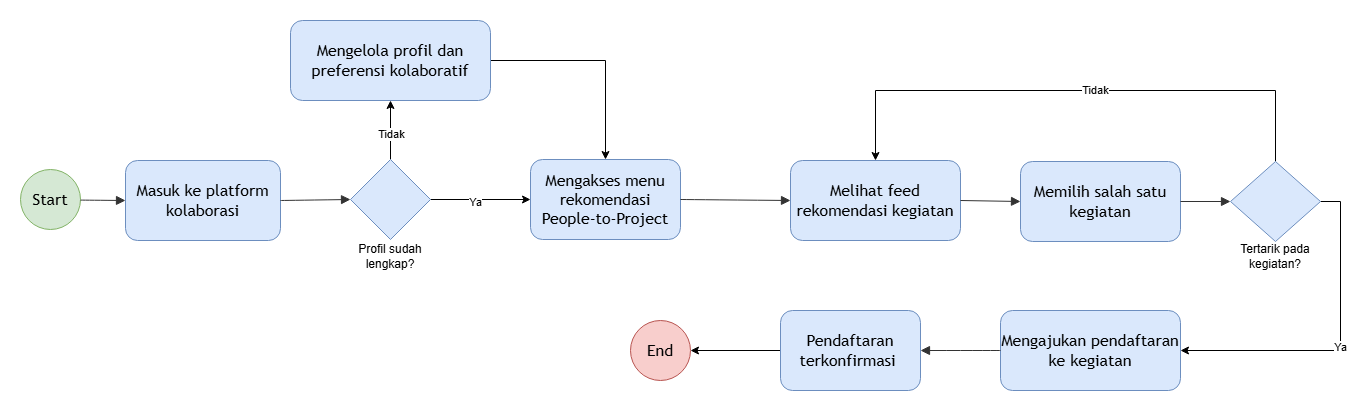
\includegraphics[width=\textwidth]{images/flowchartmodul.png}
  \caption{\emph{Flowchart} Modul \emph{People-to-Project}}
  \label{fig:flowchart-modul}
\end{figure}

Alur dimulai ketika pengguna mengakses modul \emph{People-to-Project}. Sistem kemudian memeriksa kelengkapan profil pengguna. Apabila profil belum lengkap, pengguna diarahkan untuk mengisi atau memperbarui profil dan preferensi kolaboratifnya terlebih dahulu sebelum dapat melanjutkan. Proses ini berulang hingga profil dinyatakan lengkap oleh sistem. Setelah profil lengkap, sistem menampilkan \emph{feed} rekomendasi kegiatan kolaboratif yang telah diurutkan berdasarkan skor kecocokan hasil perhitungan \emph{Affinity Based Matching} antara profil mahasiswa dan kebutuhan kegiatan. Pengguna kemudian memilih salah satu kegiatan dari daftar tersebut untuk dilihat detailnya lebih lanjut. Apabila pengguna menilai kegiatan tersebut tidak cocok atau tidak tertarik, pengguna dapat kembali ke \emph{feed} rekomendasi dan memilih kegiatan lain. Apabila pengguna menilai kegiatan tersebut cocok dan tertarik untuk bergabung, pengguna dapat mengajukan pendaftaran pada \emph{role} yang diminati di kegiatan tersebut. Setelah pengajuan pendaftaran diproses dan dikonfirmasi oleh pembuat kegiatan, mahasiswa resmi tergabung dalam kegiatan tersebut dan alur modul selesai.

% ==========================================
\section{Perancangan Model Sistem}

\subsection{\emph{Use Case} Diagram}

\emph{Use case} diagram terdapat pada Gambar~\ref{fig:use-case-diagram} berikut.

\begin{figure}[H]
  \centering
  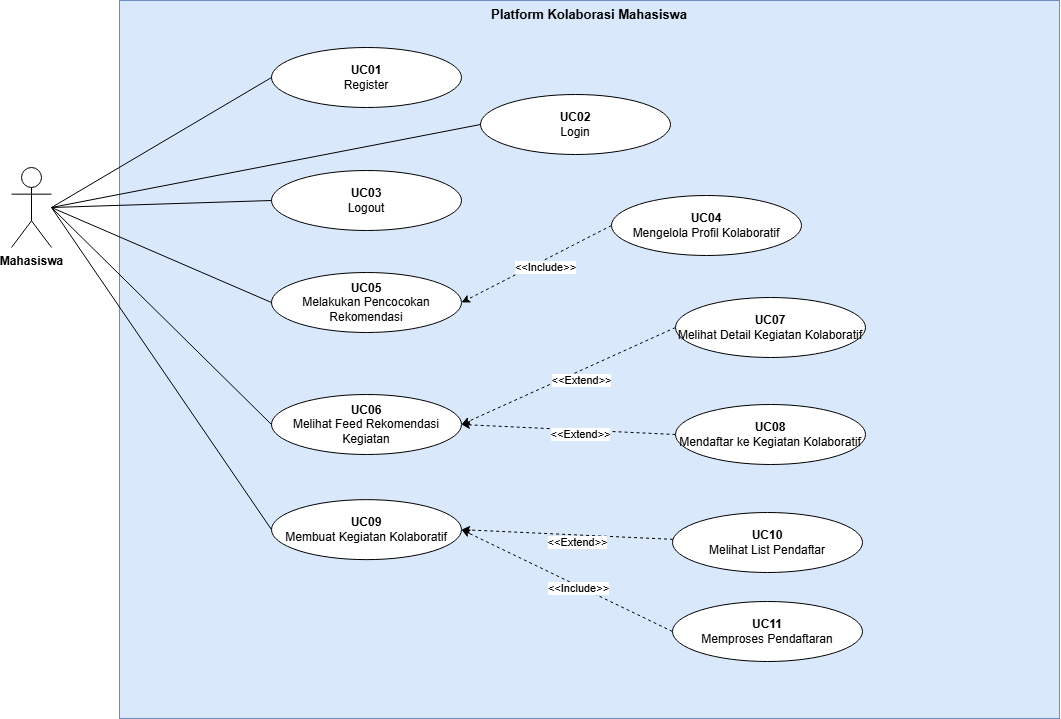
\includegraphics[width=\textwidth]{images/UseCaseDiagram.png}
  \caption{\emph{Use Case} Diagram Platform Kolaborasi Mahasiswa}
  \label{fig:use-case-diagram}
\end{figure}

Gambar~\ref{fig:use-case-diagram} menunjukkan \emph{Use Case} Diagram Platform Kolaborasi Mahasiswa yang menggambarkan interaksi aktor Mahasiswa dengan sistem, mulai dari registrasi, \emph{login}, dan \emph{logout}, hingga mengelola profil kolaboratif, memperoleh rekomendasi kegiatan, melihat \emph{feed} dan detail kegiatan, mendaftar ke kegiatan kolaboratif, serta membuat dan mengelola kegiatan yang dibuat. Diagram juga memperlihatkan hubungan \emph{include} dan \emph{extend} antar-\emph{use case} untuk menunjukkan keterkaitan proses dalam sistem. Penjelasan lebih rinci mengenai setiap \emph{use case} dapat dilihat pada Tabel~\ref{tab:uc-list} berikut.

\begin{longtable}{p{1.5cm} p{4.5cm} p{2cm} p{\dimexpr\linewidth-8cm-8\tabcolsep\relax}}
  \caption{Daftar \emph{Use Case}}
  \label{tab:uc-list} \\
  \toprule
  \textbf{Kode \emph{Use Case}} & \textbf{Nama \emph{Use Case}} & \textbf{Aktor Utama} & \textbf{Penjelasan Detail \emph{Use Case}} \\
  \midrule
  \endfirsthead
  \multicolumn{4}{l}{\small\textit{Tabel~\ref{tab:uc-list} Daftar \emph{Use Case} (lanjutan)}} \\
  \toprule
  \textbf{Kode \emph{Use Case}} & \textbf{Nama \emph{Use Case}} & \textbf{Aktor Utama} & \textbf{Penjelasan Detail \emph{Use Case}} \\
  \midrule
  \endhead
  \bottomrule
  \multicolumn{4}{r}{\textit{Bersambung ke halaman berikutnya.}} \\
  \endfoot
  \bottomrule
  \endlastfoot
  UC01 & Register & Mahasiswa & Mahasiswa membuat akun baru pada platform dengan mengisi data diri meliputi nama lengkap, \emph{email}, institusi, dan kata sandi. Akun yang berhasil dibuat menjadi syarat untuk dapat mengakses seluruh fitur platform. \\
  \midrule
  UC02 & \emph{Login} & Mahasiswa & Mahasiswa mengautentikasi diri ke dalam platform menggunakan \emph{email} dan kata sandi yang telah didaftarkan. Setelah berhasil, sistem membuat sesi aktif dan mahasiswa dapat mengakses seluruh fitur. \\
  \midrule
  UC03 & \emph{Logout} & Mahasiswa & Mahasiswa mengakhiri sesi aktifnya pada platform. Sistem menghapus data sesi dan mengarahkan mahasiswa kembali ke halaman \emph{login}. \\
  \midrule
  UC04 & Mengelola Profil Kolaboratif & Mahasiswa & Mahasiswa mengisi atau memperbarui data profil kolaboratifnya melalui kuesioner yang mencakup minat, \emph{skill}, pengalaman, preferensi peran, dan ketersediaan waktu. Data ini menjadi dasar utama dalam proses pencocokan rekomendasi kegiatan. \\
  \midrule
  UC05 & Melakukan Pencocokan Rekomendasi & Mahasiswa & Sistem menjalankan mekanisme \emph{affinity based matching} secara otomatis ketika mahasiswa mengakses \emph{feed} rekomendasi. Sistem membaca profil mahasiswa, membandingkannya dengan kebutuhan setiap kegiatan aktif, menghitung skor kecocokan, dan menyimpan hasilnya. \\
  \midrule
  UC06 & Melihat \emph{Feed} Rekomendasi Kegiatan & Mahasiswa & Mahasiswa melihat daftar kegiatan kolaboratif yang telah diurutkan berdasarkan skor kecocokan tertinggi. Setiap item pada \emph{feed} menampilkan ringkasan kegiatan dan indikator skor kecocokan. \\
  \midrule
  UC07 & Melihat Detail Kegiatan Kolaboratif & Mahasiswa & Mahasiswa mengakses halaman detail suatu kegiatan yang menampilkan informasi lengkap meliputi deskripsi, kategori, \emph{role} yang dibutuhkan, \emph{skill} yang dicari per \emph{role}, kuota, \emph{timeline}, dan skor kecocokan mahasiswa terhadap kegiatan tersebut beserta penjelasan faktor yang berkontribusi. \\
  \midrule
  UC08 & Mendaftar ke Kegiatan Kolaboratif & Mahasiswa & Mahasiswa mengajukan pendaftaran diri ke kegiatan yang dipilih dengan memilih \emph{role} yang ingin dilamar. Sistem mencatat pendaftaran dengan status ``Menunggu'' dan mengirimkan notifikasi kepada pembuat kegiatan. \\
  \midrule
  UC09 & Membuat Kegiatan Kolaboratif & Mahasiswa & Mahasiswa yang memiliki inisiatif dapat membuat dan mempublikasikan kegiatan kolaboratif baru. Dalam proses ini mahasiswa mendefinisikan judul, deskripsi, kategori, \emph{role} yang dibutuhkan beserta \emph{skill} dan kuota per \emph{role}, serta \emph{timeline} kegiatan. \\
  \midrule
  UC10 & Melihat List Pendaftar & Mahasiswa & Mahasiswa yang berperan sebagai pembuat kegiatan dapat melihat daftar seluruh mahasiswa yang telah mengajukan pendaftaran ke kegiatannya, disertai informasi \emph{role} yang dilamar, skor kecocokan pendaftar, dan status pendaftaran saat ini. \\
  \midrule
  UC11 & Memproses Pendaftaran & Mahasiswa & Pembuat kegiatan dapat menerima atau menolak setiap pendaftar yang masuk. Keputusan yang diambil akan mengubah status pendaftaran dan memicu notifikasi kepada mahasiswa pendaftar yang bersangkutan. \\
\end{longtable}

Pemetaan kebutuhan fungsional dengan \emph{use case} sistem terdapat pada Tabel~\ref{tab:uc-traceability} berikut.

\begin{longtable}{p{3cm} p{6cm} >{\raggedright\arraybackslash}p{\dimexpr\linewidth-9cm-6\tabcolsep\relax}}
  \caption{\emph{Traceability Use Case}}
  \label{tab:uc-traceability} \\
  \toprule
    \textbf{Kode \emph{Use Case}} & \textbf{Nama \emph{Use Case}} & \textbf{Kode FR Terkait} \\
  \midrule
  \endfirsthead
  \multicolumn{3}{l}{\small\textit{Tabel~\ref{tab:uc-traceability} \emph{Traceability Use Case} (lanjutan)}} \\
  \toprule
    \textbf{Kode \emph{Use Case}} & \textbf{Nama \emph{Use Case}} & \textbf{Kode FR Terkait} \\
  \midrule
  \endhead
  \bottomrule
  \multicolumn{3}{r}{\textit{Bersambung ke halaman berikutnya.}} \\
  \endfoot
  \bottomrule
  \endlastfoot
    UC01 & Register & -- \\
    \midrule
    UC02 & \emph{Login} & -- \\
    \midrule
    UC03 & \emph{Logout} & -- \\
    \midrule
    UC04 & Mengelola Profil Kolaboratif & FR01 \\
    \midrule
    UC05 & Melakukan Pencocokan Rekomendasi & FR02 \\
    \midrule
    UC06 & Melihat \emph{Feed} Rekomendasi Kegiatan & FR03 \\
    \midrule
    UC07 & Melihat Detail Kegiatan Kolaboratif & FR04 \\
    \midrule
    UC08 & Mendaftar ke Kegiatan Kolaboratif & FR05 \\
    \midrule
    UC09 & Membuat Kegiatan Kolaboratif & FR06 \\
    \midrule
    UC10 & Melihat List Pendaftar & FR07 \\
    \midrule
    UC11 & Memproses Pendaftaran & FR08 \\
\end{longtable}

% ==========================================
\subsection{Deskripsi \emph{Use Case}}

Deskripsi \emph{use case} memberikan penjelasan mengenai tujuan penggunaan fitur, aktor yang terlibat, kondisi yang harus dipenuhi sebelum proses dijalankan, alur interaksi antara pengguna dan sistem, serta kondisi akhir yang dihasilkan setelah proses selesai. Pendefinisian ini bertujuan untuk memastikan setiap kebutuhan fungsional terdokumentasi secara jelas dan dapat menjadi acuan dalam proses perancangan, implementasi, maupun pengujian sistem. Deskripsi \emph{use case} masing-masing disajikan pada tabel-tabel berikut.

\subsubsection{Deskripsi UC01}

Deskripsi \emph{use case} untuk UC01 Register terdapat pada Tabel~\ref{tab:uc01} berikut.

\begin{longtable}{>{\raggedright\arraybackslash}p{5cm} >{\raggedright\arraybackslash}p{\dimexpr\linewidth-5cm-4\tabcolsep\relax}}
  \caption{Deskripsi \emph{Use Case} UC01 -- Register}
  \label{tab:uc01} \\
  \toprule
  \textbf{Komponen} & \textbf{Keterangan} \\
  \midrule
  \endfirsthead
  \multicolumn{2}{l}{\small\textit{Tabel~\ref{tab:uc01} Deskripsi \emph{Use Case} UC01 -- Register (lanjutan)}} \\
  \toprule
  \textbf{Komponen} & \textbf{Keterangan} \\
  \midrule
  \endhead
  \bottomrule
  \multicolumn{2}{r}{\textit{Bersambung ke halaman berikutnya.}} \\
  \endfoot
  \bottomrule
  \endlastfoot
  \textbf{Kode/Nama \emph{Use Case}} & UC01 / Register \\
  \midrule
  \textbf{Tujuan} & Memungkinkan mahasiswa membuat akun baru pada platform untuk mengakses seluruh fitur aplikasi. \\
  \midrule
  \textbf{\emph{Main Actor}} & Mahasiswa \\
  \midrule
  \textbf{\emph{Prerequisite Use Case}} & -- \\
  \midrule
  \textbf{\emph{Entry Condition}} & Pengguna belum memiliki akun pada platform. Pengguna berada pada halaman awal aplikasi. \\
  \midrule
  \textbf{Data} & Nama lengkap, \emph{email}, \emph{password}, konfirmasi \emph{password}. \\
  \midrule
  \textbf{\emph{Stimulus}} & Pengguna memilih opsi Register pada halaman awal aplikasi. \\
  \midrule
  \textbf{\emph{Response}} & Sistem memvalidasi data yang dimasukkan dan membuat akun baru apabila data valid. \\
  \midrule
  \textbf{\emph{Postcondition}} & Akun baru berhasil dibuat dan pengguna diarahkan ke halaman \emph{Login}. \\
\end{longtable}

Skenario \emph{use case} UC01 Register terdapat pada Tabel~\ref{tab:uc01-skenario} berikut.

\begin{longtable}{>{\raggedright\arraybackslash}p{5cm} >{\raggedright\arraybackslash}p{\dimexpr\linewidth-5cm-4\tabcolsep\relax}}
  \caption{Skenario \emph{Use Case} UC01 -- Register}
  \label{tab:uc01-skenario} \\
  \toprule
  \textbf{Aksi Pengguna} & \textbf{Reaksi Sistem} \\
  \midrule
  \endfirsthead
  \multicolumn{2}{l}{\small\textit{Tabel~\ref{tab:uc01-skenario} Skenario \emph{Use Case} UC01 -- Register (lanjutan)}} \\
  \toprule
  \textbf{Aksi Pengguna} & \textbf{Reaksi Sistem} \\
  \midrule
  \endhead
  \bottomrule
  \multicolumn{2}{r}{\textit{Bersambung ke halaman berikutnya.}} \\
  \endfoot
  \bottomrule
  \endlastfoot
  \multicolumn{2}{l}{\textbf{Skenario Normal: Pengguna berhasil membuat akun baru}} \\
  \midrule
  Pengguna memilih opsi Register pada halaman awal. & \\
  \midrule
  Pengguna mengisi nama lengkap, \emph{email}, \emph{password}, dan konfirmasi \emph{password}. & \\
  \midrule
  Pengguna menekan tombol Register. & \\
  \midrule
   & Sistem memvalidasi seluruh data yang dimasukkan. \\
  \midrule
   & Sistem membuat akun baru dan menyimpan data ke basis data. \\
  \midrule
   & Sistem menampilkan pesan registrasi berhasil dan mengarahkan pengguna ke halaman \emph{Login}. \\
  \midrule
  Pengguna melihat pesan registrasi berhasil dan diarahkan ke halaman \emph{login}. & \\
  \midrule
  \multicolumn{2}{l}{\textbf{Skenario Alternatif: \emph{Email} sudah terdaftar}} \\
  \midrule
  Pengguna mengisi data registrasi dengan \emph{email} yang sudah terdaftar. & \\
  \midrule
  Pengguna menekan tombol Register. & \\
  \midrule
   & Sistem mendeteksi bahwa \emph{email} sudah terdaftar. \\
  \midrule
   & Sistem menampilkan pesan bahwa \emph{email} sudah digunakan dan meminta pengguna menggunakan \emph{email} lain. \\
  \midrule
  Pengguna melihat pesan bahwa \emph{email} sudah digunakan dan diminta untuk menggunakan \emph{email} lain. & \\
  \midrule
  \multicolumn{2}{l}{\textbf{Skenario Alternatif: Input Tidak Valid}} \\
  \midrule
  Pengguna memilih opsi Register pada halaman awal. & \\
  \midrule
  Pengguna mengisi nama lengkap, \emph{email}, \emph{password}, dan konfirmasi \emph{password}. & \\
  \midrule
  Pengguna menekan tombol Register. & \\
  \midrule
   & Sistem memvalidasi seluruh data yang dimasukkan. \\
  \midrule
   & Sistem mendeteksi bahwa input tidak valid. \\
  \midrule
   & Sistem menampilkan pesan bahwa input tidak valid dengan keterangan detail. \\
  \midrule
  Pengguna melihat pesan bahwa input tidak valid dengan keterangan detail. & \\
\end{longtable}

\subsubsection{Deskripsi UC02}

Deskripsi \emph{use case} untuk UC02 \emph{Login} terdapat pada Tabel~\ref{tab:uc02} berikut.

\begin{longtable}{>{\raggedright\arraybackslash}p{5cm} >{\raggedright\arraybackslash}p{\dimexpr\linewidth-5cm-4\tabcolsep\relax}}
  \caption{Deskripsi \emph{Use Case} UC02 -- \emph{Login}}
  \label{tab:uc02} \\
  \toprule
  \textbf{Komponen} & \textbf{Keterangan} \\
  \midrule
  \endfirsthead
  \multicolumn{2}{l}{\small\textit{Tabel~\ref{tab:uc02} Deskripsi \emph{Use Case} UC02 -- \emph{Login} (lanjutan)}} \\
  \toprule
  \textbf{Komponen} & \textbf{Keterangan} \\
  \midrule
  \endhead
  \bottomrule
  \multicolumn{2}{r}{\textit{Bersambung ke halaman berikutnya.}} \\
  \endfoot
  \bottomrule
  \endlastfoot
  \textbf{Kode/Nama \emph{Use Case}} & UC02 / \emph{Login} \\
  \midrule
  \textbf{Tujuan} & Memungkinkan mahasiswa masuk ke dalam platform menggunakan kredensial yang telah didaftarkan. \\
  \midrule
  \textbf{\emph{Main Actor}} & Mahasiswa \\
  \midrule
  \textbf{\emph{Prerequisite Use Case}} & UC01 / Register \\
  \midrule
  \textbf{\emph{Entry Condition}} & Pengguna sudah memiliki akun pada platform. Pengguna berada pada halaman \emph{Login}. \\
  \midrule
  \textbf{Data} & \emph{Email}, \emph{password}. \\
  \midrule
  \textbf{\emph{Stimulus}} & Pengguna memilih opsi \emph{Login} pada halaman awal aplikasi. \\
  \midrule
  \textbf{\emph{Response}} & Sistem memvalidasi kredensial yang dimasukkan dan memberikan akses ke platform apabila kredensial valid. \\
  \midrule
  \textbf{\emph{Postcondition}} & Pengguna berhasil masuk dan diarahkan ke halaman utama platform. \\
\end{longtable}

Skenario \emph{use case} UC02 \emph{Login} terdapat pada Tabel~\ref{tab:uc02-skenario} berikut.

\begin{longtable}{>{\raggedright\arraybackslash}p{5cm} >{\raggedright\arraybackslash}p{\dimexpr\linewidth-5cm-4\tabcolsep\relax}}
  \caption{Skenario \emph{Use Case} UC02 -- \emph{Login}}
  \label{tab:uc02-skenario} \\
  \toprule
  \textbf{Aksi Pengguna} & \textbf{Reaksi Sistem} \\
  \midrule
  \endfirsthead
  \multicolumn{2}{l}{\small\textit{Tabel~\ref{tab:uc02-skenario} Skenario \emph{Use Case} UC02 -- \emph{Login} (lanjutan)}} \\
  \toprule
  \textbf{Aksi Pengguna} & \textbf{Reaksi Sistem} \\
  \midrule
  \endhead
  \bottomrule
  \multicolumn{2}{r}{\textit{Bersambung ke halaman berikutnya.}} \\
  \endfoot
  \bottomrule
  \endlastfoot
  \multicolumn{2}{l}{\textbf{Skenario Normal: Pengguna berhasil masuk ke platform}} \\
  \midrule
  Pengguna memilih opsi \emph{Login} pada halaman awal. & \\
  \midrule
  Pengguna mengisi \emph{email} dan \emph{password}. & \\
  \midrule
  Pengguna menekan tombol \emph{Login}. & \\
  \midrule
   & Sistem memvalidasi kredensial yang dimasukkan. \\
  \midrule
   & Sistem membuat sesi aktif untuk pengguna. \\
  \midrule
   & Sistem mengarahkan pengguna ke halaman utama platform. \\
  \midrule
  Pengguna melihat halaman utama dengan akun pengguna. & \\
  \midrule
  \multicolumn{2}{l}{\textbf{Skenario Alternatif: Kredensial tidak valid}} \\
  \midrule
  Pengguna mengisi \emph{email} atau \emph{password} yang salah. & \\
  \midrule
  Pengguna menekan tombol \emph{Login}. & \\
  \midrule
   & Sistem mendeteksi bahwa kredensial tidak valid. \\
  \midrule
   & Sistem menampilkan pesan bahwa \emph{email} atau \emph{password} salah dan meminta pengguna mencoba kembali. \\
  \midrule
  Pengguna melihat pesan bahwa \emph{email} atau \emph{password} salah dan meminta pengguna mencoba kembali. & \\
\end{longtable}

\subsubsection{Deskripsi UC03}

Deskripsi \emph{use case} untuk UC03 \emph{Logout} terdapat pada Tabel~\ref{tab:uc03} berikut.

\begin{longtable}{>{\raggedright\arraybackslash}p{5cm} >{\raggedright\arraybackslash}p{\dimexpr\linewidth-5cm-4\tabcolsep\relax}}
  \caption{Deskripsi \emph{Use Case} UC03 -- \emph{Logout}}
  \label{tab:uc03} \\
  \toprule
  \textbf{Komponen} & \textbf{Keterangan} \\
  \midrule
  \endfirsthead
  \multicolumn{2}{l}{\small\textit{Tabel~\ref{tab:uc03} Deskripsi \emph{Use Case} UC03 -- \emph{Logout} (lanjutan)}} \\
  \toprule
  \textbf{Komponen} & \textbf{Keterangan} \\
  \midrule
  \endhead
  \bottomrule
  \multicolumn{2}{r}{\textit{Bersambung ke halaman berikutnya.}} \\
  \endfoot
  \bottomrule
  \endlastfoot
  \textbf{Kode/Nama \emph{Use Case}} & UC03 / \emph{Logout} \\
  \midrule
  \textbf{Tujuan} & Memungkinkan mahasiswa keluar dari sesi aktif platform secara aman. \\
  \midrule
  \textbf{\emph{Main Actor}} & Mahasiswa \\
  \midrule
  \textbf{\emph{Prerequisite Use Case}} & UC02 / \emph{Login} \\
  \midrule
  \textbf{\emph{Entry Condition}} & Pengguna sedang dalam sesi aktif pada platform. \\
  \midrule
  \textbf{Data} & Data sesi aktif pengguna. \\
  \midrule
  \textbf{\emph{Stimulus}} & Pengguna memilih opsi \emph{Logout} pada platform. \\
  \midrule
  \textbf{\emph{Response}} & Sistem mengakhiri sesi aktif pengguna dan mengarahkan ke halaman \emph{Login}. \\
  \midrule
  \textbf{\emph{Postcondition}} & Sesi aktif pengguna berakhir dan pengguna diarahkan ke halaman \emph{Login}. \\
\end{longtable}

Skenario \emph{use case} UC03 \emph{Logout} terdapat pada Tabel~\ref{tab:uc03-skenario} berikut.

\begin{longtable}{>{\raggedright\arraybackslash}p{5cm} >{\raggedright\arraybackslash}p{\dimexpr\linewidth-5cm-4\tabcolsep\relax}}
  \caption{Skenario \emph{Use Case} UC03 -- \emph{Logout}}
  \label{tab:uc03-skenario} \\
  \toprule
  \textbf{Aksi Pengguna} & \textbf{Reaksi Sistem} \\
  \midrule
  \endfirsthead
  \multicolumn{2}{l}{\small\textit{Tabel~\ref{tab:uc03-skenario} Skenario \emph{Use Case} UC03 -- \emph{Logout} (lanjutan)}} \\
  \toprule
  \textbf{Aksi Pengguna} & \textbf{Reaksi Sistem} \\
  \midrule
  \endhead
  \bottomrule
  \multicolumn{2}{r}{\textit{Bersambung ke halaman berikutnya.}} \\
  \endfoot
  \bottomrule
  \endlastfoot
  \multicolumn{2}{l}{\textbf{Skenario Normal: Pengguna berhasil keluar dari platform}} \\
  \midrule
  Pengguna memilih opsi \emph{Logout}. & \\
  \midrule
   & Sistem mengakhiri sesi aktif pengguna. \\
  \midrule
   & Sistem menghapus data sesi dari perangkat. \\
  \midrule
   & Sistem mengarahkan pengguna ke halaman \emph{Login}. \\
  \midrule
  Pengguna melihat kembali halaman \emph{login}. & \\
\end{longtable}

\subsubsection{Deskripsi UC04}

Deskripsi \emph{use case} untuk UC04 Mengelola Profil Kolaboratif terdapat pada Tabel~\ref{tab:uc04} berikut.

\begin{longtable}{>{\raggedright\arraybackslash}p{5cm} >{\raggedright\arraybackslash}p{\dimexpr\linewidth-5cm-4\tabcolsep\relax}}
  \caption{Deskripsi \emph{Use Case} UC04 -- Mengelola Profil Kolaboratif}
  \label{tab:uc04} \\
  \toprule
  \textbf{Komponen} & \textbf{Keterangan} \\
  \midrule
  \endfirsthead
  \multicolumn{2}{l}{\small\textit{Tabel~\ref{tab:uc04} Deskripsi \emph{Use Case} UC04 -- Mengelola Profil Kolaboratif (lanjutan)}} \\
  \toprule
  \textbf{Komponen} & \textbf{Keterangan} \\
  \midrule
  \endhead
  \bottomrule
  \multicolumn{2}{r}{\textit{Bersambung ke halaman berikutnya.}} \\
  \endfoot
  \bottomrule
  \endlastfoot
  \textbf{Kode/Nama \emph{Use Case}} & UC04 / Mengelola Profil Kolaboratif \\
  \midrule
  \textbf{Tujuan} & Memungkinkan mahasiswa mengisi dan memperbarui profil kolaboratif sebagai dasar perhitungan skor kecocokan. \\
  \midrule
  \textbf{\emph{Main Actor}} & Mahasiswa \\
  \midrule
  \textbf{\emph{Prerequisite Use Case}} & UC02 / \emph{Login} \\
  \midrule
  \textbf{\emph{Entry Condition}} & Pengguna sudah \emph{login}. Pengguna berada pada halaman profil atau diarahkan ke halaman pengisian profil karena profil belum lengkap. \\
  \midrule
  \textbf{Data} & Minat bidang, kepribadian, keterampilan, \emph{tools/tech stack}, pengalaman proyek, preferensi gaya kerja, ketersediaan waktu. \\
  \midrule
  \textbf{\emph{Stimulus}} & Pengguna memilih menu kelola profil atau sistem mendeteksi profil belum lengkap setelah \emph{login}. \\
  \midrule
  \textbf{\emph{Response}} & Sistem menyimpan data profil yang diisi dan memperbarui status kelengkapan profil pengguna. \\
  \midrule
  \textbf{\emph{Postcondition}} & Data profil pengguna berhasil disimpan dan dapat digunakan sebagai dasar perhitungan skor kecocokan. \\
\end{longtable}

Skenario \emph{use case} UC04 Mengelola Profil Kolaboratif terdapat pada Tabel~\ref{tab:uc04-skenario} berikut.

\begin{longtable}{>{\raggedright\arraybackslash}p{5cm} >{\raggedright\arraybackslash}p{\dimexpr\linewidth-5cm-4\tabcolsep\relax}}
  \caption{Skenario \emph{Use Case} UC04 -- Mengelola Profil Kolaboratif}
  \label{tab:uc04-skenario} \\
  \toprule
  \textbf{Aksi Pengguna} & \textbf{Reaksi Sistem} \\
  \midrule
  \endfirsthead
  \multicolumn{2}{l}{\small\textit{Tabel~\ref{tab:uc04-skenario} Skenario \emph{Use Case} UC04 -- Mengelola Profil Kolaboratif (lanjutan)}} \\
  \toprule
  \textbf{Aksi Pengguna} & \textbf{Reaksi Sistem} \\
  \midrule
  \endhead
  \bottomrule
  \multicolumn{2}{r}{\textit{Bersambung ke halaman berikutnya.}} \\
  \endfoot
  \bottomrule
  \endlastfoot
  \multicolumn{2}{l}{\textbf{Skenario Normal: Profil kolaboratif berhasil disimpan}} \\
  \midrule
  Pengguna membuka halaman kelola profil. & \\
  \midrule
   & Sistem menampilkan form pengisian profil beserta data yang sudah terisi sebelumnya jika ada. \\
  \midrule
  Pengguna mengisi atau memperbarui data minat, \emph{skill}, pengalaman, preferensi gaya kerja, dan ketersediaan waktu. & \\
  \midrule
  Pengguna menekan tombol simpan. & \\
  \midrule
   & Sistem memvalidasi data profil. \\
  \midrule
   & Sistem menyimpan data profil ke basis data. \\
  \midrule
   & Sistem memperbarui status kelengkapan profil. \\
  \midrule
   & Sistem menampilkan pesan profil berhasil disimpan. \\
  \midrule
  \multicolumn{2}{l}{\textbf{Skenario Alternatif: Data profil tidak lengkap}} \\
  \midrule
  Pengguna menekan tombol simpan tanpa mengisi semua \emph{field} wajib. & \\
  \midrule
   & Sistem mendeteksi \emph{field} wajib yang belum diisi. \\
  \midrule
   & Sistem menandai \emph{field} yang belum diisi dan menampilkan pesan peringatan. \\
  \midrule
  Pengguna melengkapi \emph{field} yang kurang. & \\
\end{longtable}

\subsubsection{Deskripsi UC05}

Deskripsi \emph{use case} untuk UC05 Melakukan Pencocokan Rekomendasi terdapat pada Tabel~\ref{tab:uc05} berikut.

\begin{longtable}{>{\raggedright\arraybackslash}p{5cm} >{\raggedright\arraybackslash}p{\dimexpr\linewidth-5cm-4\tabcolsep\relax}}
  \caption{Deskripsi \emph{Use Case} UC05 -- Melakukan Pencocokan Rekomendasi}
  \label{tab:uc05} \\
  \toprule
  \textbf{Komponen} & \textbf{Keterangan} \\
  \midrule
  \endfirsthead
  \multicolumn{2}{l}{\small\textit{Tabel~\ref{tab:uc05} Deskripsi \emph{Use Case} UC05 -- Melakukan Pencocokan Rekomendasi (lanjutan)}} \\
  \toprule
  \textbf{Komponen} & \textbf{Keterangan} \\
  \midrule
  \endhead
  \bottomrule
  \multicolumn{2}{r}{\textit{Bersambung ke halaman berikutnya.}} \\
  \endfoot
  \bottomrule
  \endlastfoot
  \textbf{Kode/Nama \emph{Use Case}} & UC05 / Melakukan Pencocokan Rekomendasi \\
  \midrule
  \textbf{Tujuan} & Menjalankan \emph{affinity based matching} antara profil mahasiswa dan kegiatan kolaboratif aktif, kemudian menyimpan skor kecocokan. \\
  \midrule
  \textbf{\emph{Main Actor}} & Mahasiswa \\
  \midrule
  \textbf{\emph{Prerequisite Use Case}} & UC02 / \emph{Login} \\
  \midrule
  \textbf{\emph{Entry Condition}} & Mahasiswa telah \emph{login} dan membuka halaman \emph{feed} rekomendasi. \\
  \midrule
  \textbf{Data} & Data profil mahasiswa, data kegiatan kolaboratif aktif, bobot atribut kecocokan. \\
  \midrule
  \textbf{\emph{Stimulus}} & Mahasiswa membuka halaman \emph{feed} rekomendasi kegiatan. \\
  \midrule
  \textbf{\emph{Response}} & Sistem menjalankan \emph{affinity based matching} antara profil mahasiswa dan seluruh kegiatan aktif, menghitung skor kecocokan, lalu menyimpan hasilnya. \\
  \midrule
  \textbf{\emph{Postcondition}} & Skor kecocokan antara mahasiswa dan kegiatan aktif tersimpan di basis data dan siap ditampilkan. \\
\end{longtable}

Skenario \emph{use case} UC05 Melakukan Pencocokan Rekomendasi terdapat pada Tabel~\ref{tab:uc05-skenario} berikut.

\begin{longtable}{>{\raggedright\arraybackslash}p{5cm} >{\raggedright\arraybackslash}p{\dimexpr\linewidth-5cm-4\tabcolsep\relax}}
  \caption{Skenario \emph{Use Case} UC05 -- Melakukan Pencocokan Rekomendasi}
  \label{tab:uc05-skenario} \\
  \toprule
  \textbf{Aksi Pengguna} & \textbf{Reaksi Sistem} \\
  \midrule
  \endfirsthead
  \multicolumn{2}{l}{\small\textit{Tabel~\ref{tab:uc05-skenario} Skenario \emph{Use Case} UC05 -- Melakukan Pencocokan Rekomendasi (lanjutan)}} \\
  \toprule
  \textbf{Aksi Pengguna} & \textbf{Reaksi Sistem} \\
  \midrule
  \endhead
  \bottomrule
  \multicolumn{2}{r}{\textit{Bersambung ke halaman berikutnya.}} \\
  \endfoot
  \bottomrule
  \endlastfoot
  \multicolumn{2}{l}{\textbf{Skenario Normal: Sistem berhasil menemukan kegiatan yang cocok}} \\
  \midrule
  Mahasiswa membuka halaman \emph{feed} rekomendasi. & \\
  \midrule
   & Sistem mengambil data profil mahasiswa. \\
  \midrule
   & Sistem mengambil seluruh kegiatan kolaboratif aktif. \\
  \midrule
   & Sistem menjalankan \emph{affinity based matching} dan menghitung skor kecocokan setiap kegiatan. \\
  \midrule
   & Sistem menyimpan hasil skor kecocokan ke basis data. \\
  \midrule
  \multicolumn{2}{l}{\textbf{Skenario Alternatif: Tidak ada kegiatan cocok atau profil tidak lengkap}} \\
  \midrule
  Mahasiswa membuka halaman \emph{feed} rekomendasi. & \\
  \midrule
   & Sistem tidak menemukan kegiatan aktif yang cocok dengan profil mahasiswa. \\
  \midrule
   & Sistem mengembalikan hasil pencocokan kosong. \\
\end{longtable}

\subsubsection{Deskripsi UC06}

Deskripsi \emph{use case} untuk UC06 Melihat \emph{Feed} Rekomendasi Kegiatan terdapat pada Tabel~\ref{tab:uc06} berikut.

\begin{longtable}{>{\raggedright\arraybackslash}p{5cm} >{\raggedright\arraybackslash}p{\dimexpr\linewidth-5cm-4\tabcolsep\relax}}
  \caption{Deskripsi \emph{Use Case} UC06 -- Melihat \emph{Feed} Rekomendasi Kegiatan}
  \label{tab:uc06} \\
  \toprule
  \textbf{Komponen} & \textbf{Keterangan} \\
  \midrule
  \endfirsthead
  \multicolumn{2}{l}{\small\textit{Tabel~\ref{tab:uc06} Deskripsi \emph{Use Case} UC06 -- Melihat \emph{Feed} Rekomendasi Kegiatan (lanjutan)}} \\
  \toprule
  \textbf{Komponen} & \textbf{Keterangan} \\
  \midrule
  \endhead
  \bottomrule
  \multicolumn{2}{r}{\textit{Bersambung ke halaman berikutnya.}} \\
  \endfoot
  \bottomrule
  \endlastfoot
  \textbf{Kode/Nama \emph{Use Case}} & UC06 / Melihat \emph{Feed} Rekomendasi Kegiatan \\
  \midrule
  \textbf{Tujuan} & Menampilkan daftar kegiatan kolaboratif yang direkomendasikan berdasarkan hasil \emph{affinity based matching}. \\
  \midrule
  \textbf{\emph{Main Actor}} & Mahasiswa \\
  \midrule
  \textbf{\emph{Prerequisite Use Case}} & UC05 / Melakukan Pencocokan Rekomendasi \\
  \midrule
  \textbf{\emph{Entry Condition}} & Mahasiswa telah \emph{login} dan hasil pencocokan rekomendasi telah tersedia. \\
  \midrule
  \textbf{Data} & Data skor kecocokan tersimpan, data kegiatan kolaboratif. \\
  \midrule
  \textbf{\emph{Stimulus}} & Mahasiswa membuka halaman \emph{feed} rekomendasi. \\
  \midrule
  \textbf{\emph{Response}} & Sistem mengambil hasil skor kecocokan yang tersimpan dan menampilkan daftar kegiatan terurut berdasarkan skor tertinggi. \\
  \midrule
  \textbf{\emph{Postcondition}} & Mahasiswa melihat daftar kegiatan kolaboratif yang direkomendasikan, terurut berdasarkan skor kecocokan. \\
\end{longtable}

Skenario \emph{use case} UC06 Melihat \emph{Feed} Rekomendasi Kegiatan terdapat pada Tabel~\ref{tab:uc06-skenario} berikut.

\begin{longtable}{>{\raggedright\arraybackslash}p{5cm} >{\raggedright\arraybackslash}p{\dimexpr\linewidth-5cm-4\tabcolsep\relax}}
  \caption{Skenario \emph{Use Case} UC06 -- Melihat \emph{Feed} Rekomendasi Kegiatan}
  \label{tab:uc06-skenario} \\
  \toprule
  \textbf{Aksi Pengguna} & \textbf{Reaksi Sistem} \\
  \midrule
  \endfirsthead
  \multicolumn{2}{l}{\small\textit{Tabel~\ref{tab:uc06-skenario} Skenario \emph{Use Case} UC06 -- Melihat \emph{Feed} Rekomendasi Kegiatan (lanjutan)}} \\
  \toprule
  \textbf{Aksi Pengguna} & \textbf{Reaksi Sistem} \\
  \midrule
  \endhead
  \bottomrule
  \multicolumn{2}{r}{\textit{Bersambung ke halaman berikutnya.}} \\
  \endfoot
  \bottomrule
  \endlastfoot
  \multicolumn{2}{l}{\textbf{Skenario Normal: Mahasiswa berhasil melihat \emph{feed} rekomendasi}} \\
  \midrule
  Mahasiswa membuka halaman \emph{feed} rekomendasi. & \\
  \midrule
   & Sistem mengambil data skor kecocokan yang tersimpan. \\
  \midrule
   & Sistem menampilkan daftar kegiatan terurut berdasarkan skor kecocokan. \\
  \midrule
  Mahasiswa melihat daftar kegiatan yang direkomendasikan. & \\
  \midrule
  \multicolumn{2}{l}{\textbf{Skenario Alternatif: Belum ada rekomendasi yang tersedia}} \\
  \midrule
  Mahasiswa membuka halaman \emph{feed} rekomendasi. & \\
  \midrule
   & Sistem tidak menemukan data skor kecocokan tersimpan. \\
  \midrule
   & Sistem menampilkan pesan belum ada kegiatan yang sesuai. \\
\end{longtable}

\subsubsection{Deskripsi UC07}

Deskripsi \emph{use case} untuk UC07 Melihat Detail Kegiatan Kolaboratif terdapat pada Tabel~\ref{tab:uc07} berikut.

\begin{longtable}{>{\raggedright\arraybackslash}p{5cm} >{\raggedright\arraybackslash}p{\dimexpr\linewidth-5cm-4\tabcolsep\relax}}
  \caption{Deskripsi \emph{Use Case} UC07 -- Melihat Detail Kegiatan Kolaboratif}
  \label{tab:uc07} \\
  \toprule
  \textbf{Komponen} & \textbf{Keterangan} \\
  \midrule
  \endfirsthead
  \multicolumn{2}{l}{\small\textit{Tabel~\ref{tab:uc07} Deskripsi \emph{Use Case} UC07 -- Melihat Detail Kegiatan Kolaboratif (lanjutan)}} \\
  \toprule
  \textbf{Komponen} & \textbf{Keterangan} \\
  \midrule
  \endhead
  \bottomrule
  \multicolumn{2}{r}{\textit{Bersambung ke halaman berikutnya.}} \\
  \endfoot
  \bottomrule
  \endlastfoot
  \textbf{Kode/Nama \emph{Use Case}} & UC07 / Melihat Detail Kegiatan Kolaboratif \\
  \midrule
  \textbf{Tujuan} & Menampilkan detail kegiatan kolaboratif beserta skor kecocokan dan ketersediaan kuota \emph{role}. \\
  \midrule
  \textbf{\emph{Main Actor}} & Mahasiswa \\
  \midrule
  \textbf{\emph{Prerequisite Use Case}} & UC06 / Melihat \emph{Feed} Rekomendasi Kegiatan \\
  \midrule
  \textbf{\emph{Entry Condition}} & Mahasiswa telah \emph{login} dan memilih salah satu kartu kegiatan dari \emph{feed}. \\
  \midrule
  \textbf{Data} & Data detail kegiatan, data kebutuhan \emph{role} dan kuota, data skor kecocokan. \\
  \midrule
  \textbf{\emph{Stimulus}} & Mahasiswa memilih kartu kegiatan di \emph{feed}. \\
  \midrule
  \textbf{\emph{Response}} & Sistem mengambil dan menampilkan detail kegiatan, daftar \emph{role} yang dibutuhkan, sisa kuota, dan skor kecocokan mahasiswa dengan kegiatan tersebut. \\
  \midrule
  \textbf{\emph{Postcondition}} & Mahasiswa melihat informasi lengkap kegiatan dan dapat melanjutkan ke pendaftaran jika kuota tersedia. \\
\end{longtable}

Skenario \emph{use case} UC07 Melihat Detail Kegiatan Kolaboratif terdapat pada Tabel~\ref{tab:uc07-skenario} berikut.

\begin{longtable}{>{\raggedright\arraybackslash}p{5cm} >{\raggedright\arraybackslash}p{\dimexpr\linewidth-5cm-4\tabcolsep\relax}}
  \caption{Skenario \emph{Use Case} UC07 -- Melihat Detail Kegiatan Kolaboratif}
  \label{tab:uc07-skenario} \\
  \toprule
  \textbf{Aksi Pengguna} & \textbf{Reaksi Sistem} \\
  \midrule
  \endfirsthead
  \multicolumn{2}{l}{\small\textit{Tabel~\ref{tab:uc07-skenario} Skenario \emph{Use Case} UC07 -- Melihat Detail Kegiatan Kolaboratif (lanjutan)}} \\
  \toprule
  \textbf{Aksi Pengguna} & \textbf{Reaksi Sistem} \\
  \midrule
  \endhead
  \bottomrule
  \multicolumn{2}{r}{\textit{Bersambung ke halaman berikutnya.}} \\
  \endfoot
  \bottomrule
  \endlastfoot
  \multicolumn{2}{l}{\textbf{Skenario Normal: Kuota \emph{role} masih tersedia}} \\
  \midrule
  Mahasiswa memilih kartu kegiatan di \emph{feed}. & \\
  \midrule
   & Sistem mengambil data detail kegiatan. \\
  \midrule
   & Sistem mengambil data \emph{role} dan sisa kuota. \\
  \midrule
   & Sistem mengambil data skor kecocokan mahasiswa dengan kegiatan tersebut. \\
  \midrule
   & Sistem menampilkan detail kegiatan, skor kecocokan, dan tombol daftar aktif. \\
  \midrule
  \multicolumn{2}{l}{\textbf{Skenario Alternatif: Seluruh kuota \emph{role} sudah penuh}} \\
  \midrule
  Mahasiswa memilih kartu kegiatan di \emph{feed}. & \\
  \midrule
   & Sistem menampilkan detail kegiatan dengan status kuota penuh. \\
  \midrule
   & Sistem menonaktifkan tombol daftar. \\
\end{longtable}

\subsubsection{Deskripsi UC08}

Deskripsi \emph{use case} untuk UC08 Mendaftar ke Kegiatan Kolaboratif terdapat pada Tabel~\ref{tab:uc08} berikut.

\begin{longtable}{>{\raggedright\arraybackslash}p{5cm} >{\raggedright\arraybackslash}p{\dimexpr\linewidth-5cm-4\tabcolsep\relax}}
  \caption{Deskripsi \emph{Use Case} UC08 -- Mendaftar ke Kegiatan Kolaboratif}
  \label{tab:uc08} \\
  \toprule
  \textbf{Komponen} & \textbf{Keterangan} \\
  \midrule
  \endfirsthead
  \multicolumn{2}{l}{\small\textit{Tabel~\ref{tab:uc08} Deskripsi \emph{Use Case} UC08 -- Mendaftar ke Kegiatan Kolaboratif (lanjutan)}} \\
  \toprule
  \textbf{Komponen} & \textbf{Keterangan} \\
  \midrule
  \endhead
  \bottomrule
  \multicolumn{2}{r}{\textit{Bersambung ke halaman berikutnya.}} \\
  \endfoot
  \bottomrule
  \endlastfoot
  \textbf{Kode/Nama \emph{Use Case}} & UC08 / Mendaftar ke Kegiatan Kolaboratif \\
  \midrule
  \textbf{Tujuan} & Memungkinkan mahasiswa mendaftar pada \emph{role} yang diminati di kegiatan kolaboratif. \\
  \midrule
  \textbf{\emph{Main Actor}} & Mahasiswa \\
  \midrule
  \textbf{\emph{Prerequisite Use Case}} & UC07 / Melihat Detail Kegiatan Kolaboratif \\
  \midrule
  \textbf{\emph{Entry Condition}} & Mahasiswa berada di halaman detail kegiatan dan kuota \emph{role} yang dipilih masih tersedia. \\
  \midrule
  \textbf{Data} & Data \emph{role} yang dipilih, data mahasiswa, data kuota \emph{role}. \\
  \midrule
  \textbf{\emph{Stimulus}} & Mahasiswa menekan tombol daftar dan memilih \emph{role}. \\
  \midrule
  \textbf{\emph{Response}} & Sistem memvalidasi sisa kuota, menyimpan data pendaftaran dengan status Menunggu, dan menampilkan notifikasi pendaftaran berhasil diajukan. \\
  \midrule
  \textbf{\emph{Postcondition}} & Data pendaftaran tersimpan dengan status menunggu konfirmasi dari pembuat kegiatan. \\
\end{longtable}

Skenario \emph{use case} UC08 Mendaftar ke Kegiatan Kolaboratif terdapat pada Tabel~\ref{tab:uc08-skenario} berikut.

\begin{longtable}{>{\raggedright\arraybackslash}p{5cm} >{\raggedright\arraybackslash}p{\dimexpr\linewidth-5cm-4\tabcolsep\relax}}
  \caption{Skenario \emph{Use Case} UC08 -- Mendaftar ke Kegiatan Kolaboratif}
  \label{tab:uc08-skenario} \\
  \toprule
  \textbf{Aksi Pengguna} & \textbf{Reaksi Sistem} \\
  \midrule
  \endfirsthead
  \multicolumn{2}{l}{\small\textit{Tabel~\ref{tab:uc08-skenario} Skenario \emph{Use Case} UC08 -- Mendaftar ke Kegiatan Kolaboratif (lanjutan)}} \\
  \toprule
  \textbf{Aksi Pengguna} & \textbf{Reaksi Sistem} \\
  \midrule
  \endhead
  \bottomrule
  \multicolumn{2}{r}{\textit{Bersambung ke halaman berikutnya.}} \\
  \endfoot
  \bottomrule
  \endlastfoot
  \multicolumn{2}{l}{\textbf{Skenario Normal: Kuota \emph{role} masih tersedia}} \\
  \midrule
  Mahasiswa menekan tombol daftar dan memilih \emph{role}. & \\
  \midrule
   & Sistem menampilkan form konfirmasi dan pilihan \emph{role}. \\
  \midrule
  Mahasiswa mengonfirmasi pendaftaran. & \\
  \midrule
   & Sistem memeriksa sisa kuota \emph{role}. \\
  \midrule
   & Sistem menyimpan data pendaftaran dengan status Menunggu. \\
  \midrule
   & Sistem menampilkan notifikasi pendaftaran berhasil diajukan. \\
  \midrule
  \multicolumn{2}{l}{\textbf{Skenario Alternatif: Kuota \emph{role} sudah penuh}} \\
  \midrule
  Mahasiswa menekan tombol daftar dan memilih \emph{role}. & \\
  \midrule
   & Sistem memeriksa sisa kuota \emph{role}. \\
  \midrule
   & Sistem menampilkan pesan kuota \emph{role} sudah penuh. \\
\end{longtable}

\subsubsection{Deskripsi UC09}

Deskripsi \emph{use case} untuk UC09 Membuat Kegiatan Kolaboratif terdapat pada Tabel~\ref{tab:uc09} berikut.

\begin{longtable}{>{\raggedright\arraybackslash}p{5cm} >{\raggedright\arraybackslash}p{\dimexpr\linewidth-5cm-4\tabcolsep\relax}}
  \caption{Deskripsi \emph{Use Case} UC09 -- Membuat Kegiatan Kolaboratif}
  \label{tab:uc09} \\
  \toprule
  \textbf{Komponen} & \textbf{Keterangan} \\
  \midrule
  \endfirsthead
  \multicolumn{2}{l}{\small\textit{Tabel~\ref{tab:uc09} Deskripsi \emph{Use Case} UC09 -- Membuat Kegiatan Kolaboratif (lanjutan)}} \\
  \toprule
  \textbf{Komponen} & \textbf{Keterangan} \\
  \midrule
  \endhead
  \bottomrule
  \multicolumn{2}{r}{\textit{Bersambung ke halaman berikutnya.}} \\
  \endfoot
  \bottomrule
  \endlastfoot
  \textbf{Kode/Nama \emph{Use Case}} & UC09 / Membuat Kegiatan Kolaboratif \\
  \midrule
  \textbf{Tujuan} & Memungkinkan mahasiswa membuat dan mempublikasikan kegiatan kolaboratif baru beserta daftar \emph{role} yang dibutuhkan. \\
  \midrule
  \textbf{\emph{Main Actor}} & Mahasiswa (sebagai pembuat kegiatan) \\
  \midrule
  \textbf{\emph{Prerequisite Use Case}} & UC02 / \emph{Login} \\
  \midrule
  \textbf{\emph{Entry Condition}} & Mahasiswa telah \emph{login} dan membuka menu Buat Kegiatan. \\
  \midrule
  \textbf{Data} & Judul, deskripsi, kategori, \emph{timeline} kegiatan, daftar \emph{role} beserta \emph{skill} dan kuota. \\
  \midrule
  \textbf{\emph{Stimulus}} & Mahasiswa mengisi data kegiatan dan menekan tombol publikasikan. \\
  \midrule
  \textbf{\emph{Response}} & Sistem menyimpan data kegiatan dan kebutuhan \emph{role}, lalu mempublikasikan kegiatan ke \emph{feed}. \\
  \midrule
  \textbf{\emph{Postcondition}} & Kegiatan kolaboratif baru tersimpan dengan status aktif dan tampil di \emph{feed} rekomendasi mahasiswa lain. \\
\end{longtable}

Skenario \emph{use case} UC09 Membuat Kegiatan Kolaboratif terdapat pada Tabel~\ref{tab:uc09-skenario} berikut.

\begin{longtable}{>{\raggedright\arraybackslash}p{5cm} >{\raggedright\arraybackslash}p{\dimexpr\linewidth-5cm-4\tabcolsep\relax}}
  \caption{Skenario \emph{Use Case} UC09 -- Membuat Kegiatan Kolaboratif}
  \label{tab:uc09-skenario} \\
  \toprule
  \textbf{Aksi Pengguna} & \textbf{Reaksi Sistem} \\
  \midrule
  \endfirsthead
  \multicolumn{2}{l}{\small\textit{Tabel~\ref{tab:uc09-skenario} Skenario \emph{Use Case} UC09 -- Membuat Kegiatan Kolaboratif (lanjutan)}} \\
  \toprule
  \textbf{Aksi Pengguna} & \textbf{Reaksi Sistem} \\
  \midrule
  \endhead
  \bottomrule
  \multicolumn{2}{r}{\textit{Bersambung ke halaman berikutnya.}} \\
  \endfoot
  \bottomrule
  \endlastfoot
  \multicolumn{2}{l}{\textbf{Skenario Normal: Data lengkap dan minimal satu \emph{role} terdefinisi}} \\
  \midrule
  Mahasiswa membuka menu Buat Kegiatan. & \\
  \midrule
   & Sistem menampilkan form pembuatan kegiatan. \\
  \midrule
  Mahasiswa mengisi judul, deskripsi, kategori, \emph{timeline}, dan mendefinisikan minimal satu \emph{role} beserta \emph{skill} dan kuota. & \\
  \midrule
  Mahasiswa menekan tombol publikasikan. & \\
  \midrule
   & Sistem menyimpan data kegiatan dengan status Aktif. \\
  \midrule
   & Sistem menyimpan data kebutuhan \emph{role}. \\
  \midrule
   & Sistem mempublikasikan kegiatan ke \emph{feed}. \\
  \midrule
  \multicolumn{2}{l}{\textbf{Skenario Alternatif: Data tidak lengkap}} \\
  \midrule
  Mahasiswa menekan tombol publikasikan. & \\
  \midrule
   & Sistem memeriksa kelengkapan data. \\
  \midrule
   & Sistem menandai \emph{field} yang perlu dilengkapi. \\
  \midrule
  Mahasiswa melengkapi data yang kurang. & \\
\end{longtable}

\subsubsection{Deskripsi UC10}

Deskripsi \emph{use case} untuk UC10 Melihat List Pendaftar terdapat pada Tabel~\ref{tab:uc10} berikut.

\begin{longtable}{>{\raggedright\arraybackslash}p{5cm} >{\raggedright\arraybackslash}p{\dimexpr\linewidth-5cm-4\tabcolsep\relax}}
  \caption{Deskripsi \emph{Use Case} UC10 -- Melihat List Pendaftar}
  \label{tab:uc10} \\
  \toprule
  \textbf{Komponen} & \textbf{Keterangan} \\
  \midrule
  \endfirsthead
  \multicolumn{2}{l}{\small\textit{Tabel~\ref{tab:uc10} Deskripsi \emph{Use Case} UC10 -- Melihat List Pendaftar (lanjutan)}} \\
  \toprule
  \textbf{Komponen} & \textbf{Keterangan} \\
  \midrule
  \endhead
  \bottomrule
  \multicolumn{2}{r}{\textit{Bersambung ke halaman berikutnya.}} \\
  \endfoot
  \bottomrule
  \endlastfoot
  \textbf{Kode/Nama \emph{Use Case}} & UC10 / Melihat List Pendaftar \\
  \midrule
  \textbf{Tujuan} & Memungkinkan pembuat kegiatan melihat daftar mahasiswa yang mendaftar pada kegiatan miliknya. \\
  \midrule
  \textbf{\emph{Main Actor}} & Mahasiswa (sebagai pembuat kegiatan) \\
  \midrule
  \textbf{\emph{Prerequisite Use Case}} & UC09 / Membuat Kegiatan Kolaboratif \\
  \midrule
  \textbf{\emph{Entry Condition}} & Mahasiswa telah \emph{login} dan memiliki kegiatan kolaboratif yang dipublikasikan. \\
  \midrule
  \textbf{Data} & Data pendaftaran beserta status dan profil pendaftar. \\
  \midrule
  \textbf{\emph{Stimulus}} & Mahasiswa membuka menu Kelola Kegiatan dan memilih salah satu kegiatan miliknya. \\
  \midrule
  \textbf{\emph{Response}} & Sistem mengambil dan menampilkan seluruh data pendaftar beserta status pendaftaran. \\
  \midrule
  \textbf{\emph{Postcondition}} & Mahasiswa melihat list pendaftar kegiatan miliknya. \\
\end{longtable}

Skenario \emph{use case} UC10 Melihat List Pendaftar terdapat pada Tabel~\ref{tab:uc10-skenario} berikut.

\begin{longtable}{>{\raggedright\arraybackslash}p{5cm} >{\raggedright\arraybackslash}p{\dimexpr\linewidth-5cm-4\tabcolsep\relax}}
  \caption{Skenario \emph{Use Case} UC10 -- Melihat List Pendaftar}
  \label{tab:uc10-skenario} \\
  \toprule
  \textbf{Aksi Pengguna} & \textbf{Reaksi Sistem} \\
  \midrule
  \endfirsthead
  \multicolumn{2}{l}{\small\textit{Tabel~\ref{tab:uc10-skenario} Skenario \emph{Use Case} UC10 -- Melihat List Pendaftar (lanjutan)}} \\
  \toprule
  \textbf{Aksi Pengguna} & \textbf{Reaksi Sistem} \\
  \midrule
  \endhead
  \bottomrule
  \multicolumn{2}{r}{\textit{Bersambung ke halaman berikutnya.}} \\
  \endfoot
  \bottomrule
  \endlastfoot
  \multicolumn{2}{l}{\textbf{Skenario Normal: Ada mahasiswa yang mendaftar}} \\
  \midrule
  Mahasiswa membuka menu Kelola Kegiatan dan memilih kegiatan. & \\
  \midrule
   & Sistem mengambil seluruh data pendaftaran berdasarkan kegiatan. \\
  \midrule
   & Sistem menampilkan list pendaftar beserta detail dan status. \\
  \midrule
  \multicolumn{2}{l}{\textbf{Skenario Alternatif: Belum ada pendaftar}} \\
  \midrule
  Mahasiswa membuka menu Kelola Kegiatan dan memilih kegiatan. & \\
  \midrule
   & Sistem tidak menemukan data pendaftaran. \\
  \midrule
   & Sistem menampilkan status kosong. \\
  \midrule
   & Sistem menampilkan pesan belum ada mahasiswa yang mendaftar. \\
\end{longtable}

\subsubsection{Deskripsi UC11}

Deskripsi \emph{use case} untuk UC11 Memproses Pendaftaran terdapat pada Tabel~\ref{tab:uc11} berikut.

\begin{longtable}{>{\raggedright\arraybackslash}p{5cm} >{\raggedright\arraybackslash}p{\dimexpr\linewidth-5cm-4\tabcolsep\relax}}
  \caption{Deskripsi \emph{Use Case} UC11 -- Memproses Pendaftaran}
  \label{tab:uc11} \\
  \toprule
  \textbf{Komponen} & \textbf{Keterangan} \\
  \midrule
  \endfirsthead
  \multicolumn{2}{l}{\small\textit{Tabel~\ref{tab:uc11} Deskripsi \emph{Use Case} UC11 -- Memproses Pendaftaran (lanjutan)}} \\
  \toprule
  \textbf{Komponen} & \textbf{Keterangan} \\
  \midrule
  \endhead
  \bottomrule
  \multicolumn{2}{r}{\textit{Bersambung ke halaman berikutnya.}} \\
  \endfoot
  \bottomrule
  \endlastfoot
  \textbf{Kode/Nama \emph{Use Case}} & UC11 / Memproses Pendaftaran \\
  \midrule
  \textbf{Tujuan} & Memungkinkan pembuat kegiatan menerima atau menolak pendaftaran mahasiswa pada kegiatannya. \\
  \midrule
  \textbf{\emph{Main Actor}} & Mahasiswa (sebagai pembuat kegiatan) \\
  \midrule
  \textbf{\emph{Prerequisite Use Case}} & UC10 / Melihat List Pendaftar \\
  \midrule
  \textbf{\emph{Entry Condition}} & Mahasiswa berada di halaman Kelola Kegiatan dan terdapat pendaftar dengan status Menunggu. \\
  \midrule
  \textbf{Data} & Data pendaftaran, keputusan (terima/tolak), data kuota \emph{role}. \\
  \midrule
  \textbf{\emph{Stimulus}} & Mahasiswa memilih salah satu pendaftar dan menentukan keputusan. \\
  \midrule
  \textbf{\emph{Response}} & Sistem memperbarui status pendaftaran, mengurangi sisa kuota jika diterima, dan menampilkan kontak mahasiswa yang diterima. \\
  \midrule
  \textbf{\emph{Postcondition}} & Status pendaftaran mahasiswa diperbarui menjadi Diterima atau Ditolak. \\
\end{longtable}

Skenario \emph{use case} UC11 Memproses Pendaftaran terdapat pada Tabel~\ref{tab:uc11-skenario} berikut.

\begin{longtable}{>{\raggedright\arraybackslash}p{5cm} >{\raggedright\arraybackslash}p{\dimexpr\linewidth-5cm-4\tabcolsep\relax}}
  \caption{Skenario \emph{Use Case} UC11 -- Memproses Pendaftaran}
  \label{tab:uc11-skenario} \\
  \toprule
  \textbf{Aksi Pengguna} & \textbf{Reaksi Sistem} \\
  \midrule
  \endfirsthead
  \multicolumn{2}{l}{\small\textit{Tabel~\ref{tab:uc11-skenario} Skenario \emph{Use Case} UC11 -- Memproses Pendaftaran (lanjutan)}} \\
  \toprule
  \textbf{Aksi Pengguna} & \textbf{Reaksi Sistem} \\
  \midrule
  \endhead
  \bottomrule
  \multicolumn{2}{r}{\textit{Bersambung ke halaman berikutnya.}} \\
  \endfoot
  \bottomrule
  \endlastfoot
  \multicolumn{2}{l}{\textbf{Skenario Normal: Pendaftaran diterima}} \\
  \midrule
  Mahasiswa memilih pendaftar dan menentukan keputusan Terima. & \\
  \midrule
   & Sistem memperbarui status pendaftaran menjadi Diterima. \\
  \midrule
   & Sistem mengurangi sisa kuota \emph{role}. \\
  \midrule
   & Sistem menampilkan kontak mahasiswa yang diterima. \\
  \midrule
  \multicolumn{2}{l}{\textbf{Skenario Alternatif: Pendaftaran ditolak}} \\
  \midrule
  Mahasiswa memilih pendaftar dan menentukan keputusan Tolak. & \\
  \midrule
   & Sistem memperbarui status pendaftaran menjadi Ditolak. \\
  \midrule
   & Sistem memperbarui tampilan list pendaftar. \\
\end{longtable}

% ==========================================
\subsection{\emph{Activity Diagram}}

\emph{Activity diagram} digunakan untuk menggambarkan urutan aktivitas, aliran kontrol, serta interaksi yang terjadi antara pengguna dan sistem dalam menjalankan suatu fungsi. Melalui diagram ini, proses bisnis yang telah didefinisikan pada setiap \emph{use case} dapat divisualisasikan secara lebih rinci sehingga memudahkan pemahaman terhadap alur kerja sistem. \emph{Activity diagram} untuk \emph{use case} masing-masing pada modul \emph{People-to-Project} disajikan pada gambar-gambar berikut.

Setiap \emph{activity diagram} menggambarkan jalur normal yang mencerminkan skenario berhasil. Notasi yang digunakan meliputi \emph{initial node} sebagai titik mulai, \emph{action node} sebagai representasi aktivitas, \emph{decision node} untuk percabangan logika, \emph{fork} dan \emph{join} untuk aktivitas paralel, serta \emph{activity final node} sebagai penanda akhir aliran. Pendekatan ini memastikan setiap skenario interaksi antara pengguna dan sistem dapat terdokumentasi secara sistematis dan konsisten.

\clearpage
\subsubsection{\emph{Activity Diagram} UC01}

\emph{Activity diagram} untuk UC01 terdapat pada Gambar~\ref{fig:activity-uc01} berikut.

\begin{figure}[H]
  \centering
  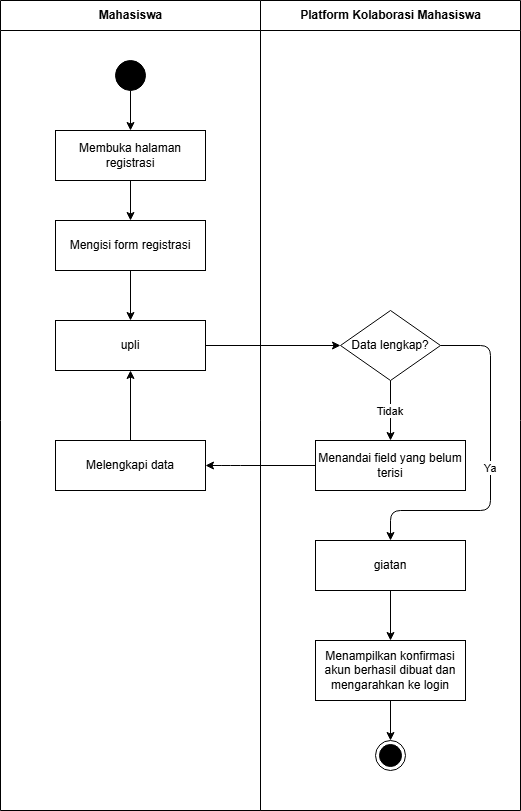
\includegraphics[width=0.9\textwidth,height=0.85\textheight,keepaspectratio]{images/Activity/ActivityUC01.png}
  \caption{\emph{Activity Diagram} UC01 -- Register}
  \label{fig:activity-uc01}
\end{figure}

\clearpage
\subsubsection{\emph{Activity Diagram} UC02}

\emph{Activity diagram} untuk UC02 terdapat pada Gambar~\ref{fig:activity-uc02} berikut.

\begin{figure}[H]
  \centering
  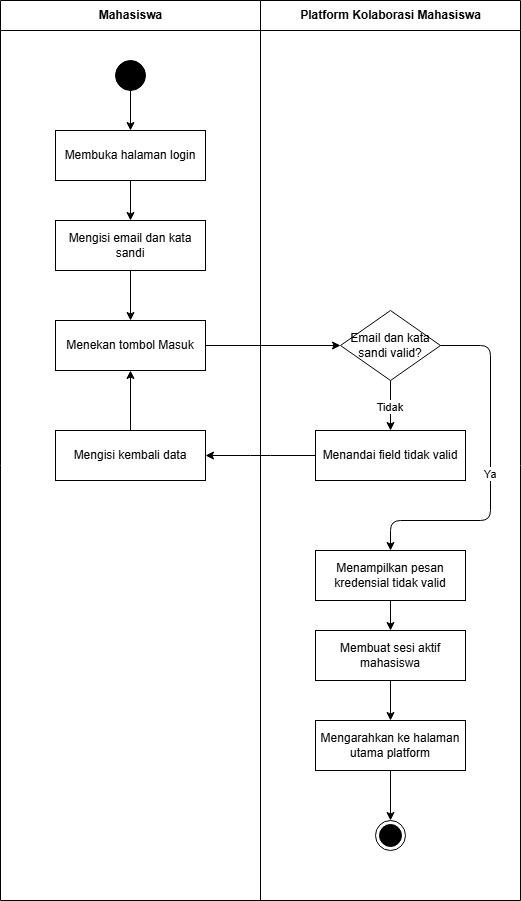
\includegraphics[width=0.9\textwidth,height=0.85\textheight,keepaspectratio]{images/Activity/AcitivityUC02.png}
  \caption{\emph{Activity Diagram} UC02 -- \emph{Login}}
  \label{fig:activity-uc02}
\end{figure}

\clearpage
\subsubsection{\emph{Activity Diagram} UC03}

\emph{Activity diagram} untuk UC03 terdapat pada Gambar~\ref{fig:activity-uc03} berikut.

\begin{figure}[H]
  \centering
  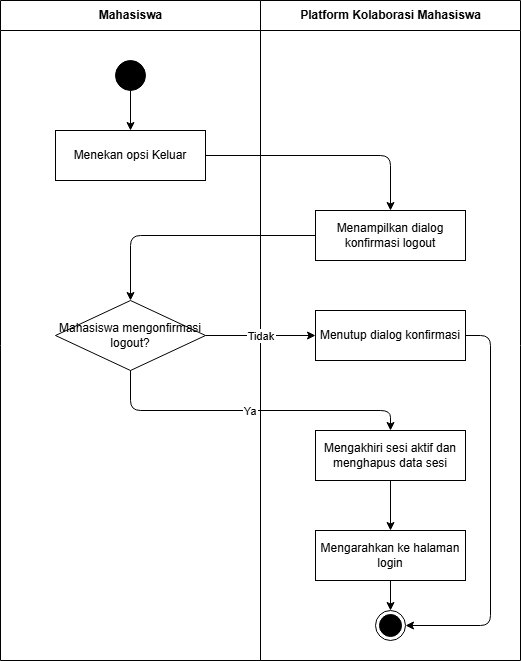
\includegraphics[width=0.9\textwidth,height=0.85\textheight,keepaspectratio]{images/Activity/ActivityUC03.png}
  \caption{\emph{Activity Diagram} UC03 -- \emph{Logout}}
  \label{fig:activity-uc03}
\end{figure}

\clearpage
\subsubsection{\emph{Activity Diagram} UC04}

\emph{Activity diagram} untuk UC04 terdapat pada Gambar~\ref{fig:activity-uc04} berikut.

\begin{figure}[H]
  \centering
  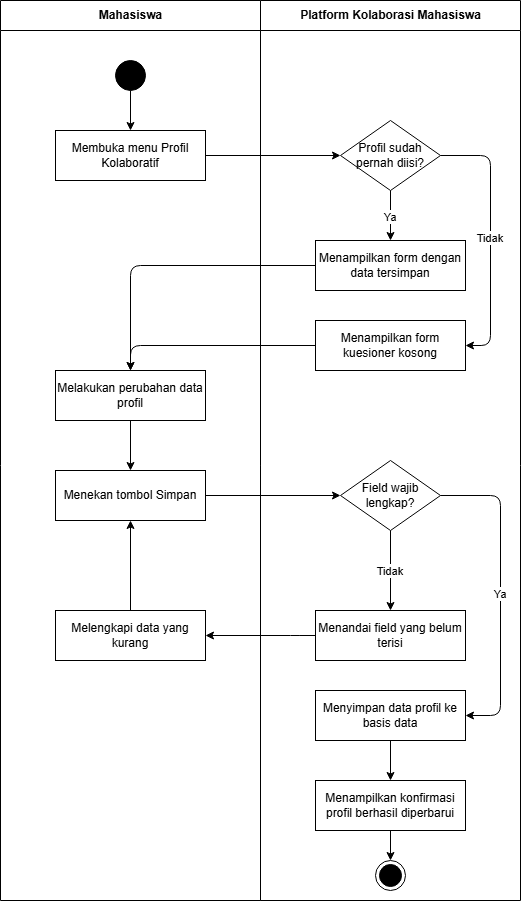
\includegraphics[width=0.9\textwidth,height=0.85\textheight,keepaspectratio]{images/Activity/ActivityUC04.png}
  \caption{\emph{Activity Diagram} UC04 -- Mengelola Profil Kolaboratif}
  \label{fig:activity-uc04}
\end{figure}

\clearpage
\subsubsection{\emph{Activity Diagram} UC05}

\emph{Activity diagram} untuk UC05 terdapat pada Gambar~\ref{fig:activity-uc05} berikut.

\begin{figure}[H]
  \centering
  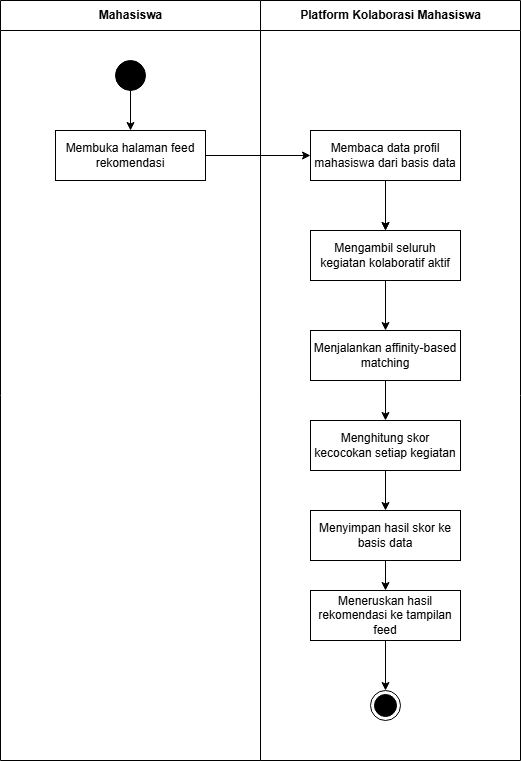
\includegraphics[width=0.9\textwidth,height=0.85\textheight,keepaspectratio]{images/Activity/ActivityUC05.png}
  \caption{\emph{Activity Diagram} UC05 -- Melakukan Pencocokan Rekomendasi}
  \label{fig:activity-uc05}
\end{figure}

\clearpage
\subsubsection{\emph{Activity Diagram} UC06}

\emph{Activity diagram} untuk UC06 terdapat pada Gambar~\ref{fig:activity-uc06} berikut.

\begin{figure}[H]
  \centering
  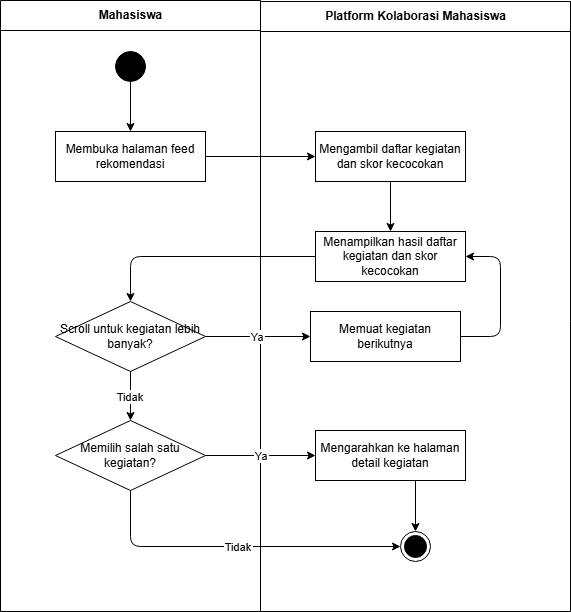
\includegraphics[width=0.9\textwidth,height=0.85\textheight,keepaspectratio]{images/Activity/ActivityUC06.png}
  \caption{\emph{Activity Diagram} UC06 -- Melihat \emph{Feed} Rekomendasi Kegiatan}
  \label{fig:activity-uc06}
\end{figure}

\clearpage
\subsubsection{\emph{Activity Diagram} UC07}

\emph{Activity diagram} untuk UC07 terdapat pada Gambar~\ref{fig:activity-uc07} berikut.

\begin{figure}[H]
  \centering
  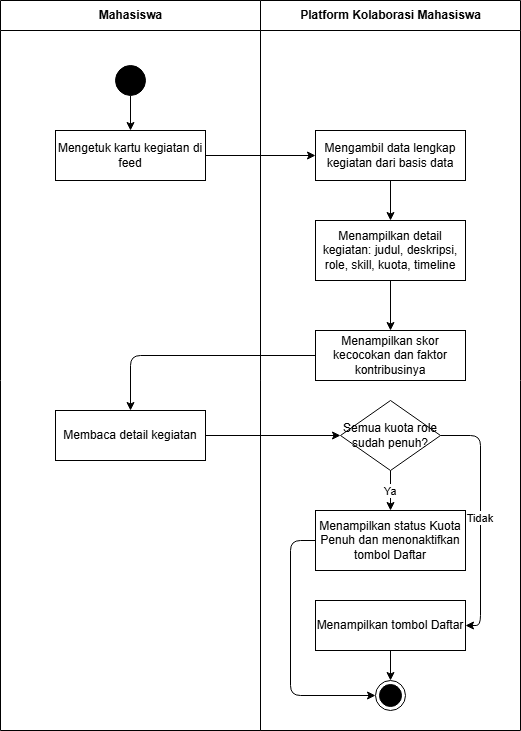
\includegraphics[width=0.9\textwidth,height=0.85\textheight,keepaspectratio]{images/Activity/ActivityUC07.png}
  \caption{\emph{Activity Diagram} UC07 -- Melihat Detail Kegiatan Kolaboratif}
  \label{fig:activity-uc07}
\end{figure}

\clearpage
\subsubsection{\emph{Activity Diagram} UC08}

\emph{Activity diagram} untuk UC08 terdapat pada Gambar~\ref{fig:activity-uc08} berikut.

\begin{figure}[H]
  \centering
  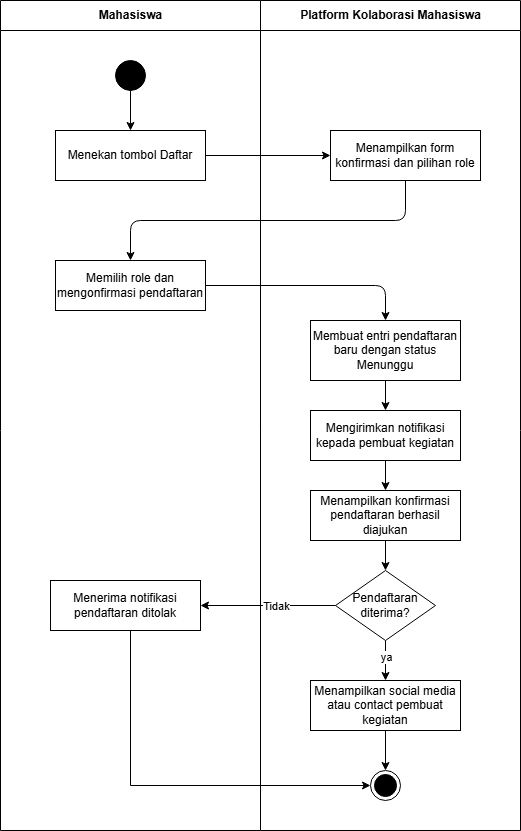
\includegraphics[width=0.9\textwidth,height=0.85\textheight,keepaspectratio]{images/Activity/ActivityUC08.png}
  \caption{\emph{Activity Diagram} UC08 -- Mendaftar ke Kegiatan Kolaboratif}
  \label{fig:activity-uc08}
\end{figure}

\clearpage
\subsubsection{\emph{Activity Diagram} UC09}

\emph{Activity diagram} untuk UC09 terdapat pada Gambar~\ref{fig:activity-uc09} berikut.

\begin{figure}[H]
  \centering
  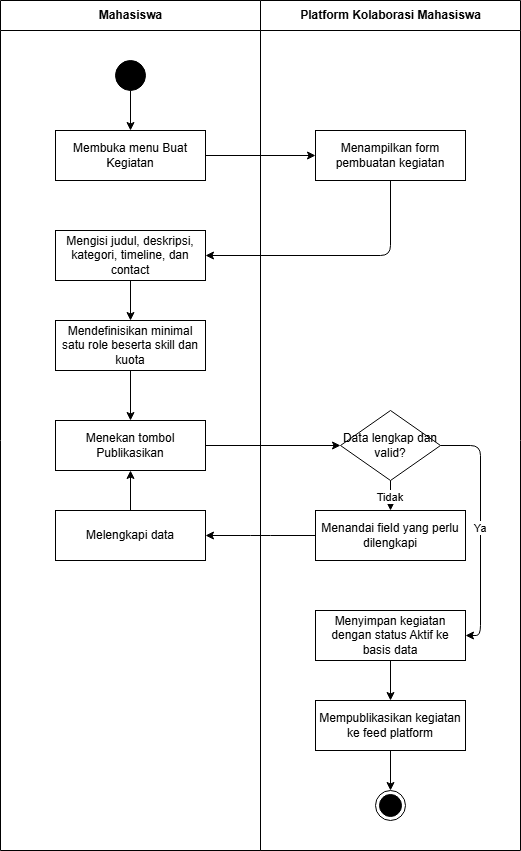
\includegraphics[width=0.9\textwidth,height=0.85\textheight,keepaspectratio]{images/Activity/ActivityUC09.png}
  \caption{\emph{Activity Diagram} UC09 -- Membuat Kegiatan Kolaboratif}
  \label{fig:activity-uc09}
\end{figure}

\clearpage
\subsubsection{\emph{Activity Diagram} UC10}

\emph{Activity diagram} untuk UC10 terdapat pada Gambar~\ref{fig:activity-uc10} berikut.

\begin{figure}[H]
  \centering
  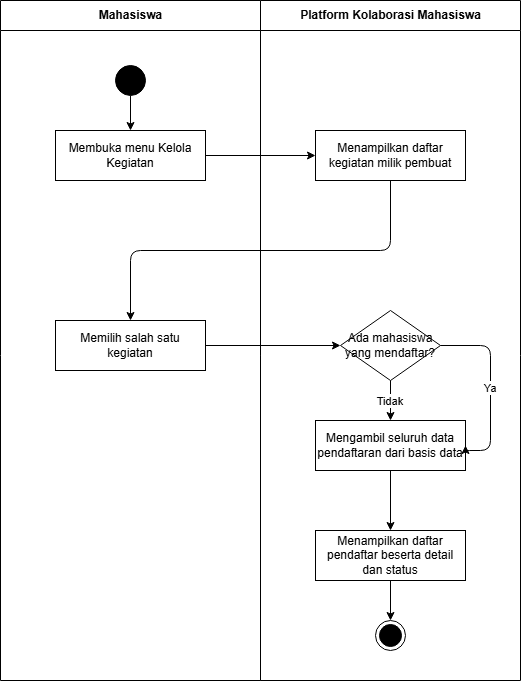
\includegraphics[width=0.9\textwidth,height=0.85\textheight,keepaspectratio]{images/Activity/ActivityUC10.png}
  \caption{\emph{Activity Diagram} UC10 -- Melihat List Pendaftar}
  \label{fig:activity-uc10}
\end{figure}

\clearpage
\subsubsection{\emph{Activity Diagram} UC11}

\emph{Activity diagram} untuk UC11 terdapat pada Gambar~\ref{fig:activity-uc11} berikut.

\begin{figure}[H]
  \centering
  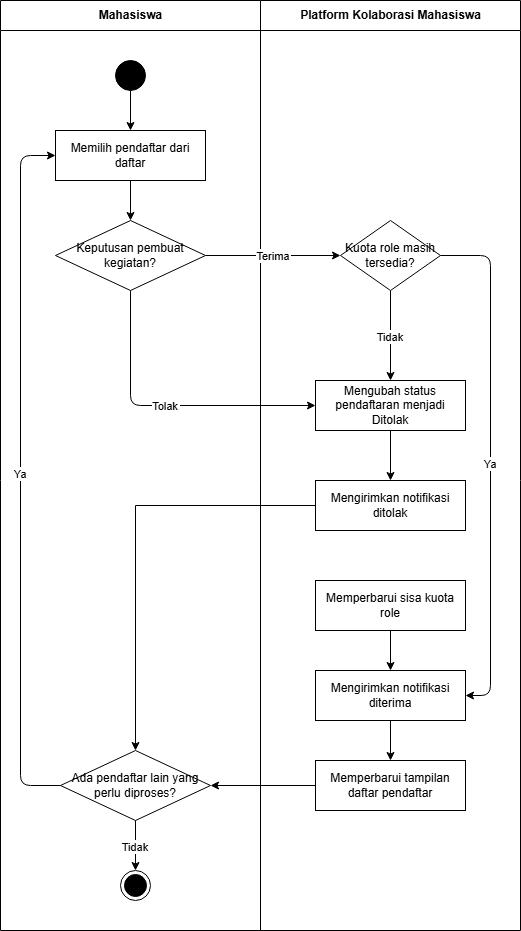
\includegraphics[width=0.9\textwidth,height=0.85\textheight,keepaspectratio]{images/Activity/ActivityUC11.png}
  \caption{\emph{Activity Diagram} UC11 -- Memproses Pendaftaran}
  \label{fig:activity-uc11}
\end{figure}

% ==========================================
\subsection{\emph{Conceptual Class Diagram}}

\emph{Conceptual Class Diagram} digunakan untuk mengidentifikasi kelas-kelas utama yang terdapat pada modul, atribut yang dimiliki oleh setiap kelas, \emph{method}, serta hubungan antarkelas yang merepresentasikan kebutuhan informasi dalam sistem. Melalui pemodelan ini, struktur data yang mendukung fungsi-fungsi pada modul dapat dipahami secara lebih jelas dan menjadi dasar dalam perancangan basis data maupun implementasi sistem. \emph{Conceptual Class Diagram} pada modul \emph{People-to-Project} ditunjukkan pada Gambar~\ref{fig:class-diagram} berikut.

\begin{figure}[H]
  \centering
  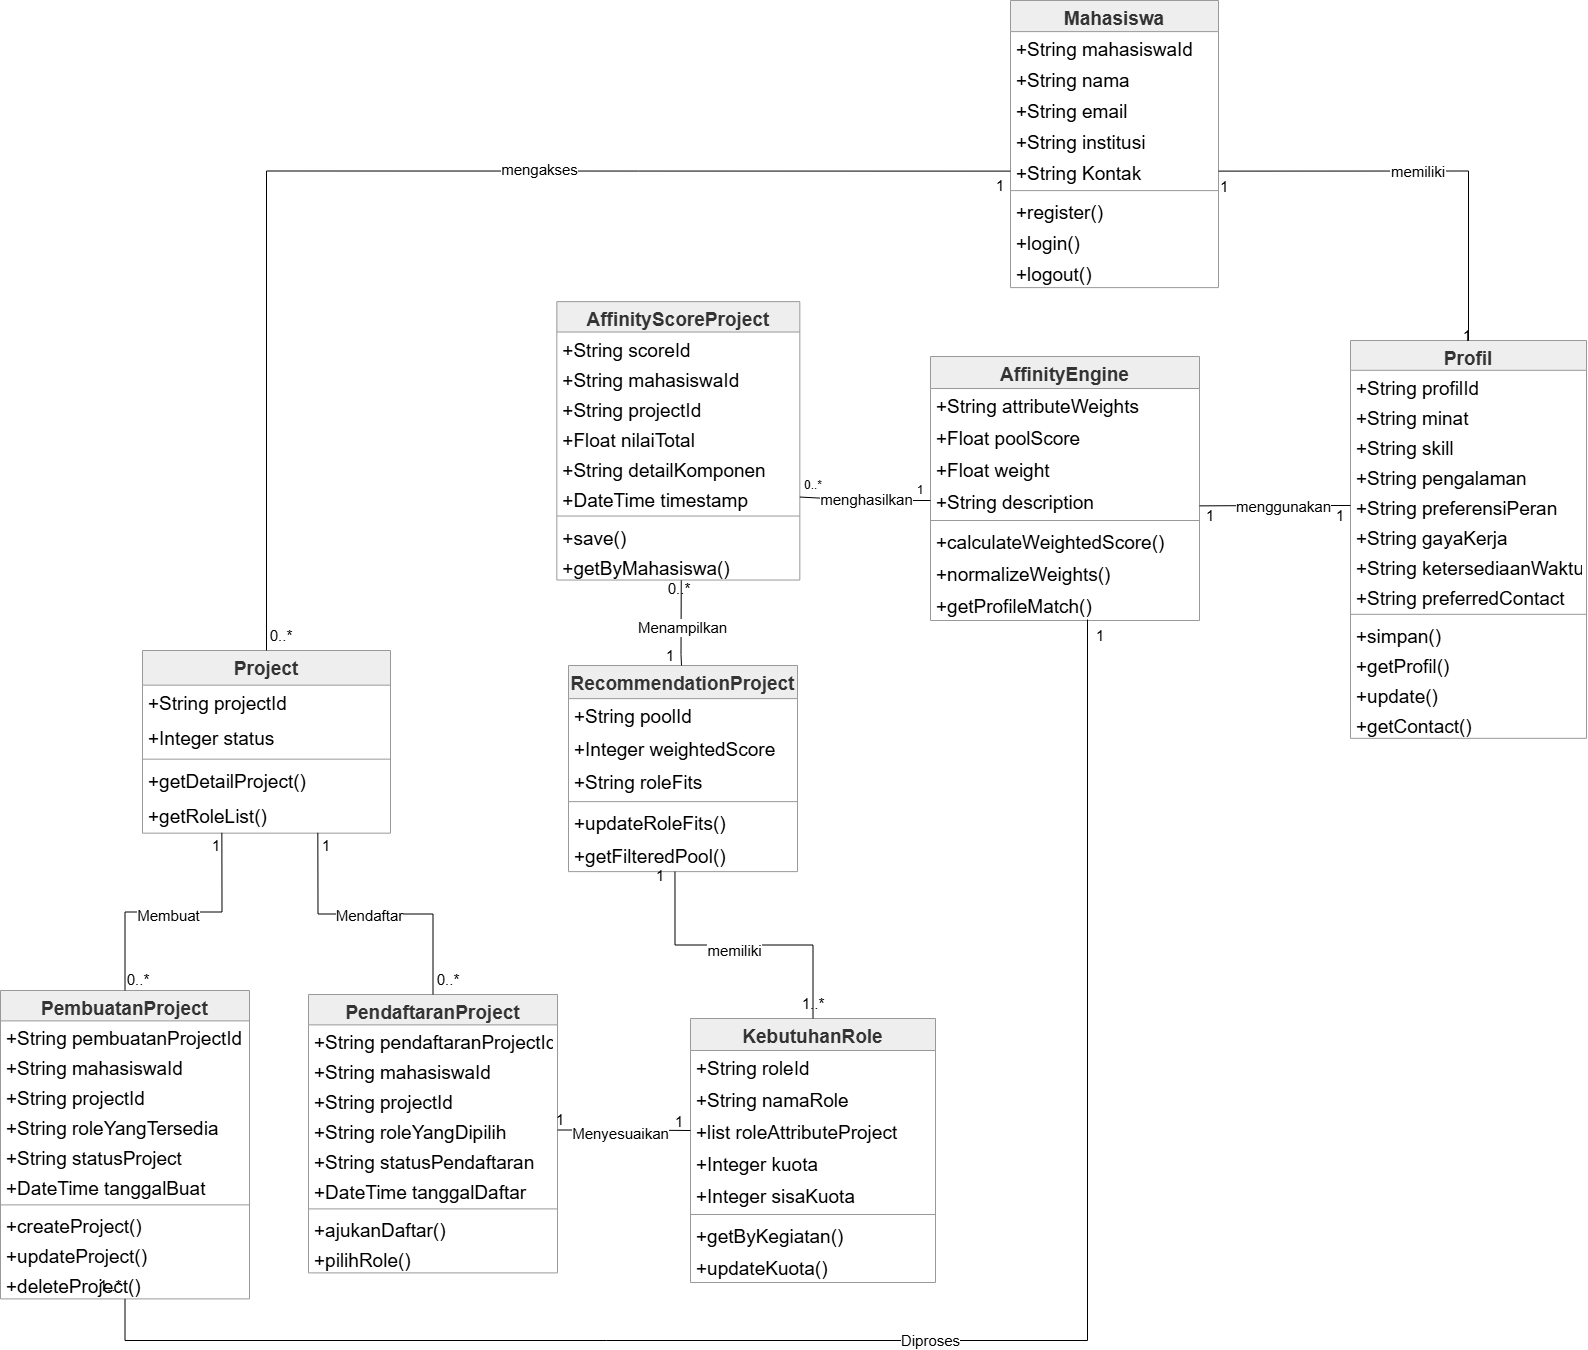
\includegraphics[width=\textwidth]{images/classdiagram.png}
  \caption{\emph{Conceptual Class Diagram} Modul \emph{People-to-Project}}
  \label{fig:class-diagram}
\end{figure}

\emph{Conceptual Class Diagram} di atas menggambarkan sembilan kelas utama yang membentuk struktur data modul \emph{People-to-Project}. Kelas \emph{Mahasiswa} merepresentasikan pengguna sistem dengan atribut identitas dasar beserta operasi autentikasi, dan berelasi satu-ke-satu dengan kelas \emph{Profil} yang menyimpan data kolaboratif meliputi minat, \emph{skill}, pengalaman, preferensi peran, gaya kerja, dan ketersediaan waktu. Data profil ini menjadi masukan utama bagi kelas \emph{AffinityEngine} yang menjalankan mekanisme pencocokan berbasis pembobotan atribut. Hasil perhitungan \emph{AffinityEngine} disimpan pada kelas \emph{AffinityScoreProject} yang merekam skor kecocokan antara mahasiswa dengan setiap \emph{project}, kemudian ditampilkan melalui kelas \emph{RecommendationProject} sebagai kumpulan rekomendasi terfilter.

% ==========================================
\subsection{\emph{Sequence Diagram}}

\emph{Sequence Diagram} digunakan untuk menggambarkan urutan dan interaksi yang terjadi antara aktor, antarmuka sistem, objek kontrol, serta entitas data dalam menjalankan suatu fungsi. Dengan \emph{sequence diagram}, alur eksekusi setiap \emph{use case} dapat divisualisasikan secara lebih rinci sehingga hubungan antarkomponen sistem dan proses pertukaran data dapat dipahami dengan lebih jelas. \emph{Sequence Diagram} untuk \emph{use case} masing-masing pada modul \emph{People-to-Project} disajikan pada gambar-gambar berikut.

\subsubsection{\emph{Sequence Diagram} UC01}

\emph{Sequence diagram} untuk UC01 terdapat pada Gambar~\ref{fig:sequence-uc01} berikut.

\begin{figure}[H]
  \centering
  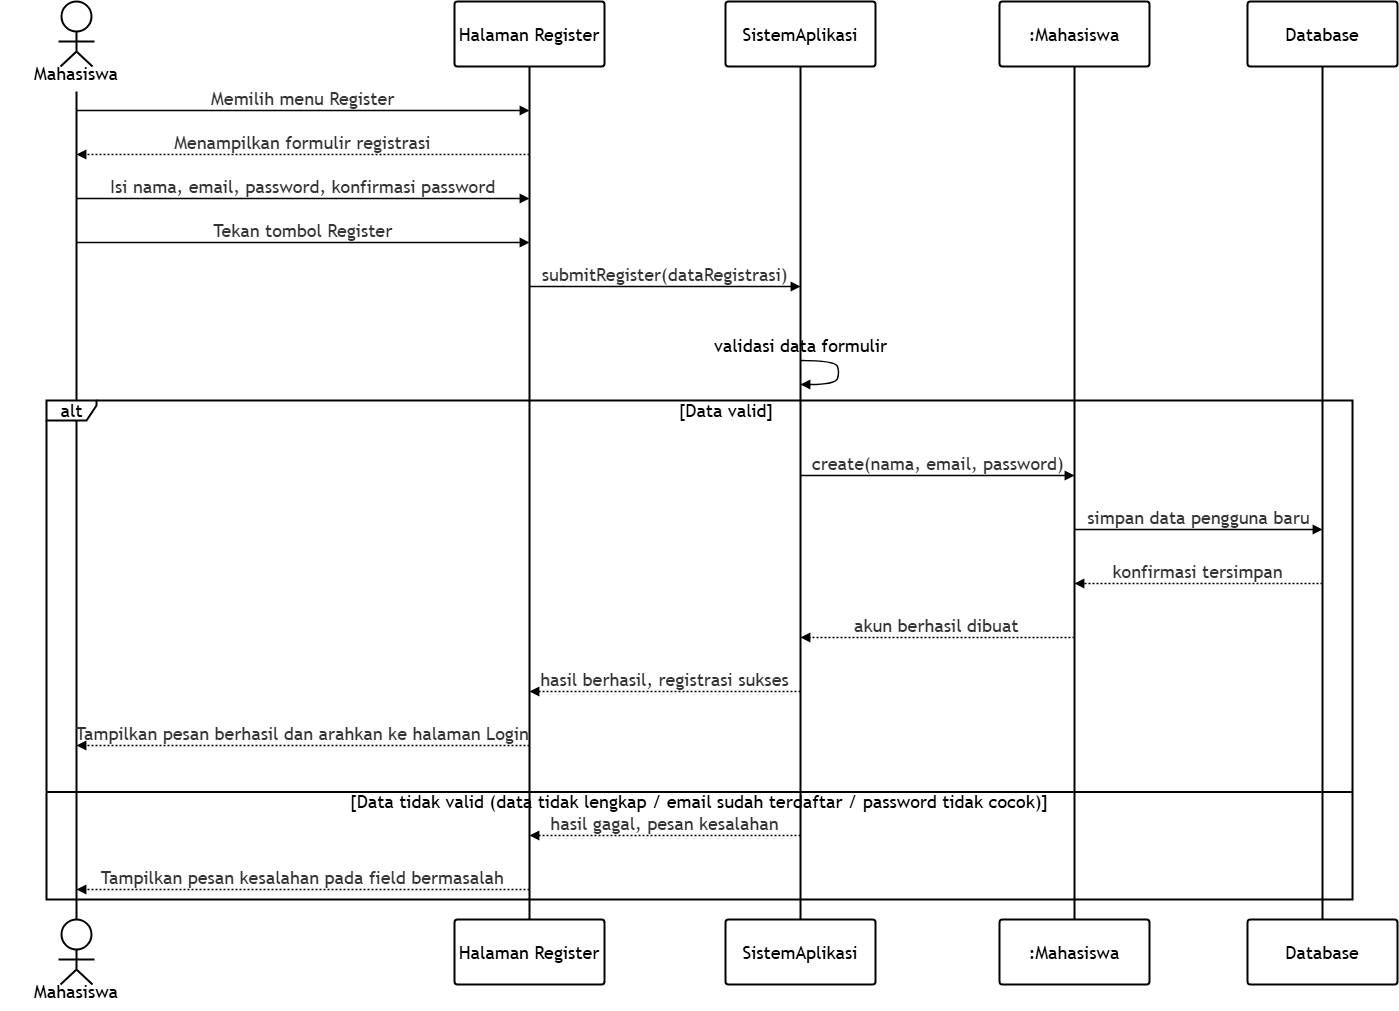
\includegraphics[width=\textwidth]{images/Sequence/SequenceUC01.png}
  \caption{\emph{Sequence Diagram} UC01 -- Register}
  \label{fig:sequence-uc01}
\end{figure}

\subsubsection{\emph{Sequence Diagram} UC02}

\emph{Sequence diagram} untuk UC02 terdapat pada Gambar~\ref{fig:sequence-uc02} berikut.

\begin{figure}[H]
  \centering
  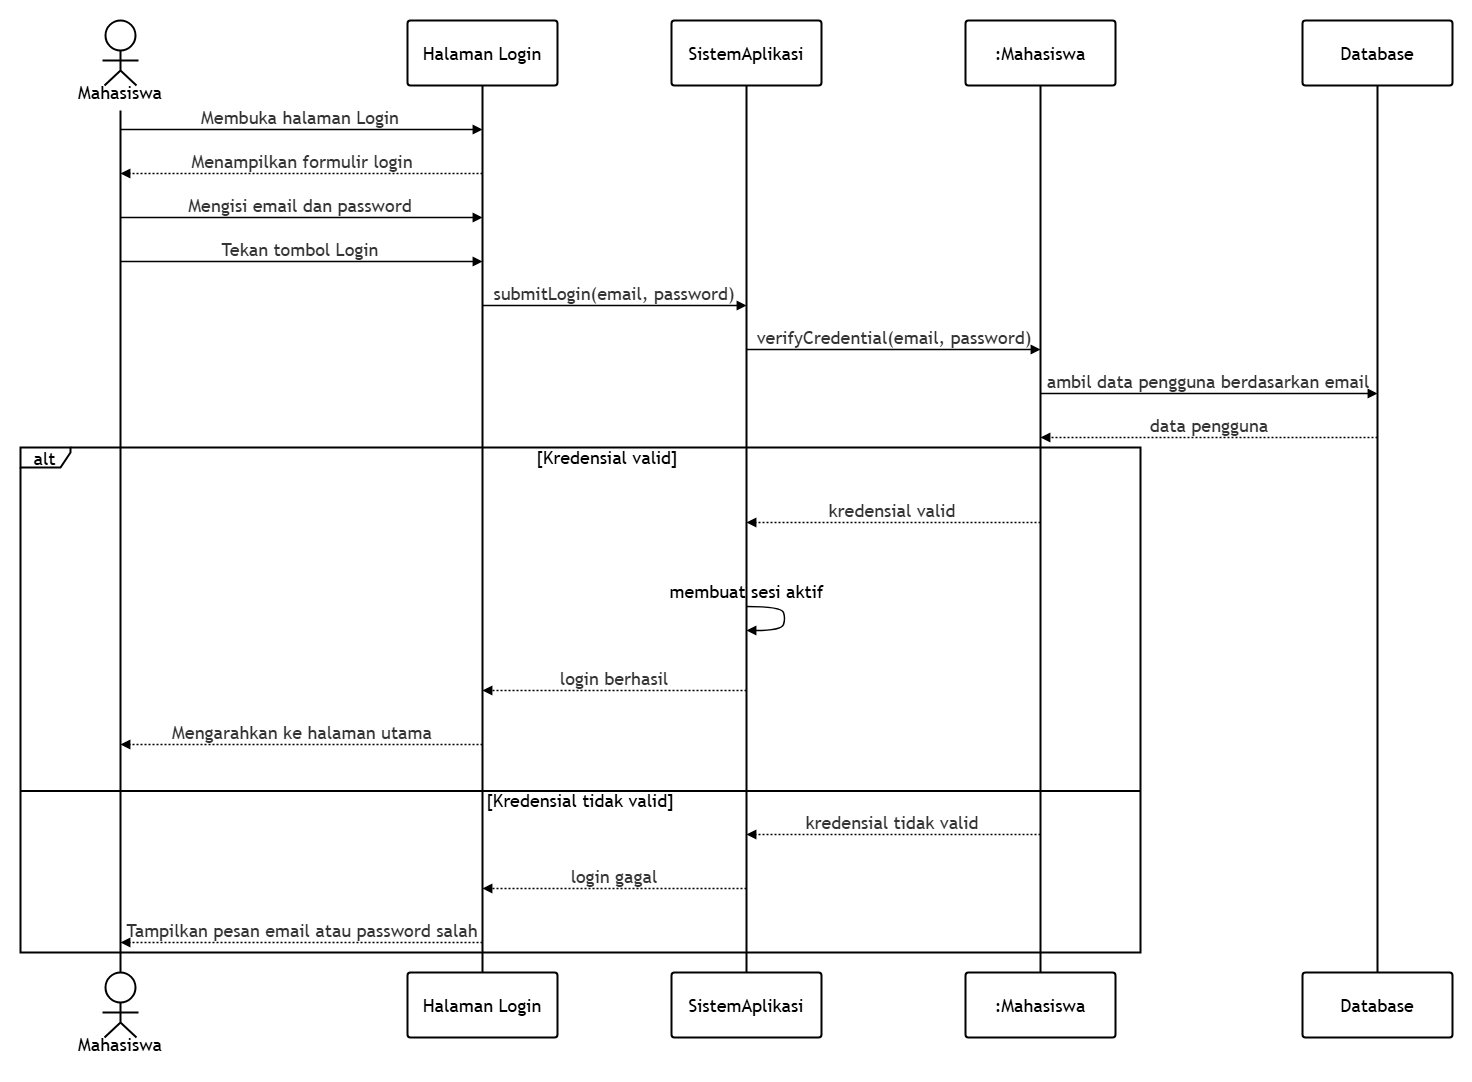
\includegraphics[width=\textwidth]{images/Sequence/SequenceUC02.png}
  \caption{\emph{Sequence Diagram} UC02 -- \emph{Login}}
  \label{fig:sequence-uc02}
\end{figure}

\subsubsection{\emph{Sequence Diagram} UC03}

\emph{Sequence diagram} untuk UC03 terdapat pada Gambar~\ref{fig:sequence-uc03} berikut.

\begin{figure}[H]
  \centering
  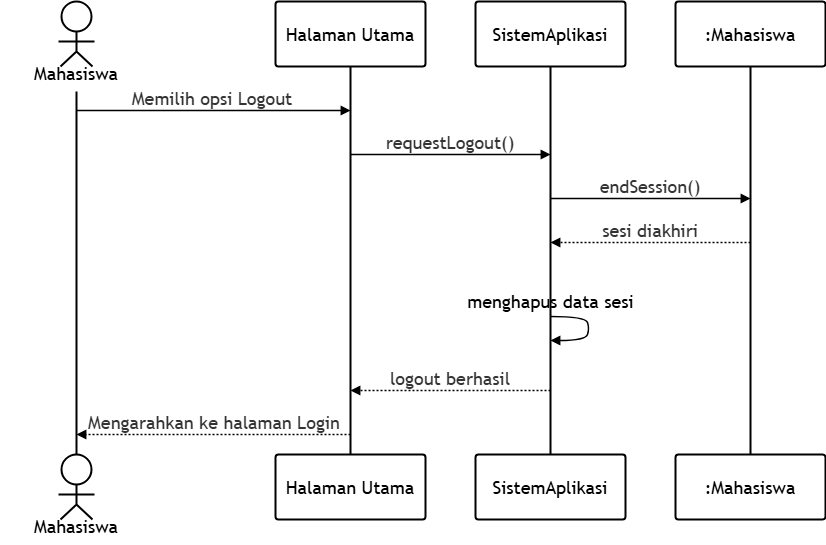
\includegraphics[width=\textwidth]{images/Sequence/SequenceUC03.png}
  \caption{\emph{Sequence Diagram} UC03 -- \emph{Logout}}
  \label{fig:sequence-uc03}
\end{figure}

\subsubsection{\emph{Sequence Diagram} UC04}

\emph{Sequence diagram} untuk UC04 terdapat pada Gambar~\ref{fig:sequence-uc04} berikut.

\begin{figure}[H]
  \centering
  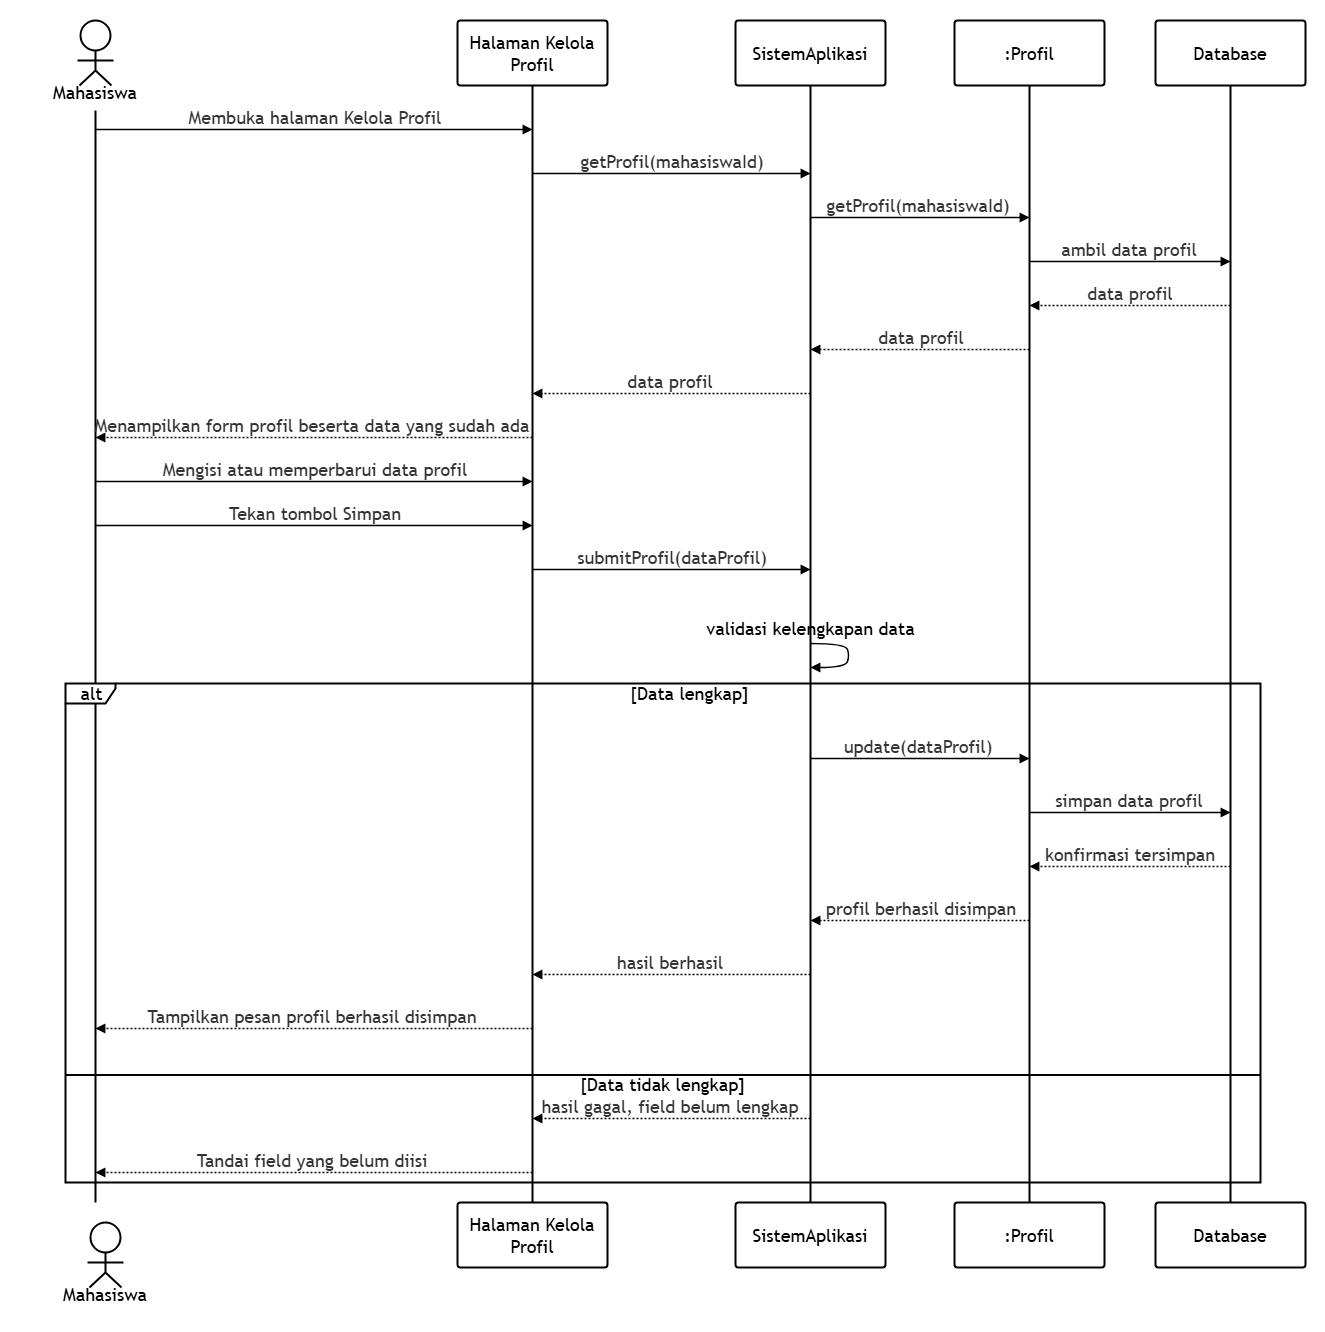
\includegraphics[width=\textwidth]{images/Sequence/SequenceUC04.png}
  \caption{\emph{Sequence Diagram} UC04 -- Mengelola Profil Kolaboratif}
  \label{fig:sequence-uc04}
\end{figure}

\subsubsection{\emph{Sequence Diagram} UC05}

\emph{Sequence diagram} untuk UC05 terdapat pada Gambar~\ref{fig:sequence-uc05} berikut.

\begin{figure}[H]
  \centering
  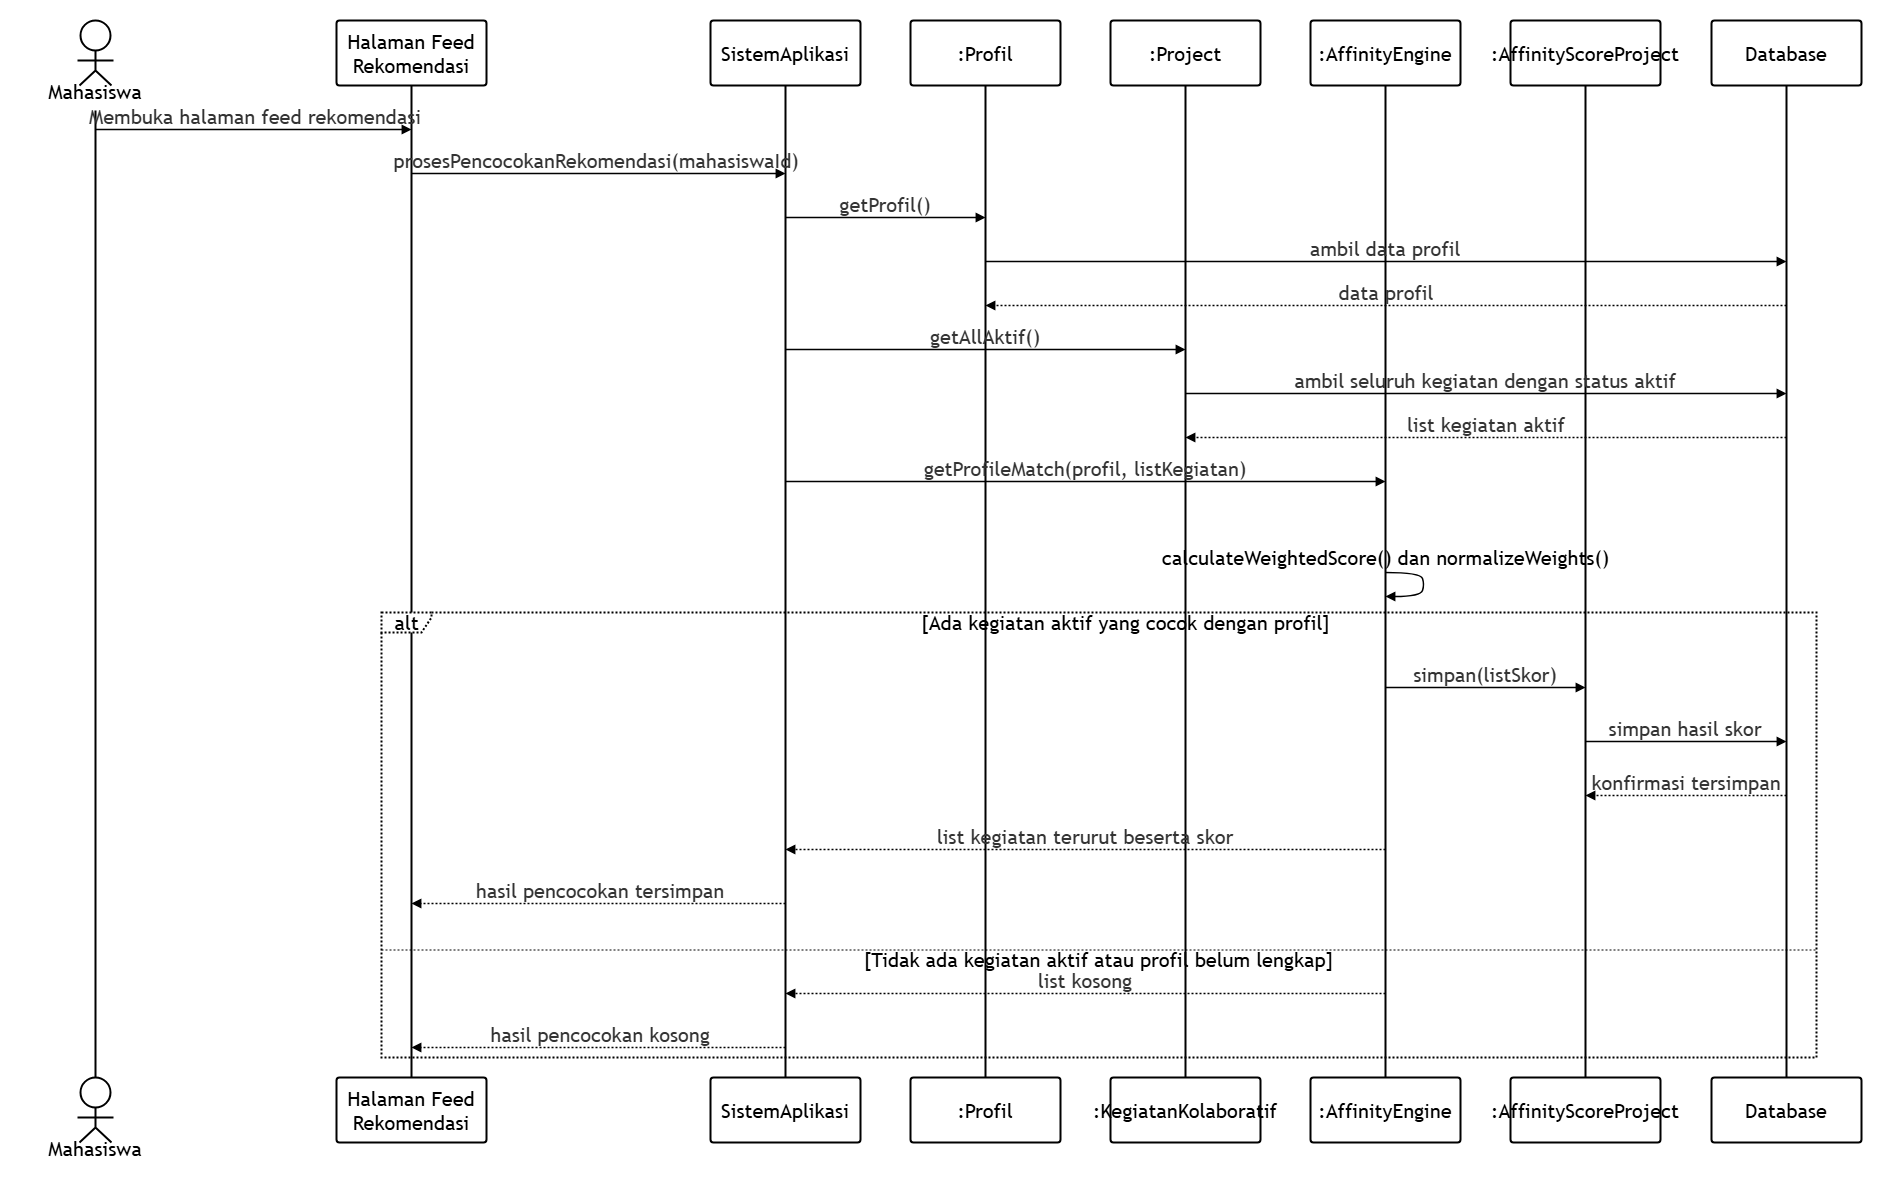
\includegraphics[width=\textwidth]{images/Sequence/SequenceUC05.png}
  \caption{\emph{Sequence Diagram} UC05 -- Melakukan Pencocokan Rekomendasi}
  \label{fig:sequence-uc05}
\end{figure}

\subsubsection{\emph{Sequence Diagram} UC06}

\emph{Sequence diagram} untuk UC06 terdapat pada Gambar~\ref{fig:sequence-uc06} berikut.

\begin{figure}[H]
  \centering
  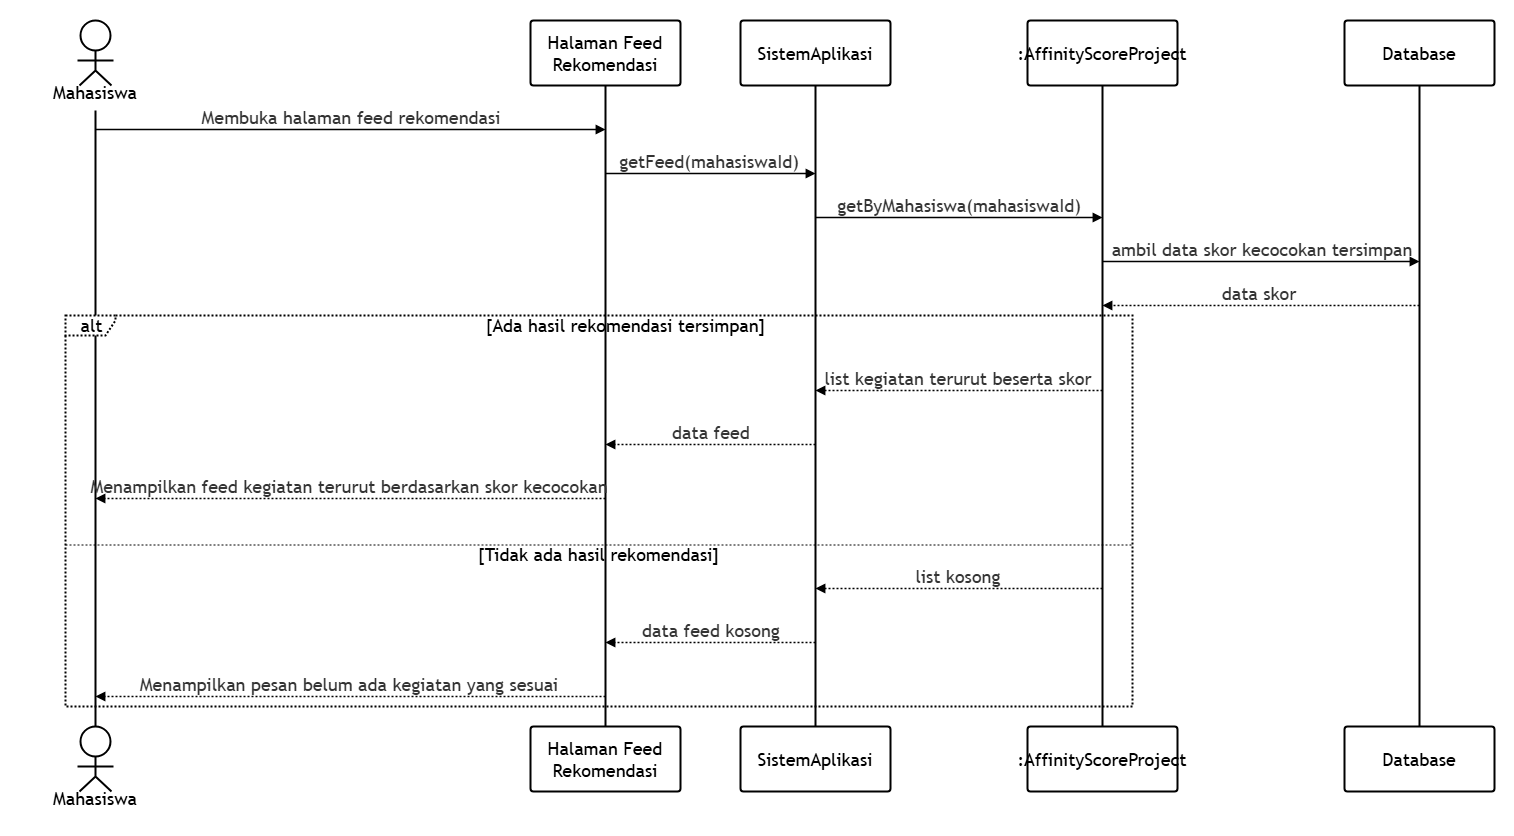
\includegraphics[width=\textwidth]{images/Sequence/SequenceUC06.png}
  \caption{\emph{Sequence Diagram} UC06 -- Melihat \emph{Feed} Rekomendasi Kegiatan}
  \label{fig:sequence-uc06}
\end{figure}

\subsubsection{\emph{Sequence Diagram} UC07}

\emph{Sequence diagram} untuk UC07 terdapat pada Gambar~\ref{fig:sequence-uc07} berikut.

\begin{figure}[H]
  \centering
  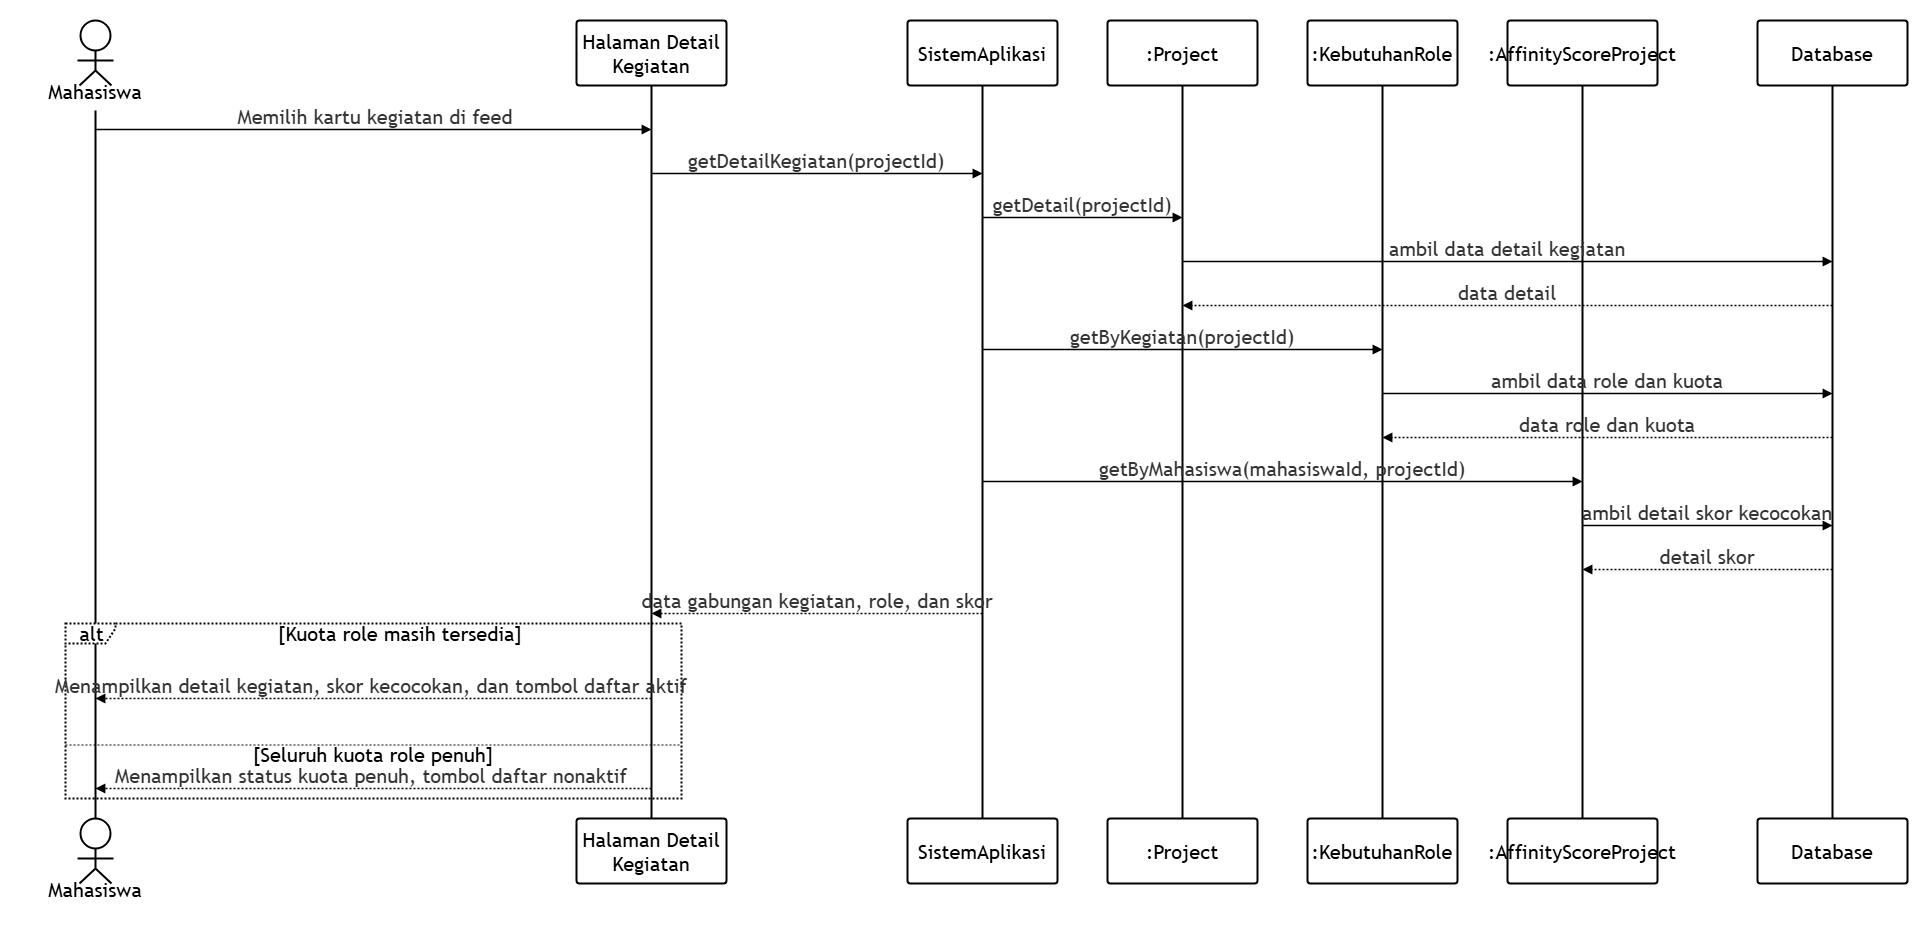
\includegraphics[width=\textwidth]{images/Sequence/SequenceUC07.png}
  \caption{\emph{Sequence Diagram} UC07 -- Melihat Detail Kegiatan Kolaboratif}
  \label{fig:sequence-uc07}
\end{figure}

\subsubsection{\emph{Sequence Diagram} UC08}

\emph{Sequence diagram} untuk UC08 terdapat pada Gambar~\ref{fig:sequence-uc08} berikut.

\begin{figure}[H]
  \centering
  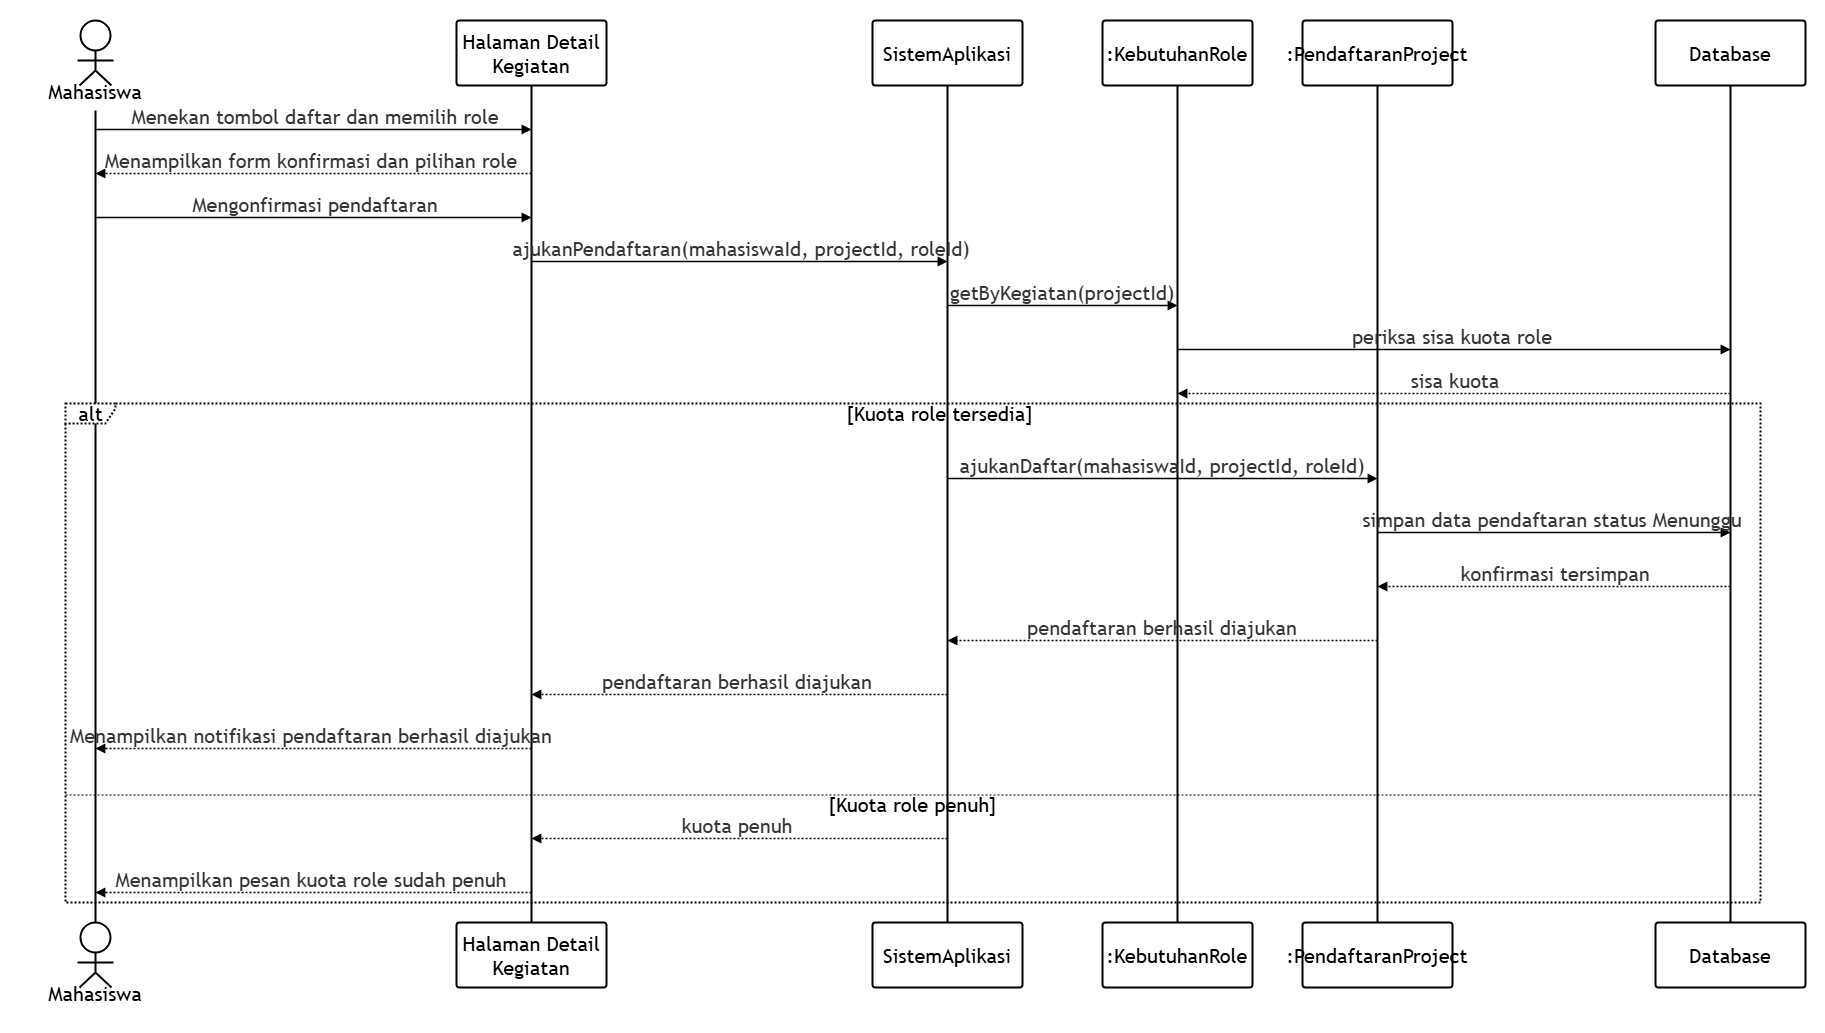
\includegraphics[width=\textwidth]{images/Sequence/SequenceUC08.png}
  \caption{\emph{Sequence Diagram} UC08 -- Mendaftar ke Kegiatan Kolaboratif}
  \label{fig:sequence-uc08}
\end{figure}

\subsubsection{\emph{Sequence Diagram} UC09}

\emph{Sequence diagram} untuk UC09 terdapat pada Gambar~\ref{fig:sequence-uc09} berikut.

\begin{figure}[H]
  \centering
  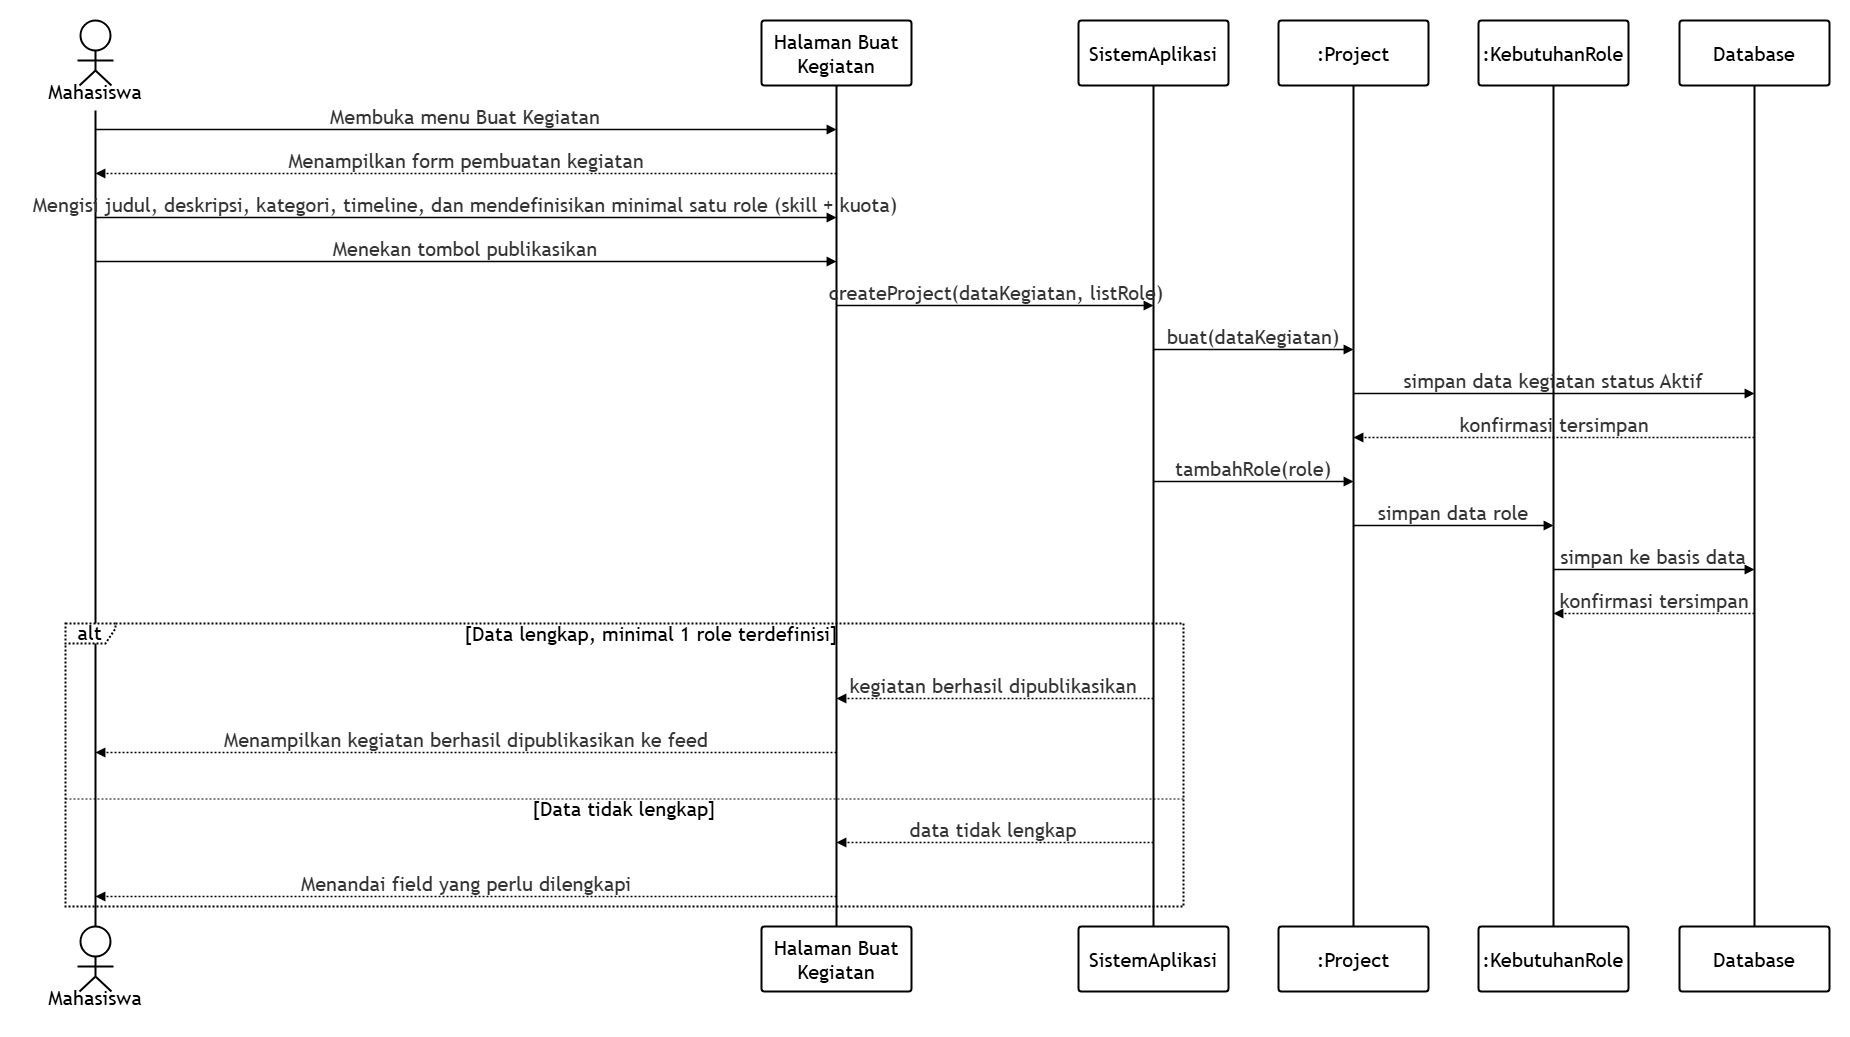
\includegraphics[width=\textwidth]{images/Sequence/SequenceUC09.png}
  \caption{\emph{Sequence Diagram} UC09 -- Membuat Kegiatan Kolaboratif}
  \label{fig:sequence-uc09}
\end{figure}

\subsubsection{\emph{Sequence Diagram} UC10}

\emph{Sequence diagram} untuk UC10 terdapat pada Gambar~\ref{fig:sequence-uc10} berikut.

\begin{figure}[H]
  \centering
  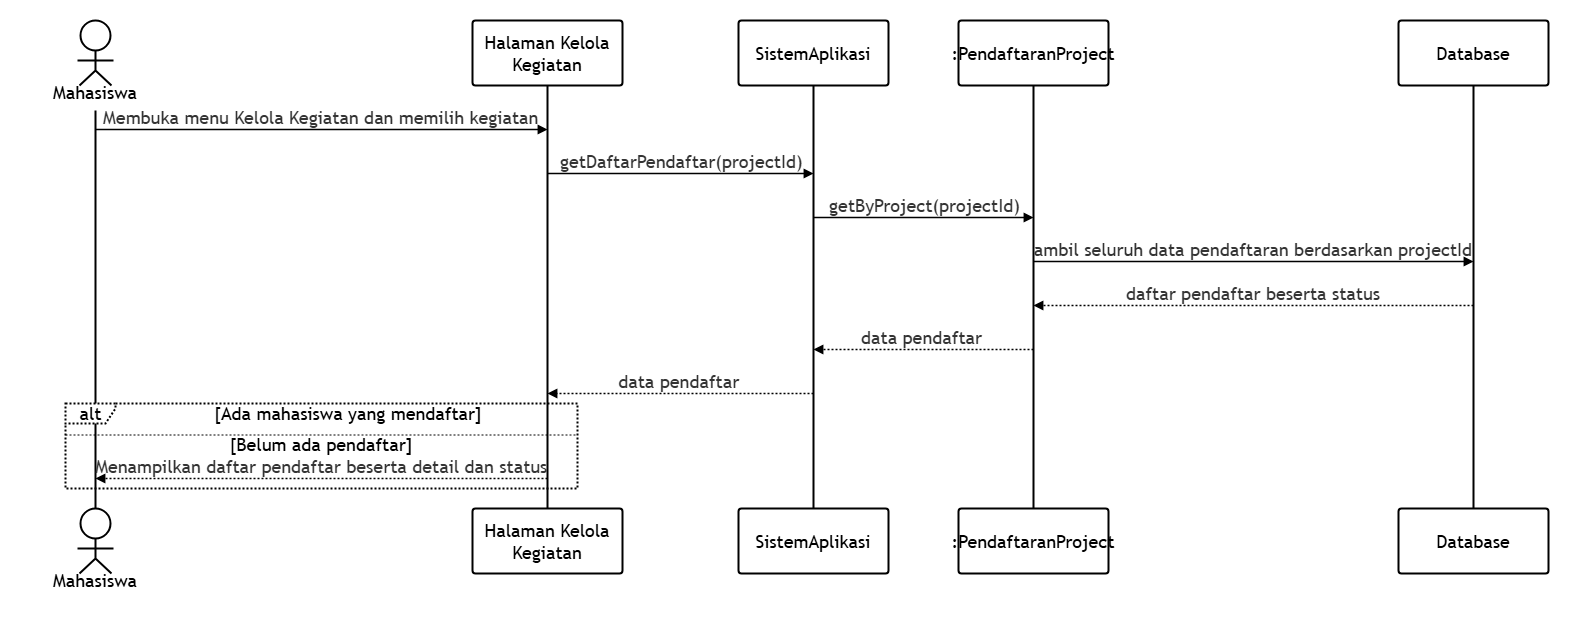
\includegraphics[width=\textwidth]{images/Sequence/SequenceUC10.png}
  \caption{\emph{Sequence Diagram} UC10 -- Melihat List Pendaftar}
  \label{fig:sequence-uc10}
\end{figure}

\subsubsection{\emph{Sequence Diagram} UC11}

\emph{Sequence diagram} untuk UC11 terdapat pada Gambar~\ref{fig:sequence-uc11} berikut.

\begin{figure}[H]
  \centering
  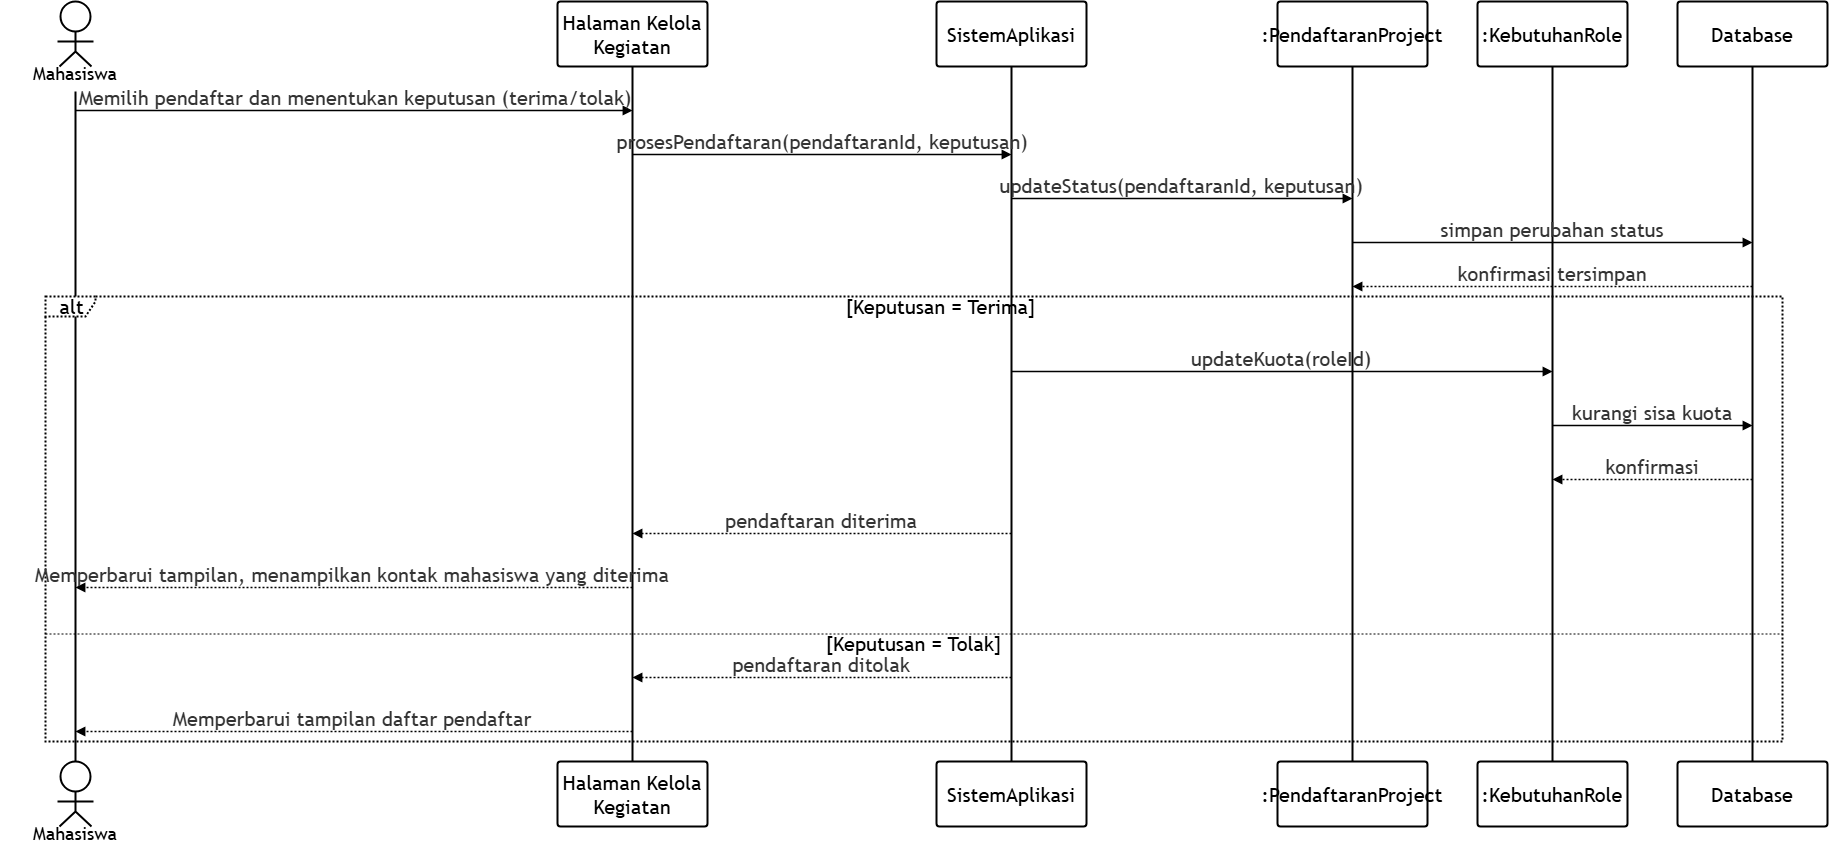
\includegraphics[width=\textwidth]{images/Sequence/SequenceUC11.png}
  \caption{\emph{Sequence Diagram} UC11 -- Memproses Pendaftaran}
  \label{fig:sequence-uc11}
\end{figure}

% ==========================================
\subsection{\emph{Component Diagram}}

Subsistem \emph{People-to-Project} dirancang ke dalam tiga \emph{component}, yaitu RekomendasiFeedProject, PembuatanProject, dan PendaftaranProject. Pengelompokan ini dilakukan berdasarkan kesamaan tanggung jawab (\emph{cohesion}) antarkelas, serta meminimalkan ketergantungan yang tidak perlu antar-\emph{component} (\emph{coupling}), mengikuti prinsip perancangan arsitektur berorientasi \emph{component} \autocite{sommerville2016}. Gambar~\ref{fig:component-diagram} menunjukkan struktur internal ketiga \emph{component} tersebut, beserta interaksinya dengan subsistem General Features yang menyediakan fungsi lintas modul berupa pengelolaan akun, mesin pencocokan, dan layanan notifikasi. Setiap hubungan digambarkan melalui \emph{port}, \emph{provided interface}, dan \emph{required interface}, untuk menunjukkan secara eksplisit \emph{component} mana yang menyediakan suatu kemampuan dan \emph{component} mana yang memanfaatkannya.

\begin{figure}[H]
  \centering
  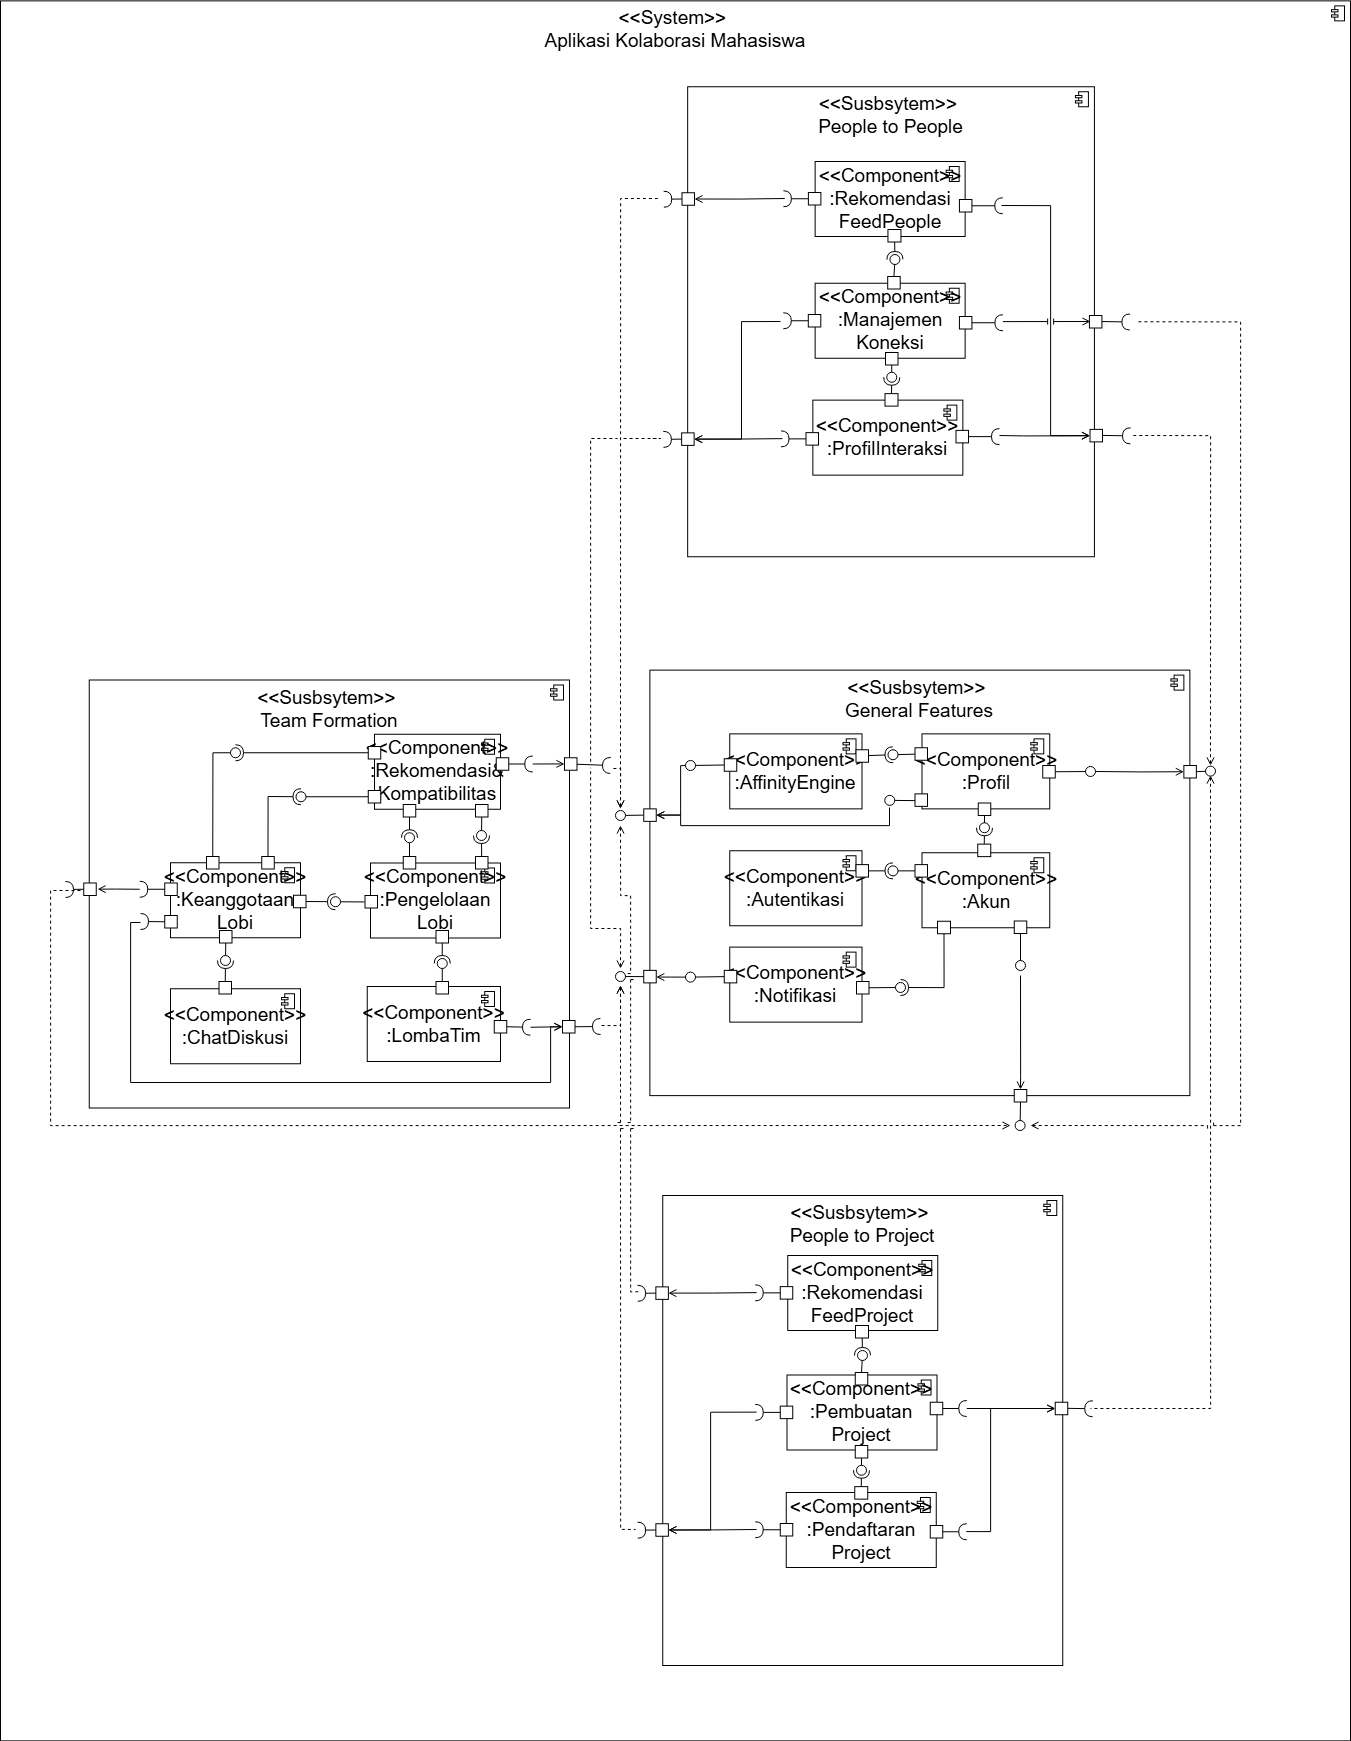
\includegraphics[width=\textwidth]{images/componentdiagram.png}
  \caption{\emph{Component Diagram} Platform Kolaborasi Mahasiswa}
  \label{fig:component-diagram}
\end{figure}

Berdasarkan \emph{component diagram} pada Gambar~\ref{fig:component-diagram}, seluruh hubungan antarkomponen internal pada modul \emph{People-to-Project} bersifat satu arah (\emph{directional}). Tidak ditemukan adanya pasangan komponen dengan hubungan dua arah maupun hubungan siklis (\emph{circular dependency}) di dalam modul ini sehingga setiap komponen dapat diuji, dikembangkan, dan dimutasi secara independen dengan tingkat \emph{coupling} yang sangat rendah. Hubungan luar dari modul ini terhubung ke subsistem General Features dan \emph{port} sistem eksternal untuk mendukung fungsionalitas manajemen proyek mahasiswa. Tabel~\ref{tab:component-relations} menunjukkan detail dari hubungan masing-masing pada \emph{component diagram} yang dibuat.

\begin{longtable}{>{\raggedright\arraybackslash}p{3cm} >{\raggedright\arraybackslash}p{2.5cm} >{\raggedright\arraybackslash}p{4cm} >{\raggedright\arraybackslash}p{\dimexpr\linewidth-9.5cm-8\tabcolsep\relax}}
  \caption{Detail Hubungan \emph{Component Diagram}}
  \label{tab:component-relations} \\
  \toprule
  \textbf{\emph{Provided Interface}} & \textbf{Nama Hubungan} & \textbf{\emph{Required Interface}} & \textbf{Deskripsi} \\
  \midrule
  \endfirsthead
  \multicolumn{4}{l}{\small\textit{Tabel~\ref{tab:component-relations} Detail Hubungan \emph{Component Diagram} (lanjutan)}} \\
  \toprule
  \textbf{\emph{Provided Interface}} & \textbf{Nama Hubungan} & \textbf{\emph{Required Interface}} & \textbf{Deskripsi} \\
  \midrule
  \endhead
  \bottomrule
  \multicolumn{4}{r}{\textit{Bersambung ke halaman berikutnya.}} \\
  \endfoot
  \bottomrule
  \endlastfoot
  \multicolumn{4}{l}{\textbf{Antar komponen di dalam \emph{People-to-Project}}} \\
  \midrule
  Pembuatan\hspace{0pt}Project & Akses Fitur Pembuatan & Rekomendasi\hspace{0pt}Feed\hspace{0pt}Project & Komponen \emph{feed} rekomendasi proyek memerlukan layanan/\emph{interface} dari pembuatan proyek untuk mengintegrasikan proyek-proyek baru yang berhasil dibuat ke dalam daftar \emph{feed} pengguna. \\
  \midrule
  Pendaftaran\hspace{0pt}Project & Proses Pendaftaran & Pembuatan\hspace{0pt}Project & Komponen pendaftaran proyek memerlukan pembuatan proyek agar mahasiswa dapat melakukan registrasi atau bergabung ke dalam proyek yang telah valid dibuat. \\
  \midrule
  \multicolumn{4}{l}{\textbf{\emph{People-to-Project} ke General Features}} \\
  \midrule
  Profil (Subsistem General Features), \emph{AffinityEngine} (Subsistem General Features) & Data Personalisasi \emph{Feed} & Rekomendasi\hspace{0pt}Feed\hspace{0pt}Project & Komponen \emph{feed} proyek membutuhkan informasi dari profil mahasiswa dan \emph{AffinityEngine} untuk menyaring dan menampilkan rekomendasi proyek yang paling relevan dengan minat atau \emph{skill} pengguna. \\
  \midrule
  Profil (Subsistem General Features) & Data Identitas Proyek & Pendaftaran\hspace{0pt}Project, Pembuatan\hspace{0pt}Project & Komponen pendaftaran dan pembuatan proyek membutuhkan data dari komponen profil untuk mengidentifikasi mahasiswa yang bertindak sebagai pembuat (\emph{owner}) proyek maupun yang mendaftar ke proyek tersebut. \\
  \midrule
  Notifikasi (Subsistem General Features) & \emph{Alert} \& Pembaruan Status & Pendaftaran\hspace{0pt}Project, Pembuatan\hspace{0pt}Project & Komponen pendaftaran dan pembuatan proyek membutuhkan layanan notifikasi untuk mengirimkan pemberitahuan sistem, seperti proyek berhasil dibuat, pendaftaran berhasil, atau adanya pendaftar baru kepada mahasiswa terkait. \\
\end{longtable}

% ==========================================
\subsection{\emph{Deployment Diagram}}

\emph{Deployment diagram} digunakan untuk menggambarkan konfigurasi perangkat keras (\emph{hardware}) dan perangkat lunak (\emph{software}) yang terlibat dalam implementasi sistem, serta hubungan komunikasi di antara komponen-komponen tersebut. Melalui \emph{deployment diagram}, dapat diketahui bagaimana aplikasi ditempatkan pada lingkungan operasional, bagaimana pengguna mengakses sistem, serta bagaimana data dan layanan diproses selama sistem berjalan. \emph{Deployment Diagram} pada sistem Platform Kolaborasi Mahasiswa ditunjukkan pada Gambar~\ref{fig:deployment-diagram} berikut.

\begin{figure}[H]
  \centering
  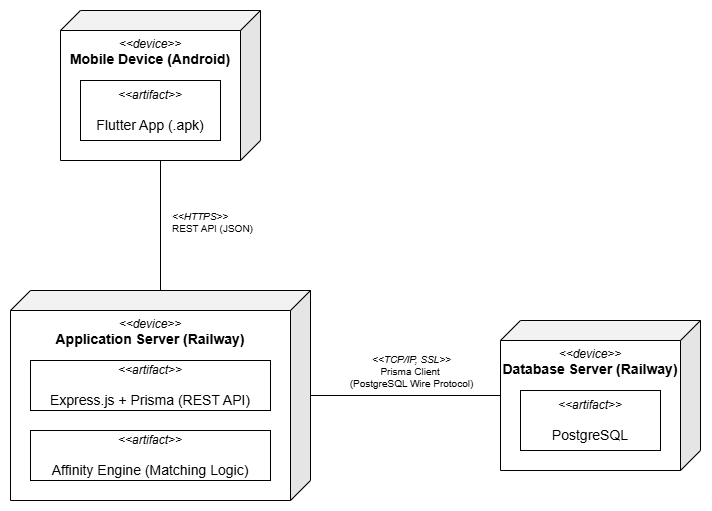
\includegraphics[width=\textwidth]{images/Deploymentdiagram.png}
  \caption{\emph{Deployment Diagram} Platform Kolaborasi Mahasiswa}
  \label{fig:deployment-diagram}
\end{figure}

Sistem terdiri dari tiga \emph{node} utama. \emph{Node} pertama adalah \emph{Mobile Device} (Android) yang menjalankan \emph{artifact} \emph{Flutter App} (.apk), berperan sebagai \emph{presentation layer} yang menangani interaksi pengguna pada modul \emph{People-to-People}, \emph{People-to-Project}, dan \emph{Team Formation} dalam satu basis kode aplikasi. \emph{Node} kedua adalah \emph{Application Server} (Railway) yang menjalankan dua \emph{artifact}: Express.js + Prisma sebagai REST API yang melayani permintaan dari ketiga modul melalui satu \emph{backend} bersama, dan \emph{AffinityEngine} yang memuat logika pembobotan atribut serta perhitungan skor kecocokan yang digunakan bersama oleh ketiga modul, termasuk AffinityScorePeople pada modul ini. \emph{Node} ketiga adalah \emph{Database Server} (Railway) yang menjalankan PostgreSQL Database sebagai satu basis data terpadu yang menyimpan seluruh data sistem, termasuk profil mahasiswa, AffinityScorePeople, RecommendationPeople, SavedProfile, ExpressInterest, ConnectRequest, dan Connection.

Komunikasi antara Mobile Device dan Application Server menggunakan protokol HTTPS dengan format data REST API (JSON), sedangkan komunikasi antara Application Server dan Database Server menggunakan protokol TCP/IP dengan SSL melalui Prisma Client (PostgreSQL Wire Protocol). Application Server dan Database Server di-\emph{deploy} sebagai dua \emph{managed service} terpisah pada platform Railway, sejalan dengan praktik pemisahan basis data dari server aplikasi untuk menjaga keamanan dan isolasi data sebagaimana direkomendasikan dalam arsitektur \emph{client-server} \autocite{sommerville2016}. Rincian \emph{node} dan \emph{artifact} pada \emph{deployment diagram} disajikan pada Tabel~\ref{tab:deployment-nodes}.

\begin{longtable}{p{4cm} p{4cm} >{\raggedright\arraybackslash}p{\dimexpr\linewidth-8cm-6\tabcolsep\relax}}
  \caption{\emph{Node} dan \emph{Artifact} pada \emph{Deployment Diagram}}
  \label{tab:deployment-nodes} \\
  \toprule
    \textbf{\emph{Node}} & \textbf{\emph{Artifact}} & \textbf{Peran} \\
  \midrule
  \endfirsthead
  \multicolumn{3}{l}{\small\textit{Tabel~\ref{tab:deployment-nodes} \emph{Node} dan \emph{Artifact} pada \emph{Deployment Diagram} (lanjutan)}} \\
  \toprule
    \textbf{\emph{Node}} & \textbf{\emph{Artifact}} & \textbf{Peran} \\
  \midrule
  \endhead
  \bottomrule
  \multicolumn{3}{r}{\textit{Bersambung ke halaman berikutnya.}} \\
  \endfoot
  \bottomrule
  \endlastfoot
    Mobile Device (Android) & Flutter App (.apk) & Menyediakan antarmuka pengguna dan menjalankan aplikasi klien. \\
    \midrule
    Application Server (Railway) & Express.js + Prisma (REST API) & Menyediakan layanan \emph{backend} dan API untuk seluruh modul sistem. \\
    \midrule
    Application Server (Railway) & \emph{AffinityEngine} (\emph{Matching Logic}) & Menghitung skor kecocokan dan menghasilkan rekomendasi mitra kolaborasi. \\
    \midrule
    Database Server (Railway) & PostgreSQL Database & Menyimpan seluruh data aplikasi dan hasil proses pencocokan. \\
\end{longtable}

Protokol komunikasi yang digunakan antar-\emph{node} disajikan pada Tabel~\ref{tab:deployment-protocols}.

\begin{longtable}{p{3.5cm} p{3.5cm} p{2cm} >{\raggedright\arraybackslash}p{\dimexpr\linewidth-9cm-8\tabcolsep\relax}}
  \caption{Protokol Komunikasi antar-\emph{Node}}
  \label{tab:deployment-protocols} \\
  \toprule
    \textbf{Dari} & \textbf{Ke} & \textbf{Protokol} & \textbf{Format Data} \\
  \midrule
  \endfirsthead
  \multicolumn{4}{l}{\small\textit{Tabel~\ref{tab:deployment-protocols} Protokol Komunikasi antar-\emph{Node} (lanjutan)}} \\
  \toprule
    \textbf{Dari} & \textbf{Ke} & \textbf{Protokol} & \textbf{Format Data} \\
  \midrule
  \endhead
  \bottomrule
  \multicolumn{4}{r}{\textit{Bersambung ke halaman berikutnya.}} \\
  \endfoot
  \bottomrule
  \endlastfoot
    Mobile Device (Android) & Application Server (Railway) & HTTPS & REST API (JSON) \\
    \midrule
    Application Server (Railway) & Database Server (Railway) & TCP/IP, SSL & Prisma Client (PostgreSQL Wire Protocol) \\
\end{longtable}

% ==========================================
\section{Perancangan Algoritma}

\subsection{Gambaran Umum Alur Algoritma}

Algoritma menerima dua jenis masukan, yaitu profil mahasiswa yang berisi atribut minat, \emph{skill}, pengalaman, preferensi peran, gaya kerja, dan ketersediaan waktu, serta daftar kegiatan kolaboratif aktif beserta kebutuhan atributnya masing-masing. Sebelum kelima atribut tersebut dibandingkan secara kuantitatif, sistem terlebih dahulu menerapkan tahap penyaringan kendala keras (\emph{hard constraint filtering}) terhadap atribut ketersediaan waktu. Tahap ini sejalan dengan \emph{constraint-based recommendation} yang dijelaskan \textcite{felfernig2014}, yaitu bahwa sebuah kendala yang membuat partisipasi secara struktural tidak mungkin dipenuhi tidak dapat diperlakukan sebagai komponen skor biasa, melainkan harus menjadi gerbang kelayakan (\emph{eligibility gate}) sebelum proses pembobotan berjalan. Kegiatan kolaboratif yang jadwalnya tidak tumpang tindih dengan ketersediaan waktu mahasiswa dieliminasi dari kandidat rekomendasi pada tahap ini, sebelum empat tahap inti \emph{affinity based matching} dijalankan.

Empat tahap inti tersebut diuraikan sebagai berikut.

\begin{enumerate}
  \item Ekstraksi atribut dengan mengambil nilai atribut relevan dari profil mahasiswa dan kebutuhan kegiatan yang telah lolos tahap penyaringan, agar dapat dibandingkan pada tahap selanjutnya.
  \item Pembobotan atribut dengan memberikan bobot pada setiap atribut berdasarkan tingkat relevansinya terhadap kecocokan keseluruhan. Berbeda dari model pembobotan tunggal, tahap ini direalisasikan melalui dua sub-algoritma paralel yang merepresentasikan dua jenis \emph{person environment fit} \autocite{langgeng2021} (dirinci pada subbab IV.3.2).
  \item Perhitungan skor kecocokan dengan menghitung skor kesamaan untuk setiap atribut secara individual pada sub-algoritma masing-masing, kemudian menggabungkan skor setiap sub-algoritma menjadi satu skor total menggunakan model penjumlahan berbobot (\emph{weighted sum}), dirinci pada subbab IV.3.3 dan IV.3.4.
  \item Perangkingan dan keluaran rekomendasi dengan mengurutkan seluruh kegiatan berdasarkan skor total tertinggi dan menghasilkan daftar rekomendasi yang ditampilkan sebagai \emph{feed} kepada mahasiswa, dengan indikator kecocokan per atribut agar proses rekomendasi tetap transparan dan dapat dipertanggungjawabkan \autocite{tintarev2007}.
\end{enumerate}

% ==========================================
\subsection{Atribut dan Pembobotan}

\emph{Person Job Fit Theory} yang dijelaskan pada subbab II.4.1 membedakan dua jenis kecocokan antara individu dan suatu pekerjaan atau aktivitas \autocite{kristofbrown2005}. Kedua jenis kecocokan tersebut didefinisikan secara lebih spesifik sebagai \emph{Demands-Abilities Fit}, yaitu kesesuaian antara kemampuan individu dan tuntutan tugas, serta \emph{Needs-Supplies Fit}, yaitu kesesuaian antara kebutuhan psikologis individu dan apa yang ditawarkan oleh lingkungan kerja atau aktivitas \autocite{langgeng2021}. Kedua jenis kecocokan ini bersifat saling melengkapi dan tidak dapat saling menggantikan, seseorang dapat memiliki kemampuan teknis yang sesuai dengan tuntutan suatu kegiatan namun tidak menemukan kepuasan jika minat dan preferensinya tidak terpenuhi, atau sebaliknya. Pendekatan pembobotan ganda semacam ini juga sejalan dengan studi terapan terbaru pada rekomendasi berbasis minat dan kepribadian, di antaranya \textcite{sarsenbay2025} yang menunjukkan bahwa \emph{pipeline} rekomendasi yang menggabungkan beberapa kelompok atribut psikologis dan kompetensi secara berbobot memberikan hasil yang lebih \emph{robust} dibandingkan pendekatan atribut tunggal.

Atas dasar tersebut, tahap pembobotan atribut pada \emph{AffinityEngine} direalisasikan melalui dua sub-algoritma yang dihitung secara independen sebelum digabungkan, yaitu Algoritma~1 (\emph{Demands-Abilities Fit}) dan Algoritma~2 (\emph{Needs-Supplies Fit}).

Survei deskriptif terhadap 86 responden mengenai faktor yang dianggap penting dalam menentukan kecocokan kegiatan kolaboratif (pada subbab III.2) berbentuk pertanyaan \emph{multi-select} sehingga persentase yang dihasilkan hanya mengukur prevalensi opini responden (proporsi responden yang menganggap suatu atribut penting), bukan instrumen pembobotan langsung seperti \emph{constant-sum allocation} atau \emph{pairwise comparison} (Saaty). Persentase tersebut tetap dapat digunakan untuk menetapkan urutan dominasi (\emph{ranking}) antaratribut secara sah, karena perbandingan prevalensi antarpilihan pada pertanyaan \emph{multi-select} yang sama tetap bermakna sebagai data ordinal, meskipun rasio antarpersentase tersebut tidak dapat diperlakukan sebagai rasio bobot secara langsung.

Untuk mengonversi urutan dominasi tersebut menjadi bobot kardinal secara sah, digunakan metode \emph{rank-based surrogate weighting} yang dikenal pada literatur \emph{multi-criteria decision analysis} (MCDA), yaitu \emph{Rank Order Centroid} (ROC). Metode ini dipilih karena terbukti secara empiris mengungguli metode \emph{rank-based} lain seperti \emph{Rank Sum} dan \emph{Rank Reciprocal} secara konsisten dalam berbagai skenario simulasi \autocite{hatefi2023}. Bobot ROC untuk atribut pada peringkat ke-$i$ dari $n$ atribut dalam satu sub-algoritma dirumuskan sebagai:

\begin{equation}
  w_i = \frac{1}{n} \sum_{k=i}^{n} \frac{1}{k}
  \label{eq:roc}
  \eqcaption{Bobot \emph{Rank Order Centroid} (ROC)}
\end{equation}

Pada Algoritma~1, \emph{skill} berada di peringkat 1 dan pengalaman di peringkat 2 berdasarkan persentase survei (64,0\% berbanding 37,2\% responden) sehingga $n=2$. Substitusi ke dalam Persamaan~\ref{eq:roc}:

\begin{align*}
  w(\text{\emph{skill}}) &= \frac{1}{2} \times \left(\frac{1}{1} + \frac{1}{2}\right) = \frac{1}{2} \times 1{,}5 = 0{,}75 \\[4pt]
  w(\text{pengalaman}) &= \frac{1}{2} \times \frac{1}{2} = \frac{1}{2} \times 0{,}5 = 0{,}25
\end{align*}

Pada Algoritma~2, minat berada di peringkat 1 (53,5\% responden) sehingga $n=3$. Substitusi ke dalam Persamaan~\ref{eq:roc} untuk seluruh peringkat, sebelum penyesuaian \emph{tie}:

\begin{align*}
  w(\text{peringkat 1}) &= \frac{1}{3} \times \left(\frac{1}{1} + \frac{1}{2} + \frac{1}{3}\right) = \frac{1}{3} \times 1{,}833 = 0{,}611 \\[4pt]
  w(\text{peringkat 2}) &= \frac{1}{3} \times \left(\frac{1}{2} + \frac{1}{3}\right) = \frac{1}{3} \times 0{,}833 = 0{,}278 \\[4pt]
  w(\text{peringkat 3}) &= \frac{1}{3} \times \frac{1}{3} = 0{,}111
\end{align*}

Gaya kerja (24,4\%) dan preferensi peran (23,3\%) memiliki selisih persentase yang relatif kecil sehingga keduanya diperlakukan sebagai peringkat yang setara (\emph{tie}) pada peringkat 2--3 daripada dipaksakan terurut. Bobot keduanya digantikan dengan rata-rata bobot peringkat 2 dan peringkat 3:

\begin{equation*}
  w(\text{gaya kerja}) = w(\text{preferensi peran}) = \frac{0{,}278 + 0{,}111}{2} = \frac{0{,}389}{2} = 0{,}194
\end{equation*}

Nilai $w(\text{minat}) = 0{,}611$ tidak berubah karena tidak terlibat \emph{tie}. Hasil akhir: $w(\text{\emph{skill}}) = 0{,}75$, $w(\text{pengalaman}) = 0{,}25$, $w(\text{minat}) = 0{,}611$, $w(\text{gaya kerja}) = 0{,}194$, dan $w(\text{preferensi peran}) = 0{,}194$. Tabel~\ref{tab:atribut-bobot} merangkum atribut, bobot, dan tipe/bentuk data masing-masing.

\begin{longtable}{p{2.5cm} p{1.2cm} p{3.8cm} >{\raggedright\arraybackslash}p{\dimexpr\linewidth-7.5cm-8\tabcolsep\relax}}
  \caption{Atribut, bobot, dan tipe data \emph{AffinityEngine}}
  \label{tab:atribut-bobot} \\
  \toprule
    \textbf{Atribut} & \textbf{Bobot} & \textbf{Tipe/bentuk data} & \textbf{Deskripsi singkat} \\
  \midrule
  \endfirsthead
  \multicolumn{4}{l}{\small\textit{Tabel~\ref{tab:atribut-bobot} Atribut, bobot, dan tipe data \emph{AffinityEngine} (lanjutan)}} \\
  \toprule
    \textbf{Atribut} & \textbf{Bobot} & \textbf{Tipe/bentuk data} & \textbf{Deskripsi singkat} \\
  \midrule
  \endhead
  \bottomrule
  \multicolumn{4}{r}{\textit{Bersambung ke halaman berikutnya.}} \\
  \endfoot
  \bottomrule
  \endlastfoot
    \multicolumn{4}{l}{\textit{Algoritma 1 --- \emph{Demands-Abilities Fit}}} \\
    \midrule
    \emph{skill} & 0,75 & Tag kategorikal (\emph{multi-value}) & Tingkat pemenuhan keterampilan mahasiswa terhadap keterampilan yang dibutuhkan kegiatan \\
    \midrule
    pengalaman & 0,25 & Skala 1--3: Pemula/Menengah/Mahir (\emph{single value}) & Jarak antara level pengalaman mahasiswa dan level pengalaman yang dibutuhkan kegiatan \\
    \midrule
    \multicolumn{4}{l}{\textit{Algoritma 2 --- \emph{Needs-Supplies Fit}}} \\
    \midrule
    minat & 0,611 & Tag kategorikal (\emph{multi-value}) & Kesesuaian tag minat berbasis rasio cakupan (\emph{coverage}) \\
    \midrule
    gaya kerja & 0,194 & Opsi biner: Terstruktur/Fleksibel & Kesesuaian preferensi gaya kerja sebagai proksi sederhana \emph{conscientiousness} \\
    \midrule
    preferensi peran & 0,194 & Opsi tunggal: \emph{Leader/Coordinator}, \emph{Contributor/Executor}, \emph{Supporter/Facilitator} & Kesesuaian \emph{rule based} antara preferensi peran mahasiswa dan kebutuhan peran kegiatan \\
\end{longtable}

Bobot ROC pada Tabel~\ref{tab:atribut-bobot} dibulatkan ke tiga desimal untuk keterbacaan; nilai eksaknya berbentuk pecahan $\frac{3}{4}$ dan $\frac{1}{4}$ untuk Algoritma~1, serta $\frac{11}{18}$ dan dua kali $\frac{7}{36}$ untuk Algoritma~2 yang masing-masing menjumlah tepat satu secara matematis. Implementasi menggunakan representasi desimal tiga digit (0,611 + 0,194 + 0,194 = 0,999) sehingga terdapat defisit pembulatan ${\sim}0{,}1\%$ yang tidak berdampak signifikan pada peringkat hasil rekomendasi. Dengan metode ini, bobot internal tetap diturunkan langsung dari urutan dominasi pada data survei (bukan keputusan desain yang ditetapkan secara sewenang-wenang), sekaligus tidak mengklaim ketelitian yang tidak didukung oleh sifat data \emph{multi-select}, karena hanya informasi ordinal (urutan) yang diekstraksi dari survei, bukan magnitudo persentasenya.

Kombinasi antara Algoritma~1 dan Algoritma~2 ditetapkan dengan bobot setara (50\%:50\%). Keputusan desain ini memperlakukan kedua jenis \emph{person environment fit} secara seimbang. Perlu ditegaskan bahwa rasio 50:50 ini merupakan simplifikasi pragmatis untuk mengelola kompleksitas rancangan dalam lingkup Tugas Akhir, bukan derivasi langsung dari kerangka \emph{person job fit} yang mendasarinya \autocite{langgeng2021}, karena kerangka tersebut secara konseptual tidak menetapkan rasio baku antara \emph{Demands-Abilities Fit} dan \emph{Needs-Supplies Fit}.

Atribut ketersediaan waktu tidak muncul pada Tabel~\ref{tab:atribut-bobot} karena diperlakukan sebagai kendala keras pada tahap penyaringan (subbab IV.3.1), bukan sebagai komponen berbobot pada tahap pembobotan. Gambaran konkret bagaimana setiap atribut tersebut diperoleh dari pengguna disajikan pada Tabel~\ref{tab:instrumen-profil}.

\begin{longtable}{p{2.5cm} p{5cm} >{\raggedright\arraybackslash}p{\dimexpr\linewidth-7.5cm-6\tabcolsep\relax}}
  \caption{Instrumen pertanyaan profil mahasiswa per atribut}
  \label{tab:instrumen-profil} \\
  \toprule
    \textbf{Atribut} & \textbf{Contoh pertanyaan} & \textbf{Bentuk jawaban} \\
  \midrule
  \endfirsthead
  \multicolumn{3}{l}{\small\textit{Tabel~\ref{tab:instrumen-profil} Instrumen pertanyaan profil mahasiswa per atribut (lanjutan)}} \\
  \toprule
    \textbf{Atribut} & \textbf{Contoh pertanyaan} & \textbf{Bentuk jawaban} \\
  \midrule
  \endhead
  \bottomrule
  \multicolumn{3}{r}{\textit{Bersambung ke halaman berikutnya.}} \\
  \endfoot
  \bottomrule
  \endlastfoot
    Minat & ``Bidang atau topik apa yang paling kamu minati untuk dieksplorasi dalam kolaborasi?'' & Pilih beberapa dari daftar tag (\emph{multi-select}), contoh: AI, UI/UX, Riset, \emph{Mobile Development} \\
    \midrule
    \emph{Skill} & ``Keterampilan teknis apa yang kamu kuasai?'' & Pilih beberapa dari daftar tag (\emph{multi-select}), contoh: \emph{Python}, Figma, \emph{Public Speaking} \\
    \midrule
    Pengalaman & ``Seberapa banyak pengalaman proyek kolaboratif yang pernah kamu ikuti?'' & Pilih satu: Pemula (belum pernah/1 kali), Menengah (2--4 kali), Mahir (lebih dari 4 kali) \\
    \midrule
    Preferensi peran & ``Dalam tim, peran seperti apa yang biasanya paling nyaman kamu jalani?'' & Pilih satu: \emph{Leader/Coordinator}, \emph{Contributor/Executor}, \emph{Supporter/Facilitator} \\
    \midrule
    Gaya kerja & ``Bagaimana cara kerja yang paling sesuai dengan dirimu?'' Terstruktur: suka instruksi jelas dan pembagian tugas sejak awal; Fleksibel: nyaman dengan diskusi terbuka dan penyesuaian situasional & Pilih satu: Terstruktur, Fleksibel \\
    \midrule
    Ketersediaan waktu & ``Kapan waktu yang biasanya kamu gunakan untuk berkolaborasi?'' & Pilih beberapa dari daftar slot waktu (\emph{multi-select}), contoh: Senin-Malam, Rabu-Sore, Sabtu-Pagi \\
\end{longtable}

Pemilihan atribut-atribut pada Tabel~\ref{tab:instrumen-profil} berlandaskan pada kerangka teoritis \emph{person job fit} dan \emph{person group fit} \autocite{kristofbrown2005}. Atribut \emph{skill} dan pengalaman merepresentasikan dimensi \emph{Demands-Abilities Fit}, yaitu kesesuaian antara kemampuan mahasiswa dan tuntutan kegiatan. Atribut minat merepresentasikan dimensi \emph{Needs-Supplies Fit}, yaitu sejauh mana kegiatan memenuhi preferensi dan kebutuhan mahasiswa. Atribut gaya kerja berlandaskan pada dimensi \emph{person group fit} dari kerangka yang sama yang menunjukkan bahwa kesesuaian gaya dan ritme kerja antaranggota tim berkontribusi pada kohesi dan kinerja tim. Pembagian biner menjadi Terstruktur dan Fleksibel diadaptasi dari spektrum \emph{Adaption-Innovation} yang dikembangkan oleh Kirton \autocite{stum2009} yang membedakan individu yang cenderung menyukai kerangka kerja terstruktur dengan pembagian tugas yang jelas (\emph{Adaptor}) dari yang lebih nyaman dengan pendekatan terbuka dan penyesuaian situasional (\emph{Innovator}). Atribut preferensi peran diturunkan dari taksonomi peran fungsional Benne dan Sheats yang mengklasifikasikan peran anggota kelompok ke dalam tiga kelompok besar: \emph{task roles} (pelaksana tugas), \emph{building and maintenance roles} (pemelihara kelompok), dan peran individual \autocite{burke2019}. Ketiga opsi pada atribut ini, yaitu \emph{Leader/Coordinator}, \emph{Contributor/Executor}, dan \emph{Supporter/Facilitator} merupakan adaptasi generik dari taksonomi tersebut yang disesuaikan dengan konteks kegiatan kolaboratif mahasiswa. Atribut ketersediaan waktu tidak dimasukkan sebagai komponen berbobot, melainkan sebagai kendala keras sebagaimana diuraikan pada subbab IV.3.1.

% ==========================================
\subsection{Perhitungan Skor Kecocokan per Atribut}

\subsubsection*{a. Skor \emph{skill} (Algoritma 1)}

Misalkan $K_p$ menyatakan himpunan \emph{skill} yang dibutuhkan kegiatan $p$, dan $K_s$ menyatakan himpunan \emph{skill} yang dimiliki mahasiswa $s$, keduanya berupa tag kategorikal hasil pilihan \emph{multi-select} pada instrumen (pada Tabel~\ref{tab:instrumen-profil}), bukan skala bertingkat. Skor kecocokan \emph{skill} dirumuskan sebagai rasio cakupan (\emph{coverage}):

\begin{equation}
  \text{SkorSkill}(s,p) = \frac{|K_s \cap K_p|}{|K_p|}
  \label{eq:skor-skill}
  \eqcaption{Skor kecocokan \emph{skill}}
\end{equation}

Formula ini merepresentasikan proporsi \emph{skill} yang dibutuhkan kegiatan yang berhasil dipenuhi oleh mahasiswa. Apabila $|K_p| = 0$ (kegiatan tidak menetapkan tuntutan \emph{skill}), implementasi mengembalikan \emph{SkorSkill} = 1 secara konvensional; kasus serupa berlaku untuk $|M_p| = 0$ pada \emph{SkorMinat}. Pendekatan \emph{coverage} dipilih agar konsisten dengan bentuk instrumen pada Tabel~\ref{tab:instrumen-profil} yang menangkap \emph{skill} sebagai pilihan tag kategorikal (\emph{multi-select}), bukan penilaian level kemampuan bertingkat. Pendekatan ini tetap konsisten dengan logika \emph{Demands-Abilities Fit} \autocite{langgeng2021}. Semakin besar himpunan \emph{skill} yang dimiliki menutupi himpunan \emph{skill} yang dibutuhkan, semakin tinggi tingkat kecocokan. \emph{Skill} tambahan yang dimiliki mahasiswa di luar $K_p$ tidak mengurangi maupun menambah skor, karena hanya \emph{skill} yang relevan dengan kebutuhan kegiatan yang diperhitungkan.

\subsubsection*{b. Skor pengalaman (Algoritma 1)}

Misalkan $\text{expLevel}_s$ menyatakan level pengalaman mahasiswa $s$ dan $\text{expReq}_p$ menyatakan level pengalaman yang dibutuhkan kegiatan $p$, keduanya pada skala ordinal 1--3 hasil pemetaan dari instrumen survei (Pemula$=1$, Menengah$=2$, Mahir$=3$; pada Tabel~\ref{tab:instrumen-profil}). Skor kecocokan pengalaman dirumuskan sebagai jarak ternormalisasi (Persamaan~\ref{eq:skor-pengalaman}):

\begin{equation}
  \text{SkorPengalaman}(s,p) = 1 - \frac{|\text{expLevel}_s - \text{expReq}_p|}{2}
  \label{eq:skor-pengalaman}
  \eqcaption{Skor kecocokan pengalaman}
\end{equation}

Pembagi 2 merupakan jarak maksimum yang mungkin terjadi pada skala 1--3 sehingga skor bernilai 1 saat tingkat pengalaman mahasiswa tepat sesuai kebutuhan, dan menurun secara linear seiring membesarnya selisih.

\subsubsection*{c. Skor minat (Algoritma 2)}

Misalkan $M_s$ menyatakan himpunan tag minat mahasiswa $s$ dan $M_p$ menyatakan himpunan tag minat yang relevan dengan kegiatan $p$. Skor kecocokan minat dirumuskan sebagai rasio cakupan (\emph{coverage}) pada Persamaan~\ref{eq:skor-minat}, serupa dengan pendekatan pada atribut \emph{skill} (pada Persamaan~\ref{eq:skor-skill}):

\begin{equation}
  \text{SkorMinat}(s,p) = \frac{|M_s \cap M_p|}{|M_p|}
  \label{eq:skor-minat}
  \eqcaption{Skor kecocokan minat}
\end{equation}

Formula ini merepresentasikan proporsi tag minat yang relevan dengan kegiatan yang juga dimiliki oleh mahasiswa. Pendekatan ini konsisten dengan logika \emph{Needs-Supplies Fit} \autocite{langgeng2021}. Semakin besar tumpang tindih antara minat mahasiswa dan minat yang ditawarkan kegiatan, semakin tinggi tingkat kecocokan.

\subsubsection*{d. Skor gaya kerja (Algoritma 2)}

Atribut gaya kerja direpresentasikan sebagai \emph{field} biner (Terstruktur/Fleksibel) yang diadaptasi dari spektrum \emph{Adaption-Innovation} \autocite{stum2009}. Terstruktur merepresentasikan kecenderungan \emph{Adaptor} dan Fleksibel merepresentasikan kecenderungan \emph{Innovator}. Skor kecocokan dihitung melalui pencocokan eksak (Persamaan~\ref{eq:skor-gaya-kerja}):

\begin{equation}
  \text{SkorGayaKerja}(s,p) =
  \begin{cases}
    1 & \text{jika } \text{gayaKerja}_s = \text{gayaKerjaPreferensi}_p \\
    0 & \text{jika sebaliknya}
  \end{cases}
  \label{eq:skor-gaya-kerja}
  \eqcaption{Skor kecocokan gaya kerja}
\end{equation}

\subsubsection*{e. Skor preferensi peran (Algoritma 2)}

Skor preferensi peran dihitung secara \emph{rule based} \autocite{jackson1999,burke2002} berdasarkan kesesuaian antara preferensi peran mahasiswa dan daftar kebutuhan peran kegiatan:

\begin{equation}
  \text{SkorPeran}(s,p) =
  \begin{cases}
    1 & \text{jika } \text{preferensiPeran}_s \in \text{rolesDibutuhkan}_p \\
    0 & \text{jika sebaliknya}
  \end{cases}
  \label{eq:skor-peran}
  \eqcaption{Skor kecocokan preferensi peran}
\end{equation}

Skor ini bersifat biner karena setiap kegiatan kolaboratif selalu menetapkan kebutuhan peran spesifik sebagai bagian dari deskripsi kegiatannya. Implementasi aktual memuat cabang ketiga: apabila \texttt{rolesDibutuhkan} kosong, \emph{SkorPeran} dikembalikan sebagai 0,5 (netral); cabang ini berfungsi sebagai \emph{defensive fallback} dan dijamin tidak aktif dalam kondisi normal karena validasi pada UC09 mewajibkan minimal satu \emph{role} saat kegiatan dibuat. Baik $\text{preferensiPeran}_s$ maupun $\text{rolesDibutuhkan}_p$ menggunakan taksonomi peran generik yang sama, yaitu \emph{Leader/Coordinator}, \emph{Contributor/Executor}, dan \emph{Supporter/Facilitator} (pada Tabel~\ref{tab:instrumen-profil}), bukan nama posisi teknis spesifik seperti ``\emph{Backend Developer}''. Penyamaan taksonomi ini diperlukan agar preferensi mahasiswa dan kebutuhan peran kegiatan dapat dibandingkan secara langsung pada Persamaan~\ref{eq:skor-peran}; kebutuhan teknis spesifik suatu kegiatan tetap tercakup melalui atribut \emph{skill} pada Algoritma~1, bukan melalui atribut preferensi peran.

% ==========================================
\subsection{Perhitungan Skor Total dan Perangkingan}

Skor sub-algoritma masing-masing dihitung melalui model penjumlahan berbobot (\emph{weighted sum}) atas skor atribut yang telah dirumuskan pada subbab IV.3.3, sebagaimana ditunjukkan pada Persamaan~\ref{eq:algo1} dan Persamaan~\ref{eq:algo2}:

\begin{equation}
  \text{SkorAlgoritma1}(s,p) = 0{,}75 \times \text{SkorSkill}(s,p) + 0{,}25 \times \text{SkorPengalaman}(s,p)
  \label{eq:algo1}
  \eqcaption{Skor Algoritma 1 (\emph{Demands-Abilities Fit})}
\end{equation}

\begin{equation}
  \begin{split}
    \text{SkorAlgoritma2}(s,p) = &\ 0{,}611 \times \text{SkorMinat}(s,p) \\
    &+ 0{,}194 \times \text{SkorGayaKerja}(s,p) \\
    &+ 0{,}194 \times \text{SkorPeran}(s,p)
  \end{split}
  \label{eq:algo2}
  \eqcaption{Skor Algoritma 2 (\emph{Needs-Supplies Fit})}
\end{equation}

Skor akhir \emph{AffinityScoreProject} diperoleh dari kombinasi setara antara kedua sub-algoritma (Persamaan~\ref{eq:affinity-score}):

\begin{equation}
  \text{AffinityScore}(s,p) = 0{,}5 \times \text{SkorAlgoritma1}(s,p) + 0{,}5 \times \text{SkorAlgoritma2}(s,p)
  \label{eq:affinity-score}
  \eqcaption{\emph{AffinityScore} akhir}
\end{equation}

Nilai \emph{AffinityScore} berkisar antara 0 dan 1, dan dikalikan 100 untuk ditampilkan sebagai persentase pada \emph{badge} kecocokan di antarmuka. Kontribusi setiap atribut terhadap skor akhir dihitung sebagai $0{,}5$ dikalikan bobot internal atribut dikalikan skor atribut tersebut (misalnya $0{,}5 \times 0{,}75 \times \text{SkorSkill}$ untuk atribut \emph{skill}), agar nilai kontribusi yang ditampilkan benar-benar menjumlah ke \emph{AffinityScore} akhir. Nilai ini disimpan secara terpisah untuk direpresentasikan sebagai \emph{chip breakdown} atribut pada antarmuka, mengikuti prinsip \emph{explainable recommendation} \autocite{tintarev2007} sehingga mahasiswa dapat memahami atribut mana yang paling memengaruhi suatu rekomendasi.

Seluruh kegiatan kolaboratif yang telah lolos tahap penyaringan kendala keras (subbab IV.3.1) dihitung \emph{AffinityScore}-nya terhadap profil mahasiswa yang bersangkutan, kemudian diurutkan secara menurun (\emph{descending}) berdasarkan nilai tersebut. Hasil pengurutan inilah yang membentuk \emph{RecommendationProject} yang ditampilkan sebagai \emph{feed}. Perlu ditegaskan kembali bahwa pengurutan ini tidak melakukan otorisasi atau penempatan otomatis; mahasiswa tetap melakukan pendaftaran secara manual melalui \emph{PendaftaranProject}, dan pembuat kegiatan tetap melakukan seleksi manual melalui proses penerimaan atau penolakan pendaftar, sesuai batasan rancangan yang telah ditetapkan.

Sistem menerapkan ambang batas (\emph{threshold}) minimum \emph{AffinityScore} sebesar 30\% untuk menentukan apakah suatu kegiatan ditampilkan pada \emph{feed}. Kegiatan yang telah lolos tahap penyaringan kendala keras namun memiliki \emph{AffinityScore} di bawah 30\% tidak dimasukkan ke dalam \emph{RecommendationProject}, karena pada level tersebut ketidaksesuaian profil mahasiswa dengan kebutuhan kegiatan dianggap signifikan pada hampir seluruh atribut sehingga rekomendasi tersebut tidak lagi memberikan nilai tambah yang berarti bagi mahasiswa.
Untuk kegiatan yang lolos \emph{threshold} (\emph{AffinityScore} $\geq 30\%$), transparansi terhadap tingkat kecocokan disampaikan melalui diferensiasi visual tiga tingkat pada \emph{badge} kecocokan: hijau untuk skor $\geq 85\%$, kuning untuk skor $60$--$84\%$, dan abu-abu untuk skor $30$--$59\%$. Ketiga tingkat ini mencakup seluruh rentang skor yang mungkin tampil pada \emph{feed} ($30$--$100\%$) tanpa celah. 
